\documentclass[11pt]{article}

    \usepackage[breakable]{tcolorbox}
    \usepackage{parskip} % Stop auto-indenting (to mimic markdown behaviour)
    
    \usepackage{iftex}
    \ifPDFTeX
    	\usepackage[T1]{fontenc}
    	\usepackage{mathpazo}
    \else
    	\usepackage{fontspec}
    \fi

    % Basic figure setup, for now with no caption control since it's done
    % automatically by Pandoc (which extracts ![](path) syntax from Markdown).
    \usepackage{graphicx}
    % Maintain compatibility with old templates. Remove in nbconvert 6.0
    \let\Oldincludegraphics\includegraphics
    % Ensure that by default, figures have no caption (until we provide a
    % proper Figure object with a Caption API and a way to capture that
    % in the conversion process - todo).
    \usepackage{caption}
    \DeclareCaptionFormat{nocaption}{}
    \captionsetup{format=nocaption,aboveskip=0pt,belowskip=0pt}

    \usepackage[Export]{adjustbox} % Used to constrain images to a maximum size
    \adjustboxset{max size={0.9\linewidth}{0.9\paperheight}}
    \usepackage{float}
    \floatplacement{figure}{H} % forces figures to be placed at the correct location
    \usepackage{xcolor} % Allow colors to be defined
    \usepackage{enumerate} % Needed for markdown enumerations to work
    \usepackage{geometry} % Used to adjust the document margins
    \usepackage{amsmath} % Equations
    \usepackage{amssymb} % Equations
    \usepackage{textcomp} % defines textquotesingle
    % Hack from http://tex.stackexchange.com/a/47451/13684:
    \AtBeginDocument{%
        \def\PYZsq{\textquotesingle}% Upright quotes in Pygmentized code
    }
    \usepackage{upquote} % Upright quotes for verbatim code
    \usepackage{eurosym} % defines \euro
    \usepackage[mathletters]{ucs} % Extended unicode (utf-8) support
    \usepackage{fancyvrb} % verbatim replacement that allows latex
    \usepackage{grffile} % extends the file name processing of package graphics 
                         % to support a larger range
    \makeatletter % fix for grffile with XeLaTeX
    \def\Gread@@xetex#1{%
      \IfFileExists{"\Gin@base".bb}%
      {\Gread@eps{\Gin@base.bb}}%
      {\Gread@@xetex@aux#1}%
    }
    \makeatother

    % The hyperref package gives us a pdf with properly built
    % internal navigation ('pdf bookmarks' for the table of contents,
    % internal cross-reference links, web links for URLs, etc.)
    \usepackage{hyperref}
    % The default LaTeX title has an obnoxious amount of whitespace. By default,
    % titling removes some of it. It also provides customization options.
    \usepackage{titling}
    \usepackage{longtable} % longtable support required by pandoc >1.10
    \usepackage{booktabs}  % table support for pandoc > 1.12.2
    \usepackage[inline]{enumitem} % IRkernel/repr support (it uses the enumerate* environment)
    \usepackage[normalem]{ulem} % ulem is needed to support strikethroughs (\sout)
                                % normalem makes italics be italics, not underlines
    \usepackage{mathrsfs}
    

    
    % Colors for the hyperref package
    \definecolor{urlcolor}{rgb}{0,.145,.698}
    \definecolor{linkcolor}{rgb}{.71,0.21,0.01}
    \definecolor{citecolor}{rgb}{.12,.54,.11}

    % ANSI colors
    \definecolor{ansi-black}{HTML}{3E424D}
    \definecolor{ansi-black-intense}{HTML}{282C36}
    \definecolor{ansi-red}{HTML}{E75C58}
    \definecolor{ansi-red-intense}{HTML}{B22B31}
    \definecolor{ansi-green}{HTML}{00A250}
    \definecolor{ansi-green-intense}{HTML}{007427}
    \definecolor{ansi-yellow}{HTML}{DDB62B}
    \definecolor{ansi-yellow-intense}{HTML}{B27D12}
    \definecolor{ansi-blue}{HTML}{208FFB}
    \definecolor{ansi-blue-intense}{HTML}{0065CA}
    \definecolor{ansi-magenta}{HTML}{D160C4}
    \definecolor{ansi-magenta-intense}{HTML}{A03196}
    \definecolor{ansi-cyan}{HTML}{60C6C8}
    \definecolor{ansi-cyan-intense}{HTML}{258F8F}
    \definecolor{ansi-white}{HTML}{C5C1B4}
    \definecolor{ansi-white-intense}{HTML}{A1A6B2}
    \definecolor{ansi-default-inverse-fg}{HTML}{FFFFFF}
    \definecolor{ansi-default-inverse-bg}{HTML}{000000}

    % commands and environments needed by pandoc snippets
    % extracted from the output of `pandoc -s`
    \providecommand{\tightlist}{%
      \setlength{\itemsep}{0pt}\setlength{\parskip}{0pt}}
    \DefineVerbatimEnvironment{Highlighting}{Verbatim}{commandchars=\\\{\}}
    % Add ',fontsize=\small' for more characters per line
    \newenvironment{Shaded}{}{}
    \newcommand{\KeywordTok}[1]{\textcolor[rgb]{0.00,0.44,0.13}{\textbf{{#1}}}}
    \newcommand{\DataTypeTok}[1]{\textcolor[rgb]{0.56,0.13,0.00}{{#1}}}
    \newcommand{\DecValTok}[1]{\textcolor[rgb]{0.25,0.63,0.44}{{#1}}}
    \newcommand{\BaseNTok}[1]{\textcolor[rgb]{0.25,0.63,0.44}{{#1}}}
    \newcommand{\FloatTok}[1]{\textcolor[rgb]{0.25,0.63,0.44}{{#1}}}
    \newcommand{\CharTok}[1]{\textcolor[rgb]{0.25,0.44,0.63}{{#1}}}
    \newcommand{\StringTok}[1]{\textcolor[rgb]{0.25,0.44,0.63}{{#1}}}
    \newcommand{\CommentTok}[1]{\textcolor[rgb]{0.38,0.63,0.69}{\textit{{#1}}}}
    \newcommand{\OtherTok}[1]{\textcolor[rgb]{0.00,0.44,0.13}{{#1}}}
    \newcommand{\AlertTok}[1]{\textcolor[rgb]{1.00,0.00,0.00}{\textbf{{#1}}}}
    \newcommand{\FunctionTok}[1]{\textcolor[rgb]{0.02,0.16,0.49}{{#1}}}
    \newcommand{\RegionMarkerTok}[1]{{#1}}
    \newcommand{\ErrorTok}[1]{\textcolor[rgb]{1.00,0.00,0.00}{\textbf{{#1}}}}
    \newcommand{\NormalTok}[1]{{#1}}
    
    % Additional commands for more recent versions of Pandoc
    \newcommand{\ConstantTok}[1]{\textcolor[rgb]{0.53,0.00,0.00}{{#1}}}
    \newcommand{\SpecialCharTok}[1]{\textcolor[rgb]{0.25,0.44,0.63}{{#1}}}
    \newcommand{\VerbatimStringTok}[1]{\textcolor[rgb]{0.25,0.44,0.63}{{#1}}}
    \newcommand{\SpecialStringTok}[1]{\textcolor[rgb]{0.73,0.40,0.53}{{#1}}}
    \newcommand{\ImportTok}[1]{{#1}}
    \newcommand{\DocumentationTok}[1]{\textcolor[rgb]{0.73,0.13,0.13}{\textit{{#1}}}}
    \newcommand{\AnnotationTok}[1]{\textcolor[rgb]{0.38,0.63,0.69}{\textbf{\textit{{#1}}}}}
    \newcommand{\CommentVarTok}[1]{\textcolor[rgb]{0.38,0.63,0.69}{\textbf{\textit{{#1}}}}}
    \newcommand{\VariableTok}[1]{\textcolor[rgb]{0.10,0.09,0.49}{{#1}}}
    \newcommand{\ControlFlowTok}[1]{\textcolor[rgb]{0.00,0.44,0.13}{\textbf{{#1}}}}
    \newcommand{\OperatorTok}[1]{\textcolor[rgb]{0.40,0.40,0.40}{{#1}}}
    \newcommand{\BuiltInTok}[1]{{#1}}
    \newcommand{\ExtensionTok}[1]{{#1}}
    \newcommand{\PreprocessorTok}[1]{\textcolor[rgb]{0.74,0.48,0.00}{{#1}}}
    \newcommand{\AttributeTok}[1]{\textcolor[rgb]{0.49,0.56,0.16}{{#1}}}
    \newcommand{\InformationTok}[1]{\textcolor[rgb]{0.38,0.63,0.69}{\textbf{\textit{{#1}}}}}
    \newcommand{\WarningTok}[1]{\textcolor[rgb]{0.38,0.63,0.69}{\textbf{\textit{{#1}}}}}
    
    
    % Define a nice break command that doesn't care if a line doesn't already
    % exist.
    \def\br{\hspace*{\fill} \\* }
    % Math Jax compatibility definitions
    \def\gt{>}
    \def\lt{<}
    \let\Oldtex\TeX
    \let\Oldlatex\LaTeX
    \renewcommand{\TeX}{\textrm{\Oldtex}}
    \renewcommand{\LaTeX}{\textrm{\Oldlatex}}
    % Document parameters
    % Document title
    \title{Summary\_MOVK}
    
    
    
    
    
% Pygments definitions
\makeatletter
\def\PY@reset{\let\PY@it=\relax \let\PY@bf=\relax%
    \let\PY@ul=\relax \let\PY@tc=\relax%
    \let\PY@bc=\relax \let\PY@ff=\relax}
\def\PY@tok#1{\csname PY@tok@#1\endcsname}
\def\PY@toks#1+{\ifx\relax#1\empty\else%
    \PY@tok{#1}\expandafter\PY@toks\fi}
\def\PY@do#1{\PY@bc{\PY@tc{\PY@ul{%
    \PY@it{\PY@bf{\PY@ff{#1}}}}}}}
\def\PY#1#2{\PY@reset\PY@toks#1+\relax+\PY@do{#2}}

\expandafter\def\csname PY@tok@w\endcsname{\def\PY@tc##1{\textcolor[rgb]{0.73,0.73,0.73}{##1}}}
\expandafter\def\csname PY@tok@c\endcsname{\let\PY@it=\textit\def\PY@tc##1{\textcolor[rgb]{0.25,0.50,0.50}{##1}}}
\expandafter\def\csname PY@tok@cp\endcsname{\def\PY@tc##1{\textcolor[rgb]{0.74,0.48,0.00}{##1}}}
\expandafter\def\csname PY@tok@k\endcsname{\let\PY@bf=\textbf\def\PY@tc##1{\textcolor[rgb]{0.00,0.50,0.00}{##1}}}
\expandafter\def\csname PY@tok@kp\endcsname{\def\PY@tc##1{\textcolor[rgb]{0.00,0.50,0.00}{##1}}}
\expandafter\def\csname PY@tok@kt\endcsname{\def\PY@tc##1{\textcolor[rgb]{0.69,0.00,0.25}{##1}}}
\expandafter\def\csname PY@tok@o\endcsname{\def\PY@tc##1{\textcolor[rgb]{0.40,0.40,0.40}{##1}}}
\expandafter\def\csname PY@tok@ow\endcsname{\let\PY@bf=\textbf\def\PY@tc##1{\textcolor[rgb]{0.67,0.13,1.00}{##1}}}
\expandafter\def\csname PY@tok@nb\endcsname{\def\PY@tc##1{\textcolor[rgb]{0.00,0.50,0.00}{##1}}}
\expandafter\def\csname PY@tok@nf\endcsname{\def\PY@tc##1{\textcolor[rgb]{0.00,0.00,1.00}{##1}}}
\expandafter\def\csname PY@tok@nc\endcsname{\let\PY@bf=\textbf\def\PY@tc##1{\textcolor[rgb]{0.00,0.00,1.00}{##1}}}
\expandafter\def\csname PY@tok@nn\endcsname{\let\PY@bf=\textbf\def\PY@tc##1{\textcolor[rgb]{0.00,0.00,1.00}{##1}}}
\expandafter\def\csname PY@tok@ne\endcsname{\let\PY@bf=\textbf\def\PY@tc##1{\textcolor[rgb]{0.82,0.25,0.23}{##1}}}
\expandafter\def\csname PY@tok@nv\endcsname{\def\PY@tc##1{\textcolor[rgb]{0.10,0.09,0.49}{##1}}}
\expandafter\def\csname PY@tok@no\endcsname{\def\PY@tc##1{\textcolor[rgb]{0.53,0.00,0.00}{##1}}}
\expandafter\def\csname PY@tok@nl\endcsname{\def\PY@tc##1{\textcolor[rgb]{0.63,0.63,0.00}{##1}}}
\expandafter\def\csname PY@tok@ni\endcsname{\let\PY@bf=\textbf\def\PY@tc##1{\textcolor[rgb]{0.60,0.60,0.60}{##1}}}
\expandafter\def\csname PY@tok@na\endcsname{\def\PY@tc##1{\textcolor[rgb]{0.49,0.56,0.16}{##1}}}
\expandafter\def\csname PY@tok@nt\endcsname{\let\PY@bf=\textbf\def\PY@tc##1{\textcolor[rgb]{0.00,0.50,0.00}{##1}}}
\expandafter\def\csname PY@tok@nd\endcsname{\def\PY@tc##1{\textcolor[rgb]{0.67,0.13,1.00}{##1}}}
\expandafter\def\csname PY@tok@s\endcsname{\def\PY@tc##1{\textcolor[rgb]{0.73,0.13,0.13}{##1}}}
\expandafter\def\csname PY@tok@sd\endcsname{\let\PY@it=\textit\def\PY@tc##1{\textcolor[rgb]{0.73,0.13,0.13}{##1}}}
\expandafter\def\csname PY@tok@si\endcsname{\let\PY@bf=\textbf\def\PY@tc##1{\textcolor[rgb]{0.73,0.40,0.53}{##1}}}
\expandafter\def\csname PY@tok@se\endcsname{\let\PY@bf=\textbf\def\PY@tc##1{\textcolor[rgb]{0.73,0.40,0.13}{##1}}}
\expandafter\def\csname PY@tok@sr\endcsname{\def\PY@tc##1{\textcolor[rgb]{0.73,0.40,0.53}{##1}}}
\expandafter\def\csname PY@tok@ss\endcsname{\def\PY@tc##1{\textcolor[rgb]{0.10,0.09,0.49}{##1}}}
\expandafter\def\csname PY@tok@sx\endcsname{\def\PY@tc##1{\textcolor[rgb]{0.00,0.50,0.00}{##1}}}
\expandafter\def\csname PY@tok@m\endcsname{\def\PY@tc##1{\textcolor[rgb]{0.40,0.40,0.40}{##1}}}
\expandafter\def\csname PY@tok@gh\endcsname{\let\PY@bf=\textbf\def\PY@tc##1{\textcolor[rgb]{0.00,0.00,0.50}{##1}}}
\expandafter\def\csname PY@tok@gu\endcsname{\let\PY@bf=\textbf\def\PY@tc##1{\textcolor[rgb]{0.50,0.00,0.50}{##1}}}
\expandafter\def\csname PY@tok@gd\endcsname{\def\PY@tc##1{\textcolor[rgb]{0.63,0.00,0.00}{##1}}}
\expandafter\def\csname PY@tok@gi\endcsname{\def\PY@tc##1{\textcolor[rgb]{0.00,0.63,0.00}{##1}}}
\expandafter\def\csname PY@tok@gr\endcsname{\def\PY@tc##1{\textcolor[rgb]{1.00,0.00,0.00}{##1}}}
\expandafter\def\csname PY@tok@ge\endcsname{\let\PY@it=\textit}
\expandafter\def\csname PY@tok@gs\endcsname{\let\PY@bf=\textbf}
\expandafter\def\csname PY@tok@gp\endcsname{\let\PY@bf=\textbf\def\PY@tc##1{\textcolor[rgb]{0.00,0.00,0.50}{##1}}}
\expandafter\def\csname PY@tok@go\endcsname{\def\PY@tc##1{\textcolor[rgb]{0.53,0.53,0.53}{##1}}}
\expandafter\def\csname PY@tok@gt\endcsname{\def\PY@tc##1{\textcolor[rgb]{0.00,0.27,0.87}{##1}}}
\expandafter\def\csname PY@tok@err\endcsname{\def\PY@bc##1{\setlength{\fboxsep}{0pt}\fcolorbox[rgb]{1.00,0.00,0.00}{1,1,1}{\strut ##1}}}
\expandafter\def\csname PY@tok@kc\endcsname{\let\PY@bf=\textbf\def\PY@tc##1{\textcolor[rgb]{0.00,0.50,0.00}{##1}}}
\expandafter\def\csname PY@tok@kd\endcsname{\let\PY@bf=\textbf\def\PY@tc##1{\textcolor[rgb]{0.00,0.50,0.00}{##1}}}
\expandafter\def\csname PY@tok@kn\endcsname{\let\PY@bf=\textbf\def\PY@tc##1{\textcolor[rgb]{0.00,0.50,0.00}{##1}}}
\expandafter\def\csname PY@tok@kr\endcsname{\let\PY@bf=\textbf\def\PY@tc##1{\textcolor[rgb]{0.00,0.50,0.00}{##1}}}
\expandafter\def\csname PY@tok@bp\endcsname{\def\PY@tc##1{\textcolor[rgb]{0.00,0.50,0.00}{##1}}}
\expandafter\def\csname PY@tok@fm\endcsname{\def\PY@tc##1{\textcolor[rgb]{0.00,0.00,1.00}{##1}}}
\expandafter\def\csname PY@tok@vc\endcsname{\def\PY@tc##1{\textcolor[rgb]{0.10,0.09,0.49}{##1}}}
\expandafter\def\csname PY@tok@vg\endcsname{\def\PY@tc##1{\textcolor[rgb]{0.10,0.09,0.49}{##1}}}
\expandafter\def\csname PY@tok@vi\endcsname{\def\PY@tc##1{\textcolor[rgb]{0.10,0.09,0.49}{##1}}}
\expandafter\def\csname PY@tok@vm\endcsname{\def\PY@tc##1{\textcolor[rgb]{0.10,0.09,0.49}{##1}}}
\expandafter\def\csname PY@tok@sa\endcsname{\def\PY@tc##1{\textcolor[rgb]{0.73,0.13,0.13}{##1}}}
\expandafter\def\csname PY@tok@sb\endcsname{\def\PY@tc##1{\textcolor[rgb]{0.73,0.13,0.13}{##1}}}
\expandafter\def\csname PY@tok@sc\endcsname{\def\PY@tc##1{\textcolor[rgb]{0.73,0.13,0.13}{##1}}}
\expandafter\def\csname PY@tok@dl\endcsname{\def\PY@tc##1{\textcolor[rgb]{0.73,0.13,0.13}{##1}}}
\expandafter\def\csname PY@tok@s2\endcsname{\def\PY@tc##1{\textcolor[rgb]{0.73,0.13,0.13}{##1}}}
\expandafter\def\csname PY@tok@sh\endcsname{\def\PY@tc##1{\textcolor[rgb]{0.73,0.13,0.13}{##1}}}
\expandafter\def\csname PY@tok@s1\endcsname{\def\PY@tc##1{\textcolor[rgb]{0.73,0.13,0.13}{##1}}}
\expandafter\def\csname PY@tok@mb\endcsname{\def\PY@tc##1{\textcolor[rgb]{0.40,0.40,0.40}{##1}}}
\expandafter\def\csname PY@tok@mf\endcsname{\def\PY@tc##1{\textcolor[rgb]{0.40,0.40,0.40}{##1}}}
\expandafter\def\csname PY@tok@mh\endcsname{\def\PY@tc##1{\textcolor[rgb]{0.40,0.40,0.40}{##1}}}
\expandafter\def\csname PY@tok@mi\endcsname{\def\PY@tc##1{\textcolor[rgb]{0.40,0.40,0.40}{##1}}}
\expandafter\def\csname PY@tok@il\endcsname{\def\PY@tc##1{\textcolor[rgb]{0.40,0.40,0.40}{##1}}}
\expandafter\def\csname PY@tok@mo\endcsname{\def\PY@tc##1{\textcolor[rgb]{0.40,0.40,0.40}{##1}}}
\expandafter\def\csname PY@tok@ch\endcsname{\let\PY@it=\textit\def\PY@tc##1{\textcolor[rgb]{0.25,0.50,0.50}{##1}}}
\expandafter\def\csname PY@tok@cm\endcsname{\let\PY@it=\textit\def\PY@tc##1{\textcolor[rgb]{0.25,0.50,0.50}{##1}}}
\expandafter\def\csname PY@tok@cpf\endcsname{\let\PY@it=\textit\def\PY@tc##1{\textcolor[rgb]{0.25,0.50,0.50}{##1}}}
\expandafter\def\csname PY@tok@c1\endcsname{\let\PY@it=\textit\def\PY@tc##1{\textcolor[rgb]{0.25,0.50,0.50}{##1}}}
\expandafter\def\csname PY@tok@cs\endcsname{\let\PY@it=\textit\def\PY@tc##1{\textcolor[rgb]{0.25,0.50,0.50}{##1}}}

\def\PYZbs{\char`\\}
\def\PYZus{\char`\_}
\def\PYZob{\char`\{}
\def\PYZcb{\char`\}}
\def\PYZca{\char`\^}
\def\PYZam{\char`\&}
\def\PYZlt{\char`\<}
\def\PYZgt{\char`\>}
\def\PYZsh{\char`\#}
\def\PYZpc{\char`\%}
\def\PYZdl{\char`\$}
\def\PYZhy{\char`\-}
\def\PYZsq{\char`\'}
\def\PYZdq{\char`\"}
\def\PYZti{\char`\~}
% for compatibility with earlier versions
\def\PYZat{@}
\def\PYZlb{[}
\def\PYZrb{]}
\makeatother


    % For linebreaks inside Verbatim environment from package fancyvrb. 
    \makeatletter
        \newbox\Wrappedcontinuationbox 
        \newbox\Wrappedvisiblespacebox 
        \newcommand*\Wrappedvisiblespace {\textcolor{red}{\textvisiblespace}} 
        \newcommand*\Wrappedcontinuationsymbol {\textcolor{red}{\llap{\tiny$\m@th\hookrightarrow$}}} 
        \newcommand*\Wrappedcontinuationindent {3ex } 
        \newcommand*\Wrappedafterbreak {\kern\Wrappedcontinuationindent\copy\Wrappedcontinuationbox} 
        % Take advantage of the already applied Pygments mark-up to insert 
        % potential linebreaks for TeX processing. 
        %        {, <, #, %, $, ' and ": go to next line. 
        %        _, }, ^, &, >, - and ~: stay at end of broken line. 
        % Use of \textquotesingle for straight quote. 
        \newcommand*\Wrappedbreaksatspecials {% 
            \def\PYGZus{\discretionary{\char`\_}{\Wrappedafterbreak}{\char`\_}}% 
            \def\PYGZob{\discretionary{}{\Wrappedafterbreak\char`\{}{\char`\{}}% 
            \def\PYGZcb{\discretionary{\char`\}}{\Wrappedafterbreak}{\char`\}}}% 
            \def\PYGZca{\discretionary{\char`\^}{\Wrappedafterbreak}{\char`\^}}% 
            \def\PYGZam{\discretionary{\char`\&}{\Wrappedafterbreak}{\char`\&}}% 
            \def\PYGZlt{\discretionary{}{\Wrappedafterbreak\char`\<}{\char`\<}}% 
            \def\PYGZgt{\discretionary{\char`\>}{\Wrappedafterbreak}{\char`\>}}% 
            \def\PYGZsh{\discretionary{}{\Wrappedafterbreak\char`\#}{\char`\#}}% 
            \def\PYGZpc{\discretionary{}{\Wrappedafterbreak\char`\%}{\char`\%}}% 
            \def\PYGZdl{\discretionary{}{\Wrappedafterbreak\char`\$}{\char`\$}}% 
            \def\PYGZhy{\discretionary{\char`\-}{\Wrappedafterbreak}{\char`\-}}% 
            \def\PYGZsq{\discretionary{}{\Wrappedafterbreak\textquotesingle}{\textquotesingle}}% 
            \def\PYGZdq{\discretionary{}{\Wrappedafterbreak\char`\"}{\char`\"}}% 
            \def\PYGZti{\discretionary{\char`\~}{\Wrappedafterbreak}{\char`\~}}% 
        } 
        % Some characters . , ; ? ! / are not pygmentized. 
        % This macro makes them "active" and they will insert potential linebreaks 
        \newcommand*\Wrappedbreaksatpunct {% 
            \lccode`\~`\.\lowercase{\def~}{\discretionary{\hbox{\char`\.}}{\Wrappedafterbreak}{\hbox{\char`\.}}}% 
            \lccode`\~`\,\lowercase{\def~}{\discretionary{\hbox{\char`\,}}{\Wrappedafterbreak}{\hbox{\char`\,}}}% 
            \lccode`\~`\;\lowercase{\def~}{\discretionary{\hbox{\char`\;}}{\Wrappedafterbreak}{\hbox{\char`\;}}}% 
            \lccode`\~`\:\lowercase{\def~}{\discretionary{\hbox{\char`\:}}{\Wrappedafterbreak}{\hbox{\char`\:}}}% 
            \lccode`\~`\?\lowercase{\def~}{\discretionary{\hbox{\char`\?}}{\Wrappedafterbreak}{\hbox{\char`\?}}}% 
            \lccode`\~`\!\lowercase{\def~}{\discretionary{\hbox{\char`\!}}{\Wrappedafterbreak}{\hbox{\char`\!}}}% 
            \lccode`\~`\/\lowercase{\def~}{\discretionary{\hbox{\char`\/}}{\Wrappedafterbreak}{\hbox{\char`\/}}}% 
            \catcode`\.\active
            \catcode`\,\active 
            \catcode`\;\active
            \catcode`\:\active
            \catcode`\?\active
            \catcode`\!\active
            \catcode`\/\active 
            \lccode`\~`\~ 	
        }
    \makeatother

    \let\OriginalVerbatim=\Verbatim
    \makeatletter
    \renewcommand{\Verbatim}[1][1]{%
        %\parskip\z@skip
        \sbox\Wrappedcontinuationbox {\Wrappedcontinuationsymbol}%
        \sbox\Wrappedvisiblespacebox {\FV@SetupFont\Wrappedvisiblespace}%
        \def\FancyVerbFormatLine ##1{\hsize\linewidth
            \vtop{\raggedright\hyphenpenalty\z@\exhyphenpenalty\z@
                \doublehyphendemerits\z@\finalhyphendemerits\z@
                \strut ##1\strut}%
        }%
        % If the linebreak is at a space, the latter will be displayed as visible
        % space at end of first line, and a continuation symbol starts next line.
        % Stretch/shrink are however usually zero for typewriter font.
        \def\FV@Space {%
            \nobreak\hskip\z@ plus\fontdimen3\font minus\fontdimen4\font
            \discretionary{\copy\Wrappedvisiblespacebox}{\Wrappedafterbreak}
            {\kern\fontdimen2\font}%
        }%
        
        % Allow breaks at special characters using \PYG... macros.
        \Wrappedbreaksatspecials
        % Breaks at punctuation characters . , ; ? ! and / need catcode=\active 	
        \OriginalVerbatim[#1,codes*=\Wrappedbreaksatpunct]%
    }
    \makeatother

    % Exact colors from NB
    \definecolor{incolor}{HTML}{303F9F}
    \definecolor{outcolor}{HTML}{D84315}
    \definecolor{cellborder}{HTML}{CFCFCF}
    \definecolor{cellbackground}{HTML}{F7F7F7}
    
    % prompt
    \makeatletter
    \newcommand{\boxspacing}{\kern\kvtcb@left@rule\kern\kvtcb@boxsep}
    \makeatother
    \newcommand{\prompt}[4]{
        \ttfamily\llap{{\color{#2}[#3]:\hspace{3pt}#4}}\vspace{-\baselineskip}
    }
    

    
    % Prevent overflowing lines due to hard-to-break entities
    \sloppy 
    % Setup hyperref package
    \hypersetup{
      breaklinks=true,  % so long urls are correctly broken across lines
      colorlinks=true,
      urlcolor=urlcolor,
      linkcolor=linkcolor,
      citecolor=citecolor,
      }
    % Slightly bigger margins than the latex defaults
    
    \geometry{verbose,tmargin=1in,bmargin=1in,lmargin=1in,rmargin=1in}
    
    

\begin{document}
    \title{MOVK HS19 - Zusammenfassung}
	\author{David Schafer}
    \maketitle 
    
    

    
\setcounter{secnumdepth}{1}
\setcounter{tocdepth}{2}
\tableofcontents

    
\newpage

    \hypertarget{sw01---mathematical-basis}{%
\section{SW01 - Mathematical Basis}\label{sw01---mathematical-basis}}

    \hypertarget{computing-the-multiplicative-inverse-i}{%
\subsection{3: Computing the (multiplicative) inverse
I}\label{computing-the-multiplicative-inverse-i}}

\textbf{Your Task}: Find the multiplicative inverses of \textbf{a}
modulo \textbf{n} (if it exists) if\\
1. a = 5, n = 13 2. a = 7, n = 15 3. a = 5, n = 15

    \hypertarget{solution}{%
\subsubsection{Solution}\label{solution}}

\textbf{a = 5, n = 13}

\(5^{-1} = 5 \cdot x = 1 \bmod 13 \Rightarrow x = 8\)

Denn: \((8 \cdot 5) \bmod 13 \equiv 40 \bmod 13 = 1 \bmod 5 = 1\)

\textbf{a = 7, n = 15}

\(7^{-1} = 7 \cdot x = 1 \bmod 15 \Rightarrow x = 13\)\\
Denn: \(13 \cdot 7 \bmod 15 = 91 \bmod 15 = 1\)

\textbf{a = 5, n = 15}

\(5^{-1} = 5 \cdot x = 1 \bmod 15 \Rightarrow x = NULL\)\\
Denn: \(5^{-1}\) hat kein modulares inverses zu 15, da sie nicht
\textbf{teilefremd} sind.

    \hypertarget{computing-the-multiplicative-inverse-iii-fermats-theorem}{%
\subsection{5: Computing the (multiplicative) inverse III (Fermats
Theorem)}\label{computing-the-multiplicative-inverse-iii-fermats-theorem}}

\textbf{Your Task}: Compute the multiplicative inverse of 9 modulo 11.

\hypertarget{solution}{%
\subsubsection{Solution}\label{solution}}

It states, that for any prime \textbf{p} which is not a divisor of
\textbf{a}, the following holds

\(a^{p-1} \equiv 1 \bmod p\) i.e. \(a^{p-1} \equiv_{p} 1\)

\textbf{Fermats Theorem (mod inverse)}

Das Theorem besagt ausserdem, falls \(a^{p-1} \equiv 1 \bmod p\) gilt,
dann ist \(a^{p-2} \equiv a^{-1} \bmod p\) - also gleich das modular
Inverse.

Also: \(9^{11-2} \bmod 11 \equiv 5\)

    

    \hypertarget{sw02---mathematical-basis-ii}{%
\section{SW02 - Mathematical Basis
II}\label{sw02---mathematical-basis-ii}}

    \hypertarget{generator-or-primitive-element-of-a-group}{%
\subsection{1: Generator or primitive element of a
group}\label{generator-or-primitive-element-of-a-group}}

Is 3 a generator of (\(\mathbb{Z}^{*}_{11}, \cdot\)) ?

Find a generator of (\(\mathbb{Z}*_{11}, \cdot\))

\textbf{Wir erinnern uns}: ein Generator enthält alle Elemente einer
(modularen) Gruppe indem wir Ihn immer wieder mit sich selbst
potenzieren.

\(3^{x} \bmod 11 : (3, 9, 5, 4, 3, 9, 5...)\) - \emph{(3 wiederholt sich
nach 4 Zahlen und ist somit kein Generator)}

\(2^{x} \bmod 11 : (2, 4, 8, 5, 10, 9, 7, 3, 6, 1)\) - \emph{(2 ist ein
Generator von \(\mathbb{Z}^{*}_{11}\))}

    \hypertarget{field}{%
\subsection{2: Field}\label{field}}

Show that if \emph{p} is prime, then \(\mathbb{Z}_{p}\) together with
addition and multiplication modulo \emph{p} constitues\\
a field. Check whether the rules (i)-(ix) hold?

\hypertarget{solution}{%
\subsubsection{Solution}\label{solution}}

Gemäss dem Field Summary erfüllt \(\mathbb{Z}_{p}\) all diese
bedingungen:

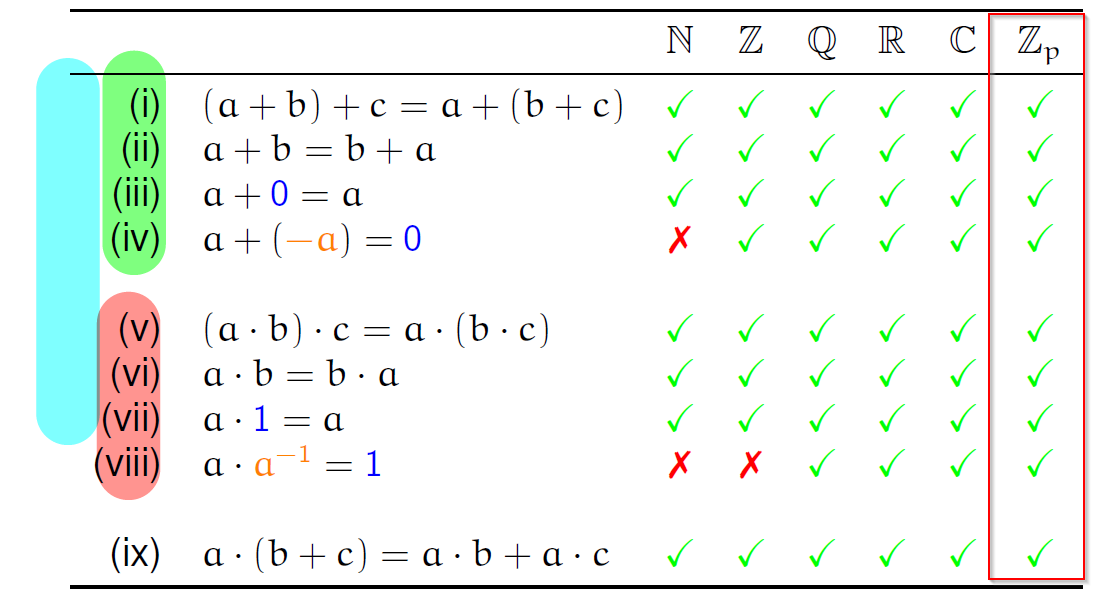
\includegraphics[scale=0.80]{img/fieldsum.png}

Wir testen das ganze mit ``p = 7''

Wichtig ist vorallem die Regel \textbf{viii}. Bei einer Primzahl p gibt
es für jedes \(a\) ein Inverses, ansonsten nicht.

    \hypertarget{the-galois-field-gf-22}{%
\subsection{\texorpdfstring{3. The Galois Field \emph{GF}
(\(2^{2}\))}{3: The Galois Field GF (2\^{}\{2\})}}\label{the-galois-field-gf-22}}

Complete the following tables for addition (top) and multiplication
(bottom).

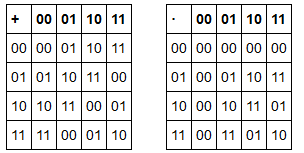
\includegraphics{img/galois_22.png}


Die allgemeinen Regeln für einen Galois Körper sind: \\
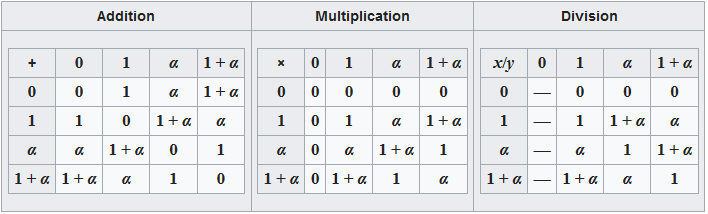
\includegraphics{img/galois_regeln.png}

\newpage

    \hypertarget{quadratic-congruence-legendre}{%
\subsection{5: Quadratic congruence
(Legendre)}\label{quadratic-congruence-legendre}}

Does the linear congruence \(x^{2} \equiv 446\) \emph{(mod 1129)} have a
solution \emph{x}?\\
You need not compute \emph{x}; just decide, if a solution exists. Use
the Legendre symbol

\((\frac{446}{1129})\)

\hypertarget{solution}{%
\subsubsection{Solution}\label{solution}}

\begin{center}
	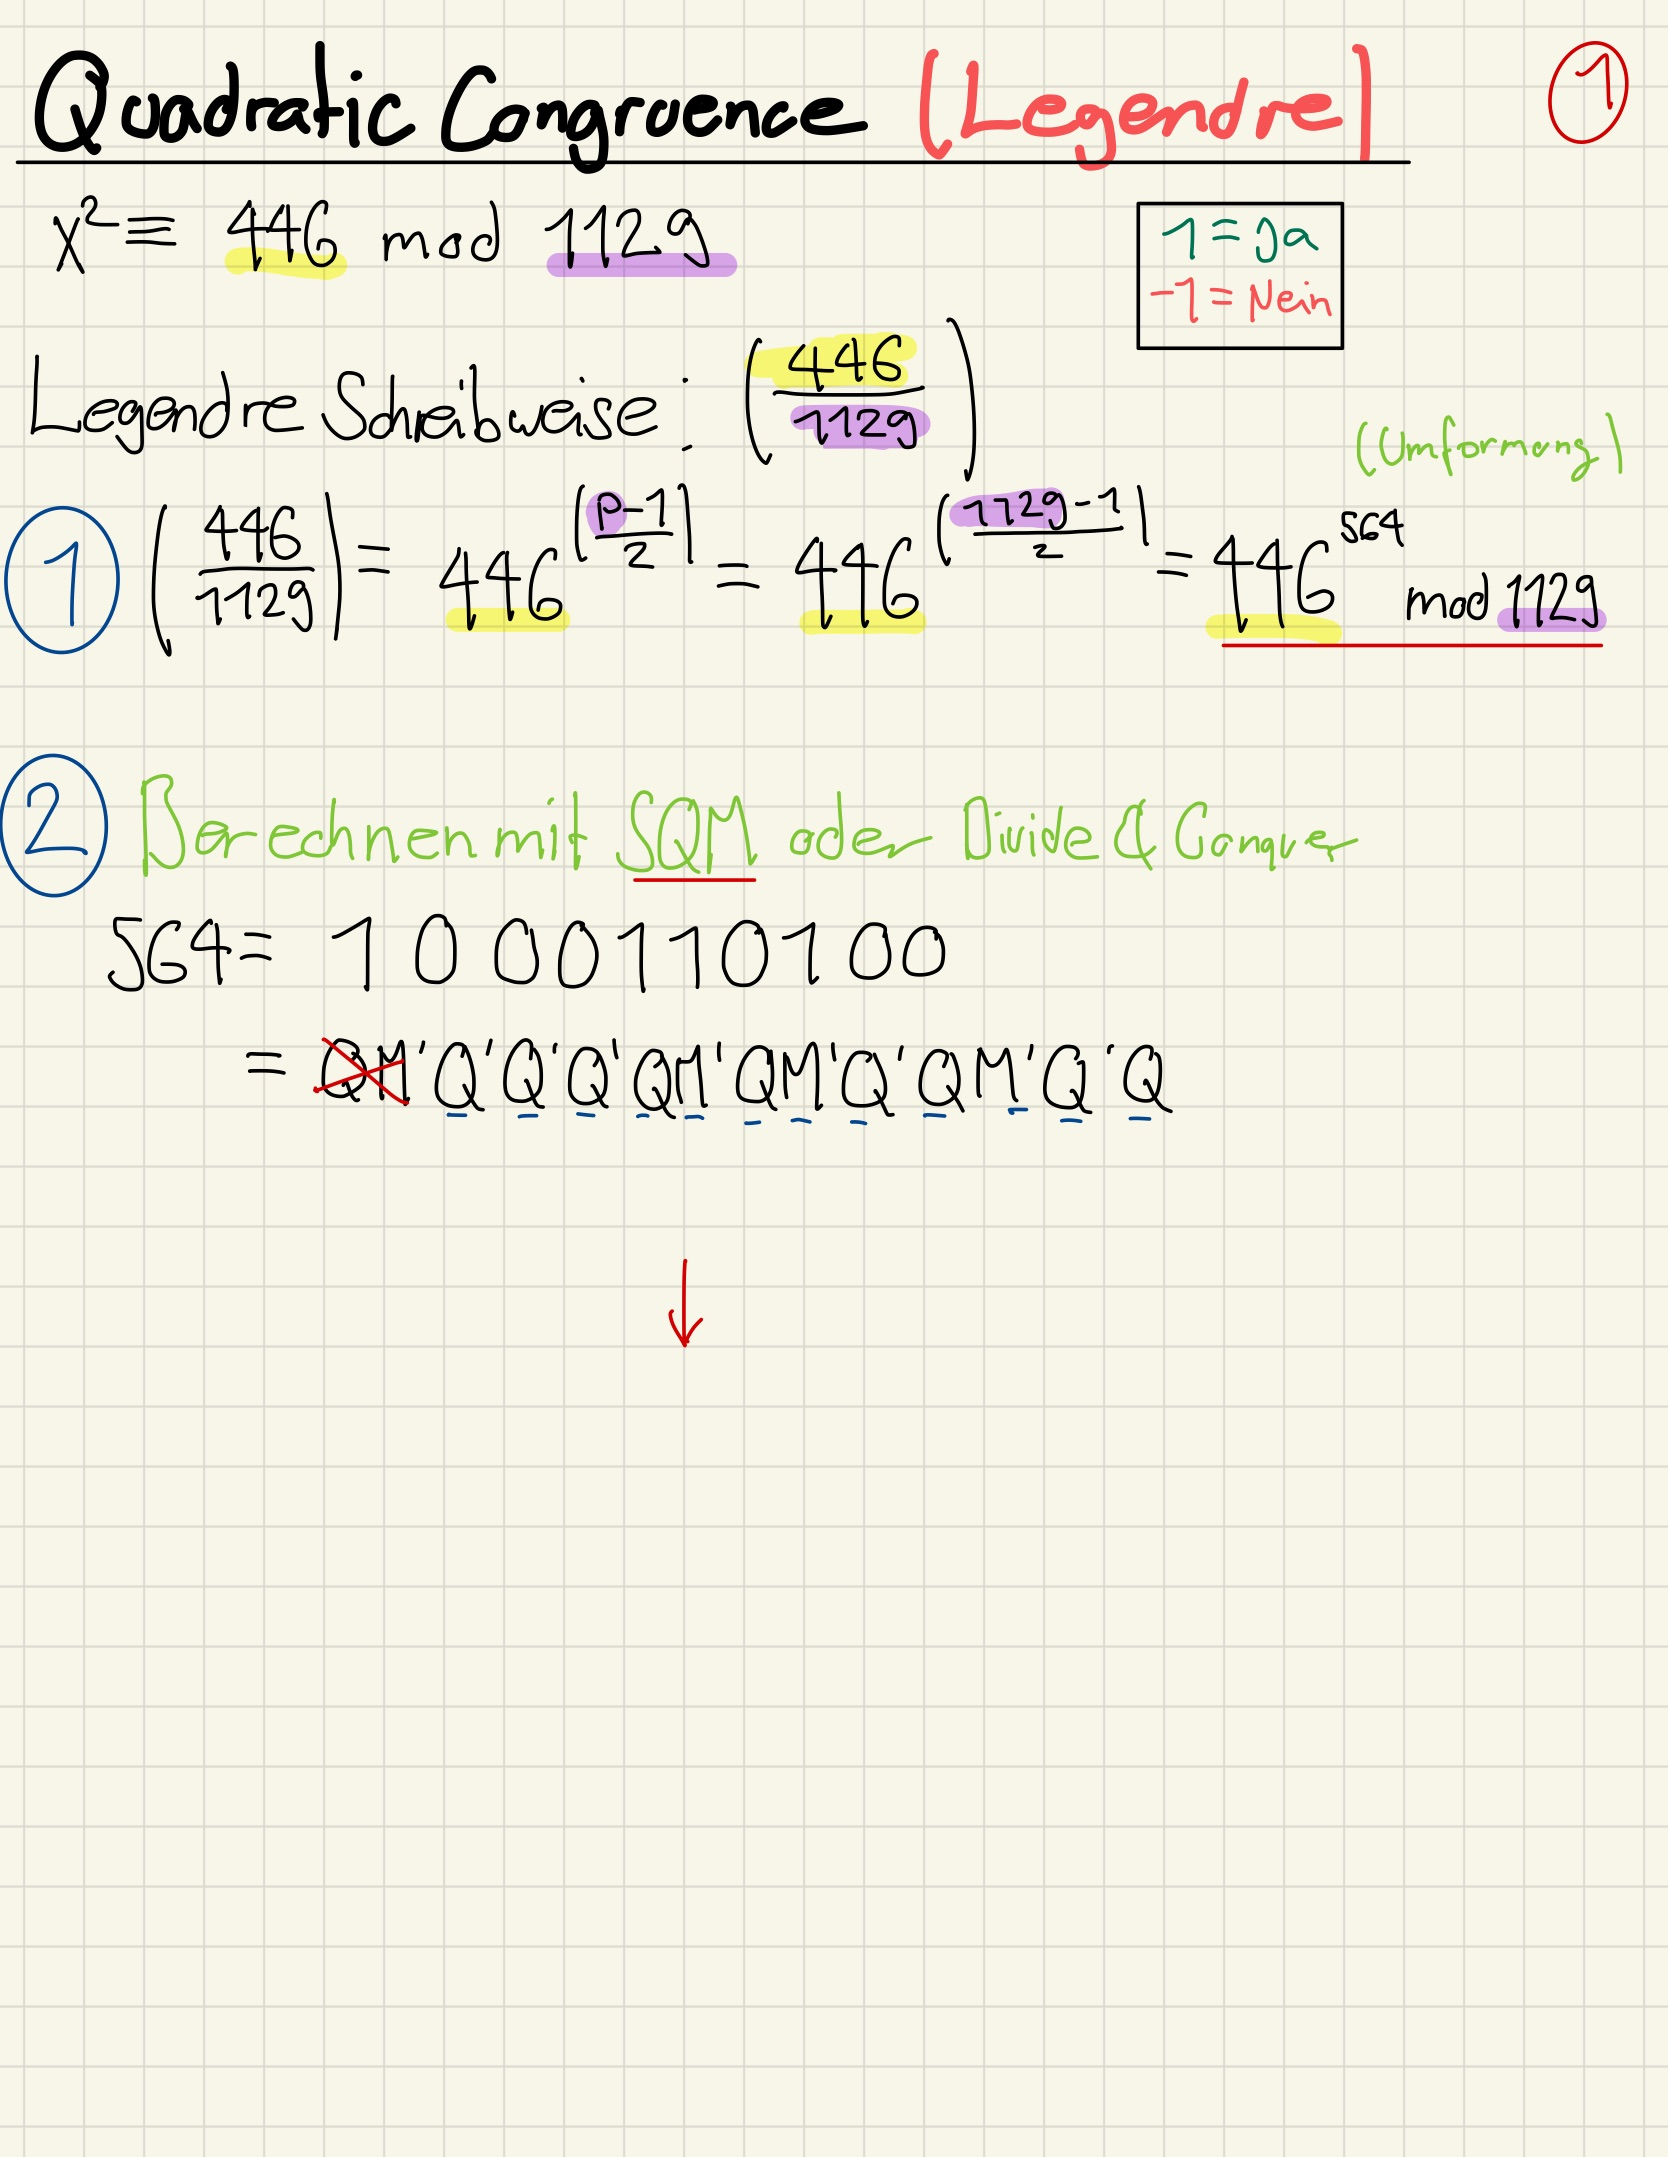
\includegraphics[scale=0.9]{img/legendre1.jpg}
	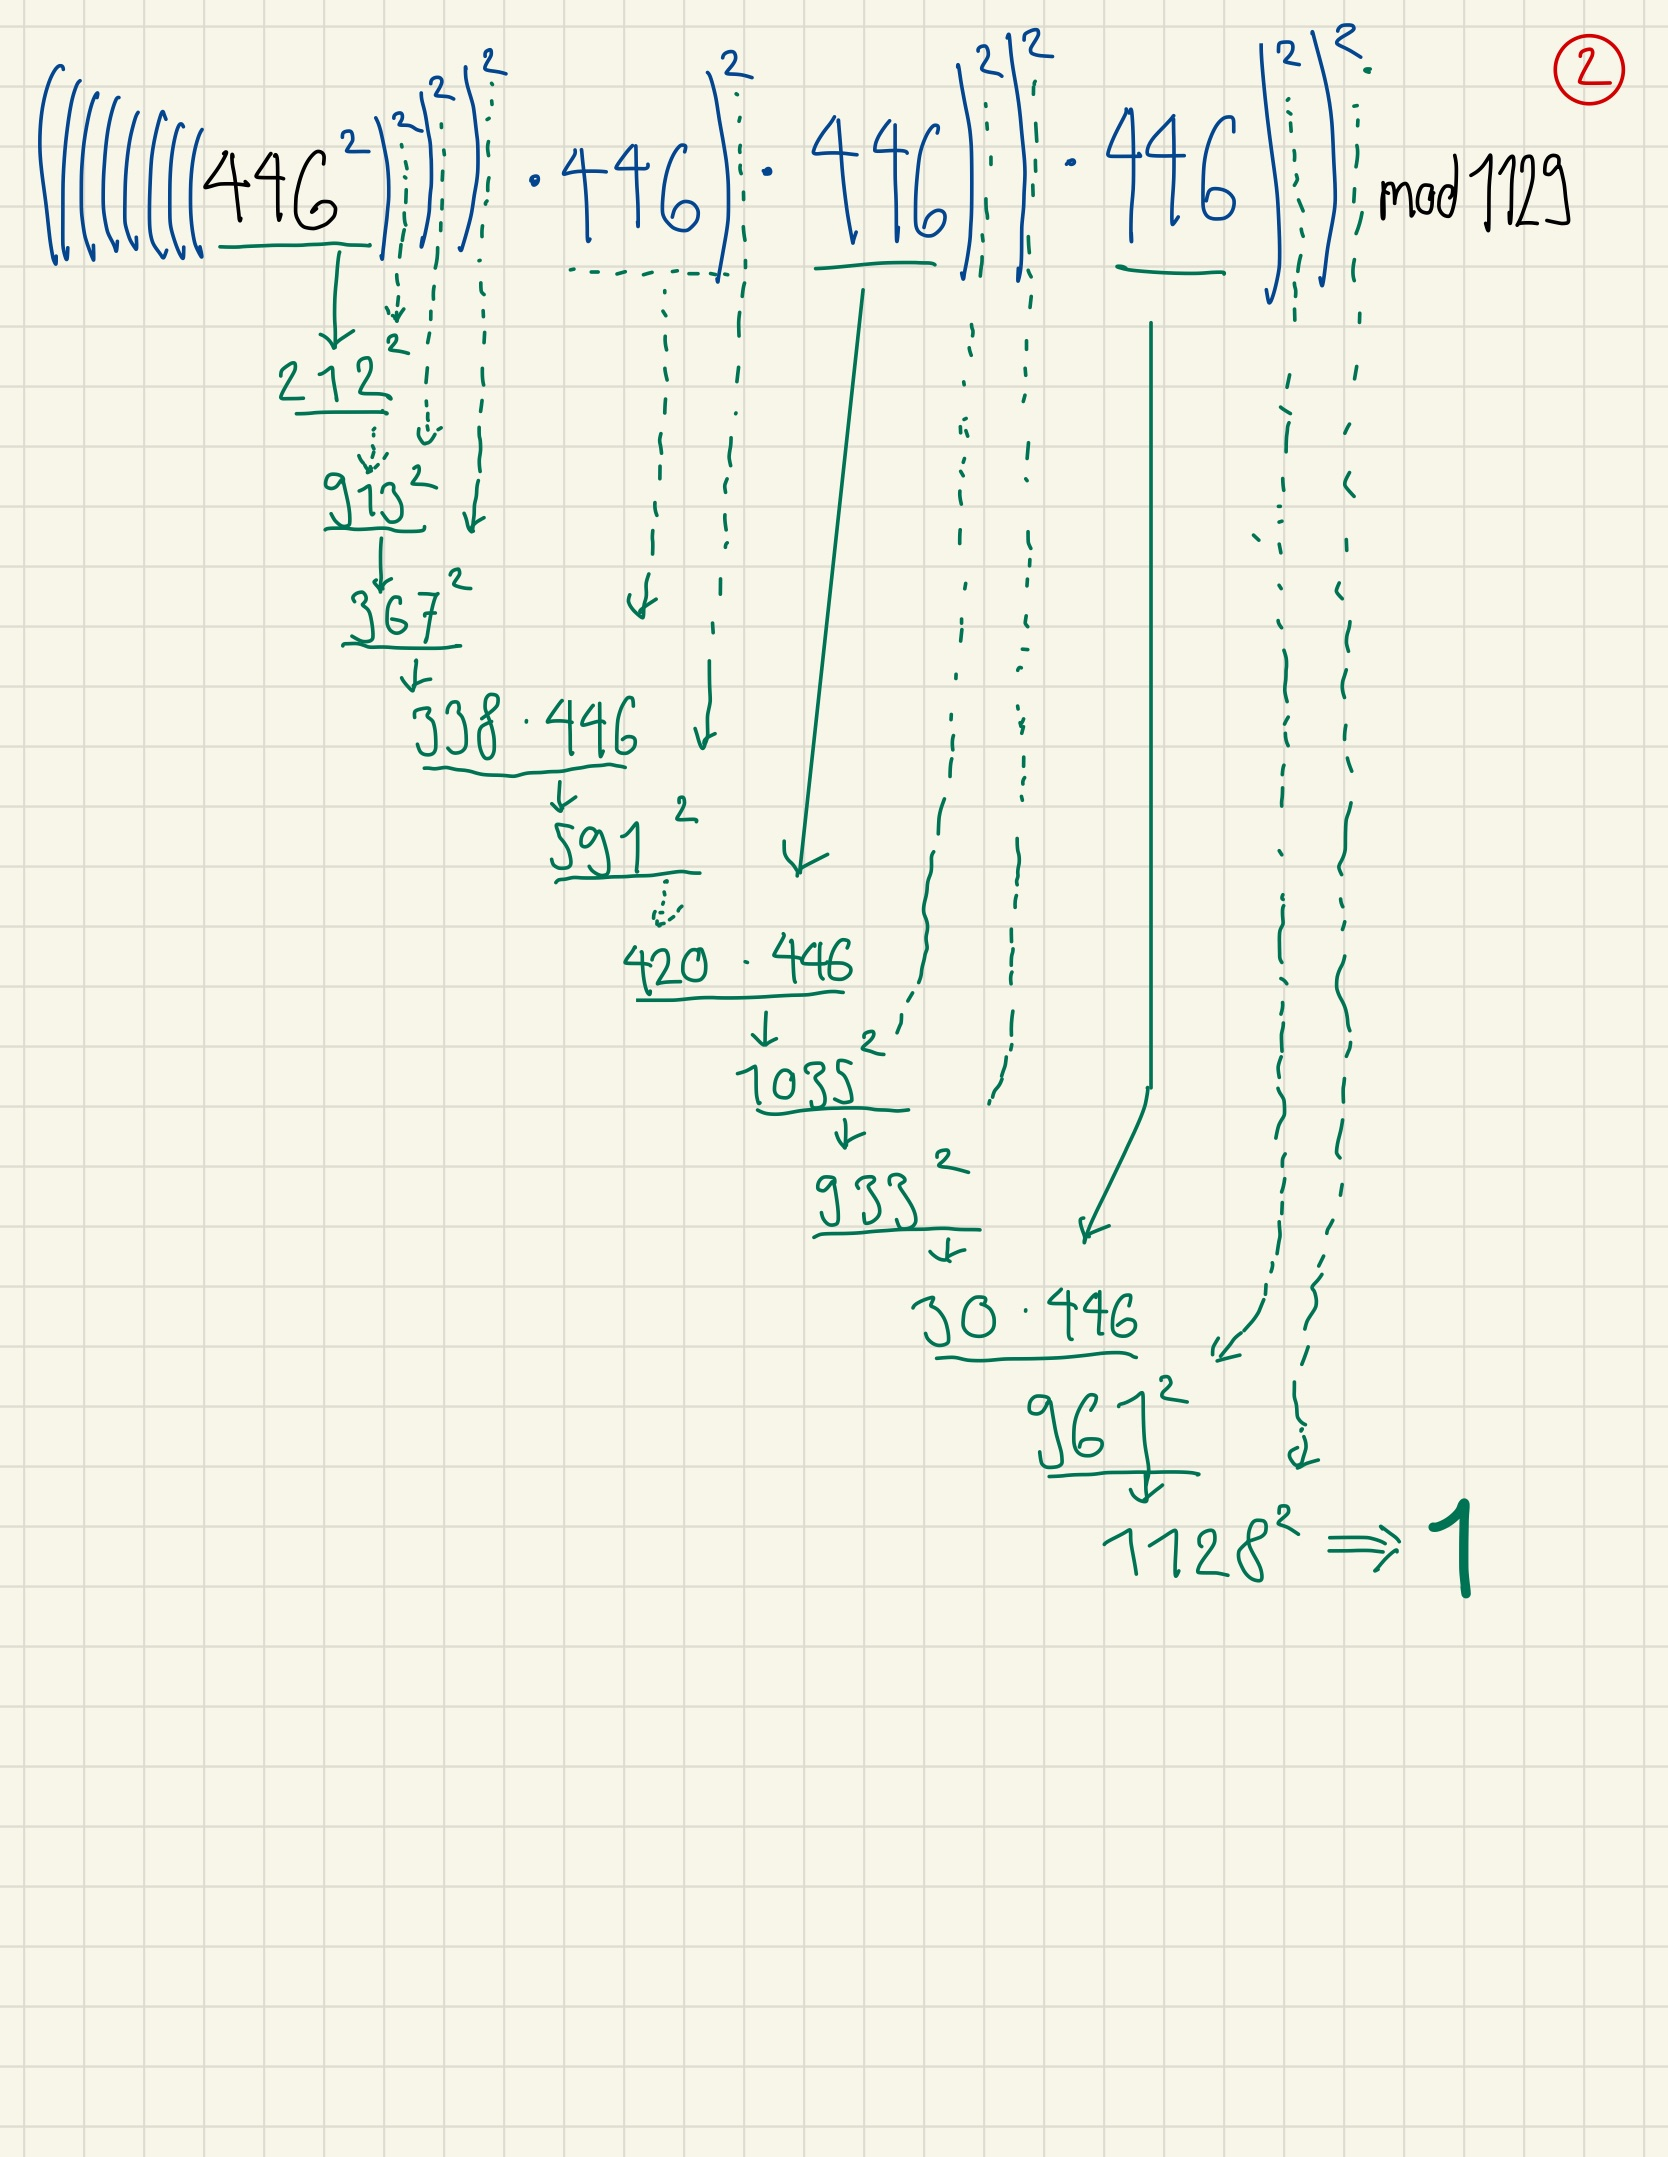
\includegraphics{img/legendre2.jpg}
\end{center}
    
\newpage 

    \hypertarget{sw03---secret-key-or-symmetric-cryptography}{%
\section{SW03 - Secret-key or symmetric
cryptography}\label{sw03---secret-key-or-symmetric-cryptography}}

    \hypertarget{des-s-box-s_3}{%
\subsection{\texorpdfstring{1. DES S-box
S\(_{3}\)}{1: DES S-box S\_\{3\}}}\label{des-s-box-s_3}}

The input to the DES S-box S3 is 110111. What's the output?

\hypertarget{solution}{%
\subsubsection{Solution}\label{solution}}


Das erste \& das letzte Bit = Reihen-Index. \textbf{11 = 3 } \\
Mittlere 4 Bits = Spalten-Index.  \textbf{1011 = 11} \\
Der Output ist somit \textbf{0011}


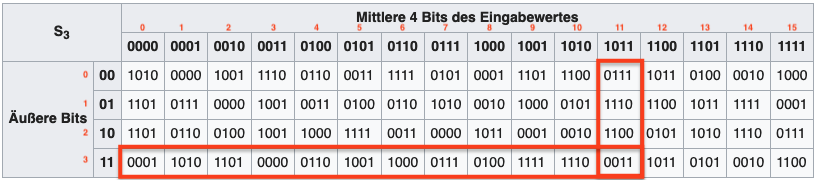
\includegraphics[scale=0.9]{img/des_sbox.png}

    \hypertarget{aes-s-box}{%
\subsection{4: AES S-box}\label{aes-s-box}}

If we input the byte 11011101 into the AES S-box, what's the output?

\hypertarget{solution}{%
\subsubsection{Solution}\label{solution}}

We split 11011101 in half, this gives us 1101 / 1101 --\textgreater{}
row / column

1101 = 13 and therefore the output is  (Hex) C1

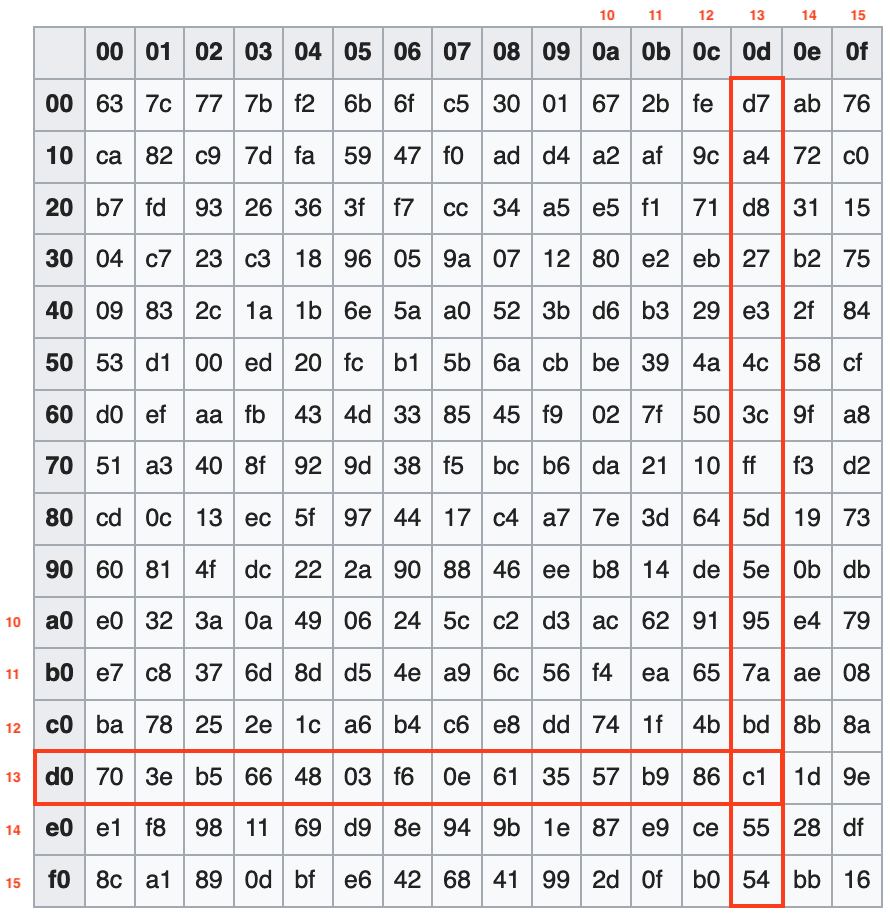
\includegraphics[scale=0.4]{img/aes_sbox.png}

Spaltenindex (erste 4 Bit): \textbf{1101}1101 == Spalte 13\\
Reihenindex (nächste 4 Bit): 1101\textbf{1101} == Reihe 13

    
\newpage

    \hypertarget{sw04---cryptographic-utilities}{%
\section{SW04 - Cryptographic
Utilities}\label{sw04---cryptographic-utilities}}

    \hypertarget{lfsr}{%
\subsection{4: LFSR}\label{lfsr}}

\textbf{Gegeben}: \\
- LFSR Länge: 5 \\
- Output: 1011001010

\hypertarget{solution}{%
\subsubsection{Solution}\label{solution}}

\begin{center}

	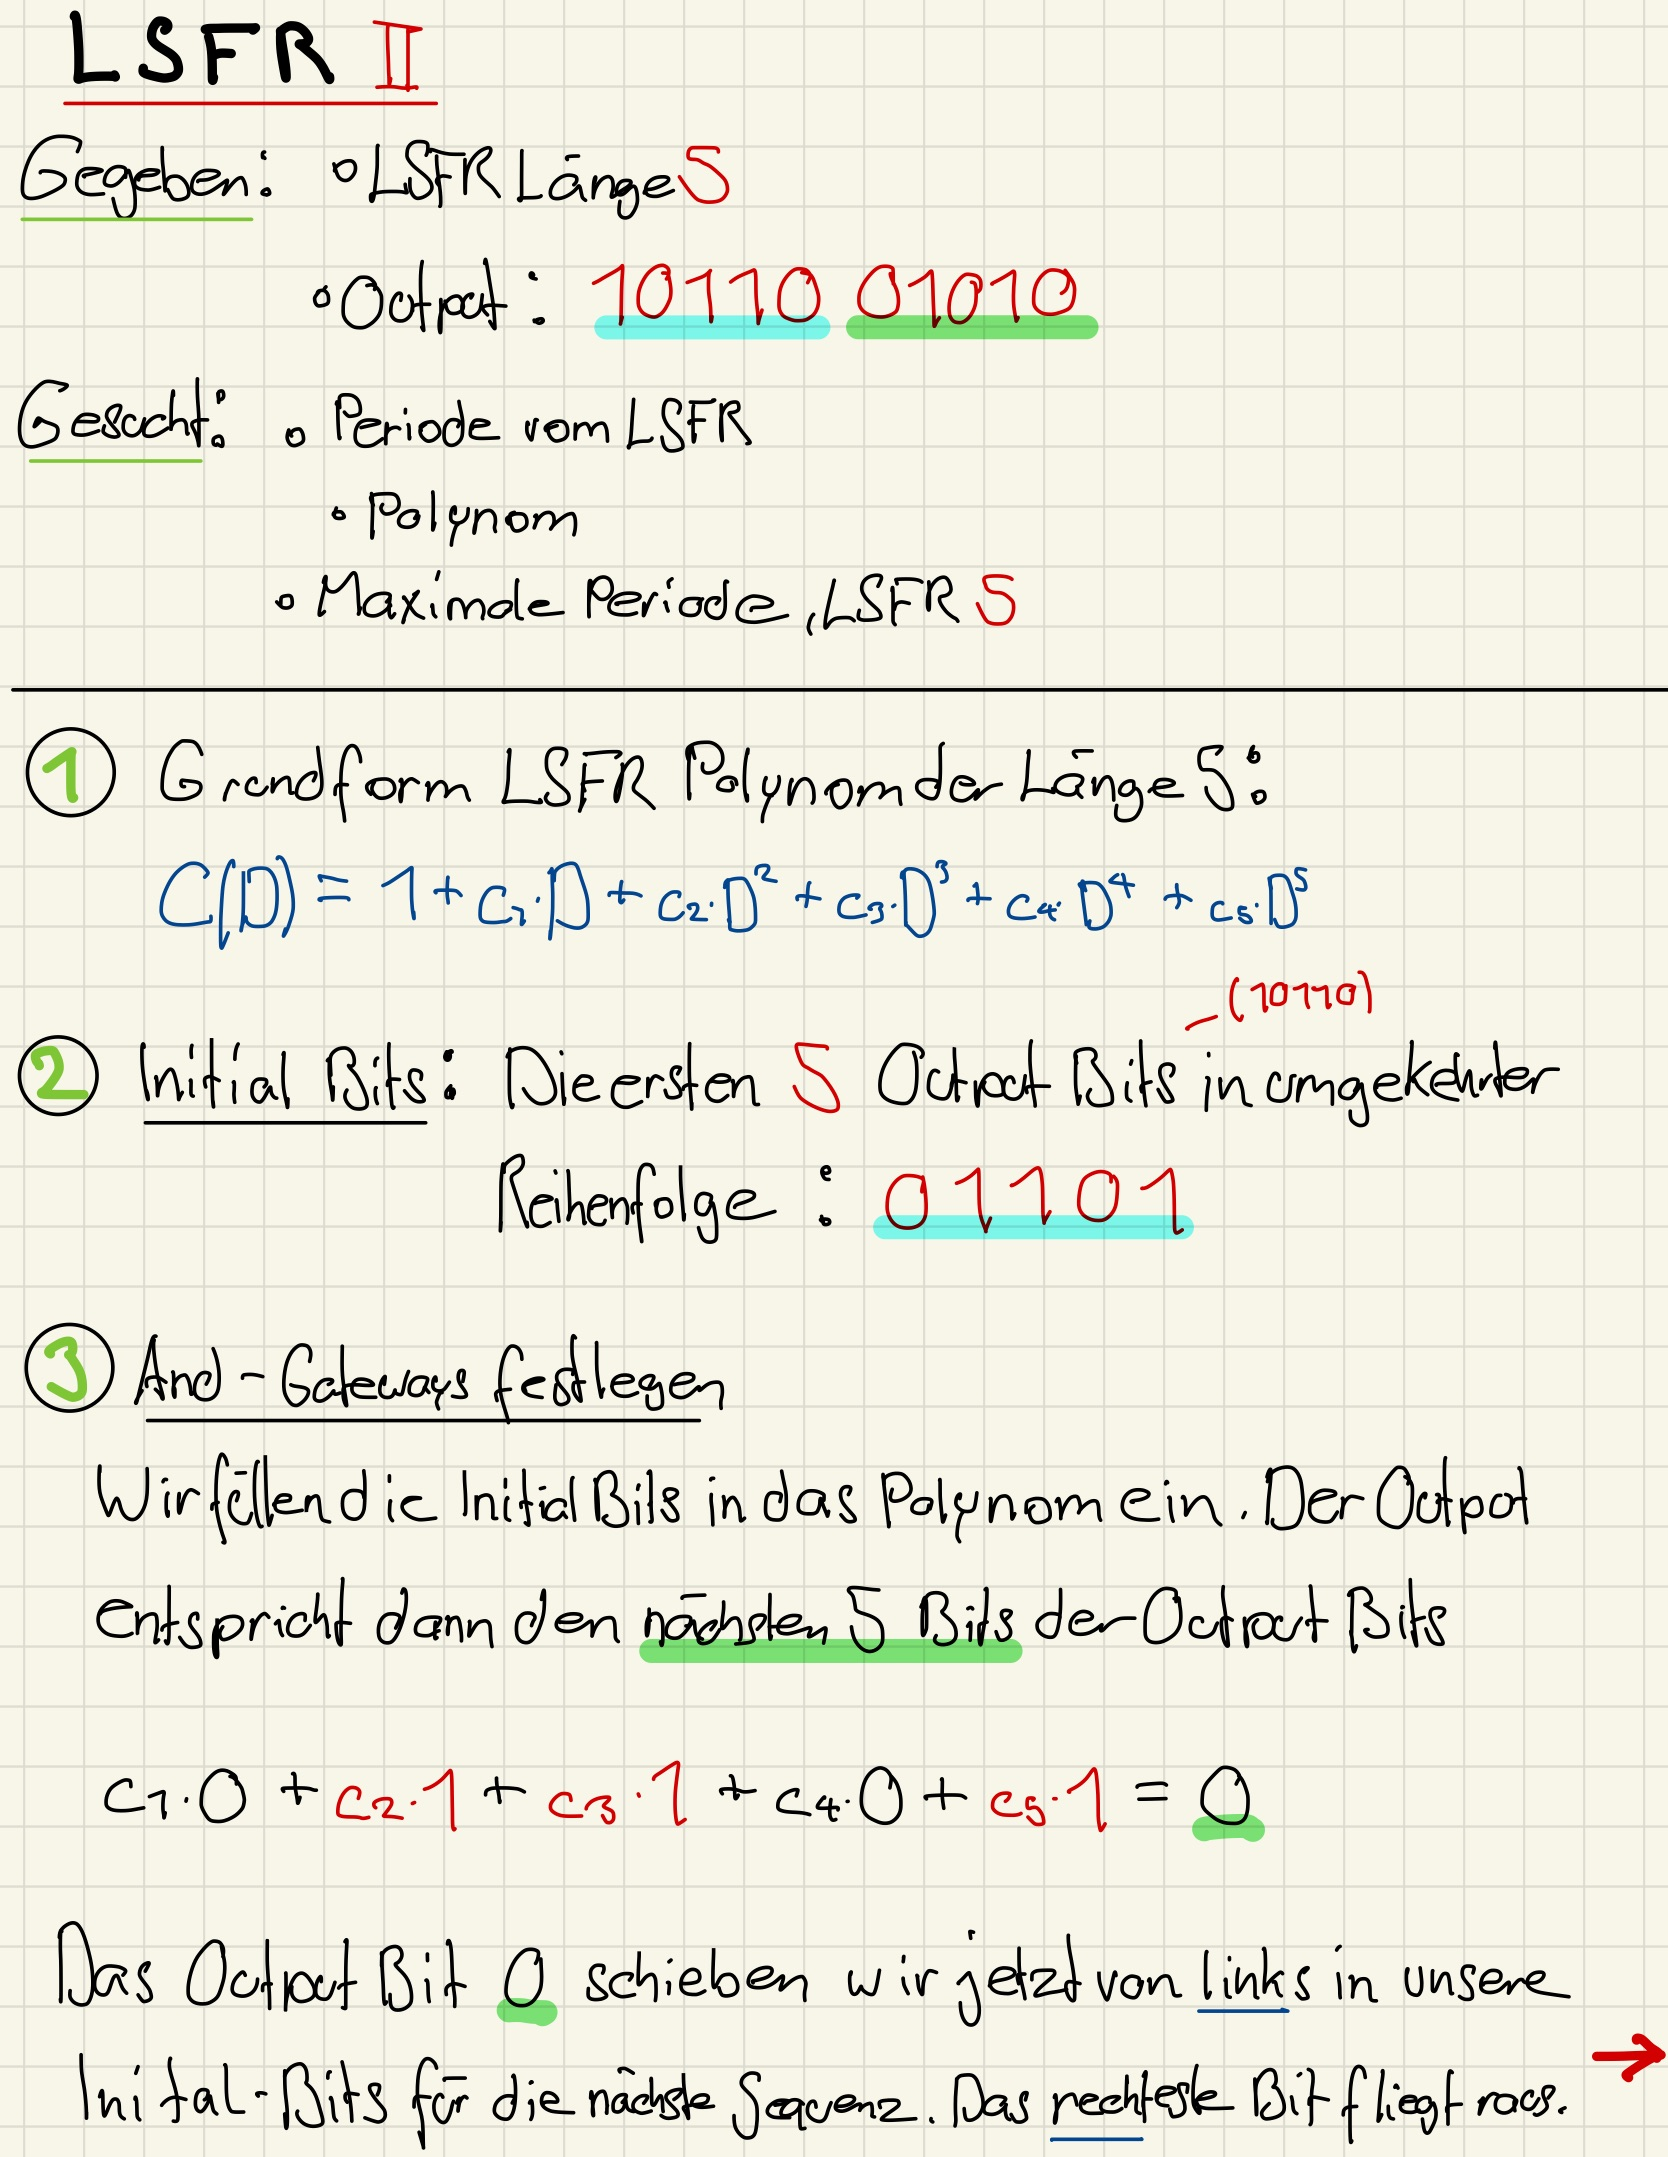
\includegraphics[scale=0.93]{img/lsfr2_1.jpg}\\
	
	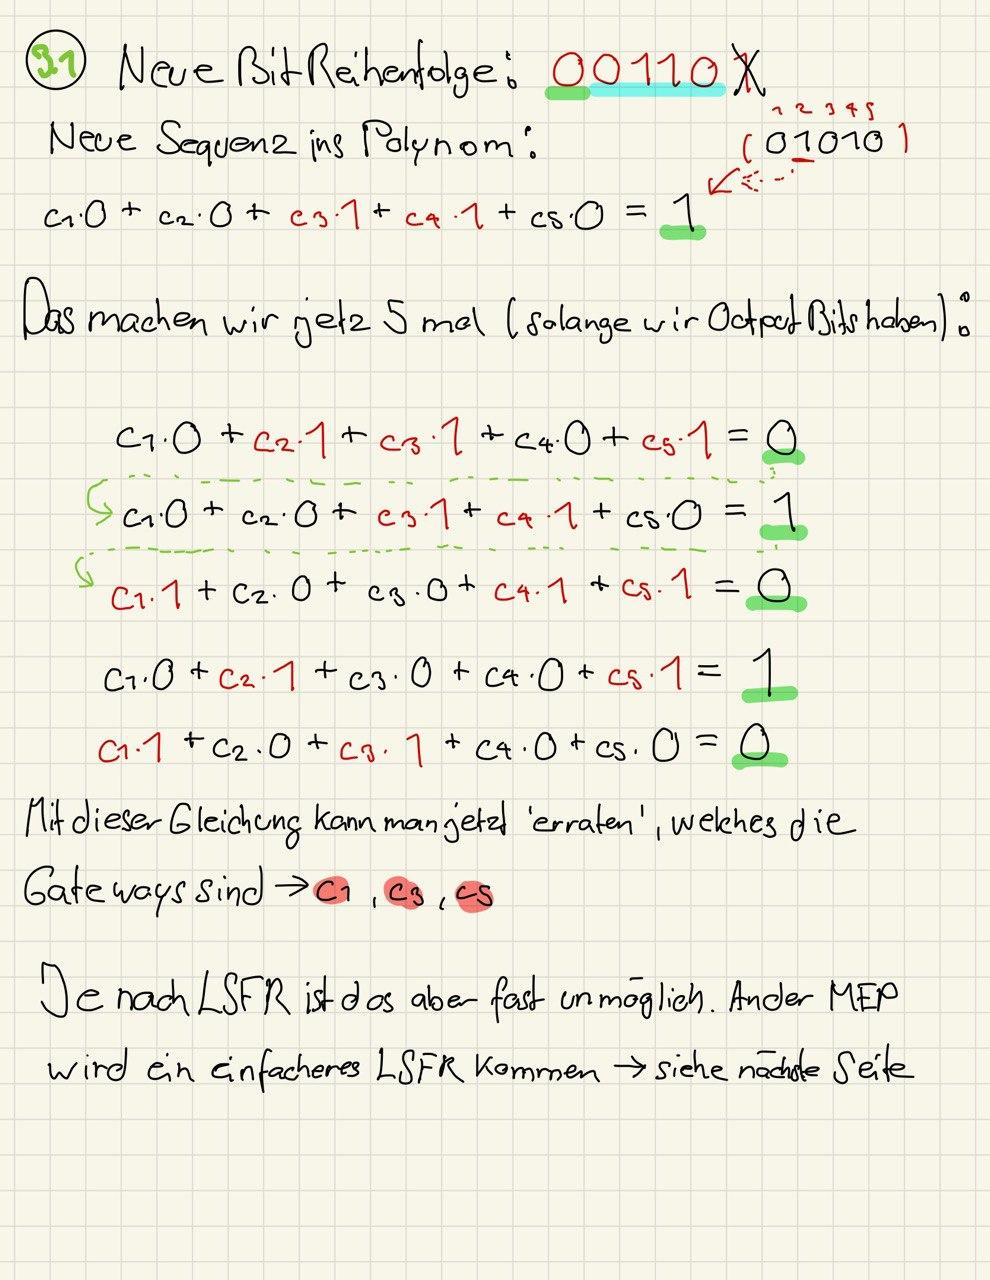
\includegraphics[scale=0.96]{img/lsfr2_2.jpg}\\
	
	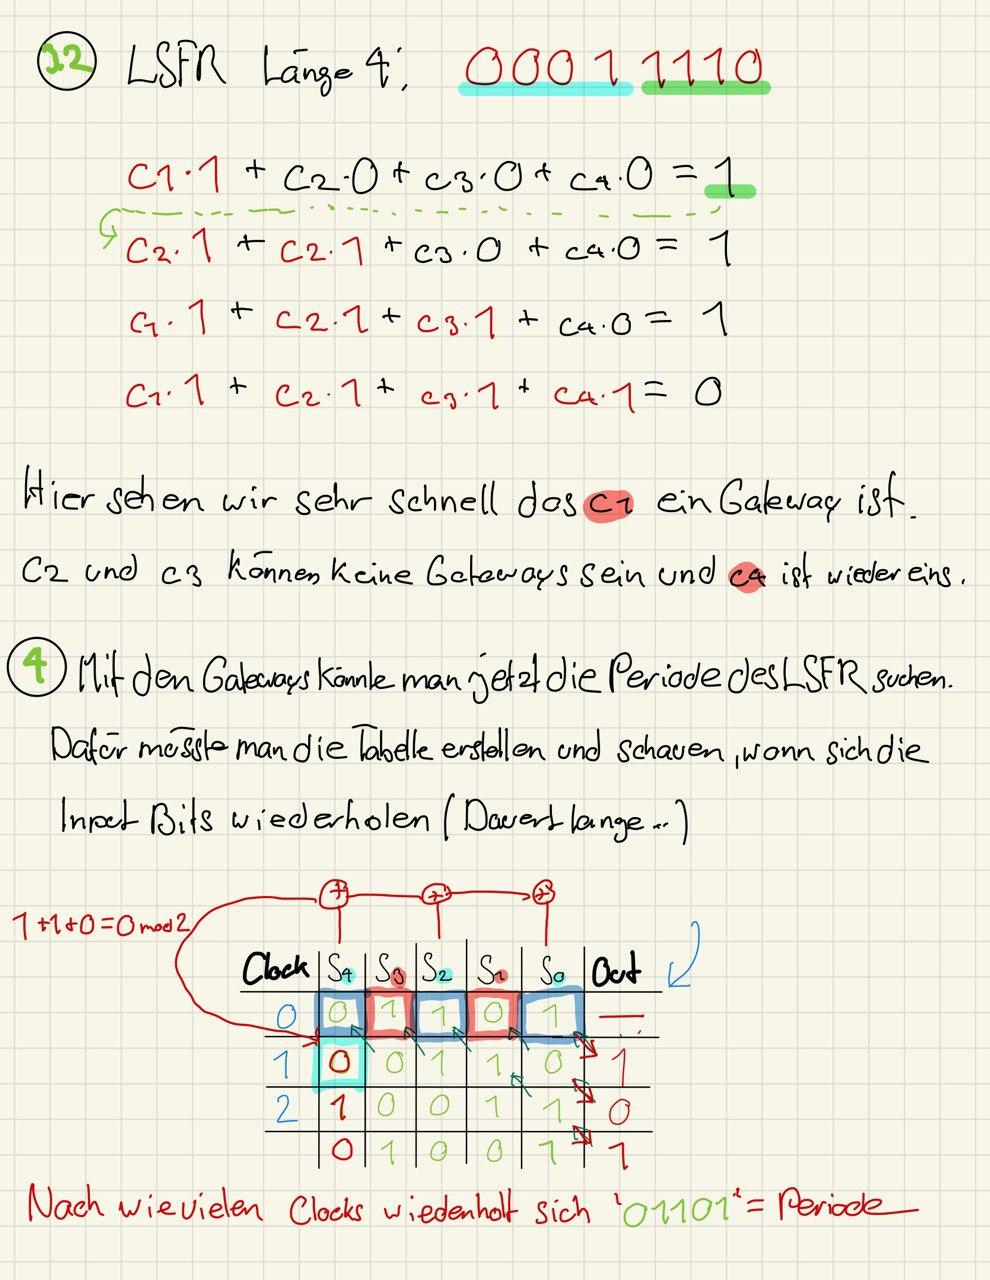
\includegraphics[scale=0.96]{img/lsfr2_3.jpg}\\
	
	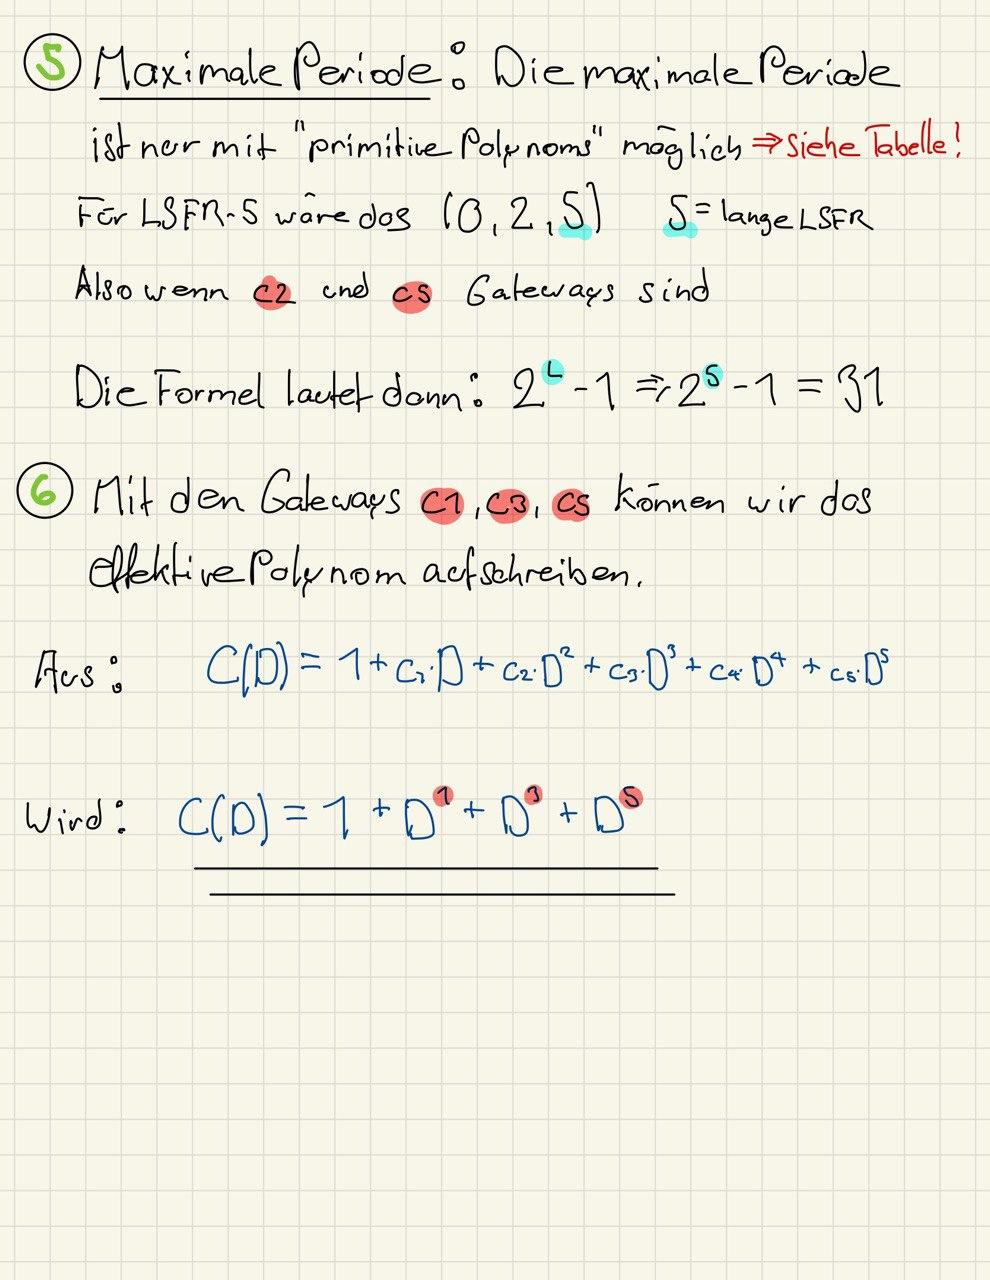
\includegraphics[scale=0.96]{img/lsfr2_4.jpg}\\

\end{center}

\hypertarget{tabelle-zum-herausfinden-des-clocks}{%
\subsubsection{Tabelle zum herausfinden des
Clocks}\label{tabelle-zum-herausfinden-des-clocks}}

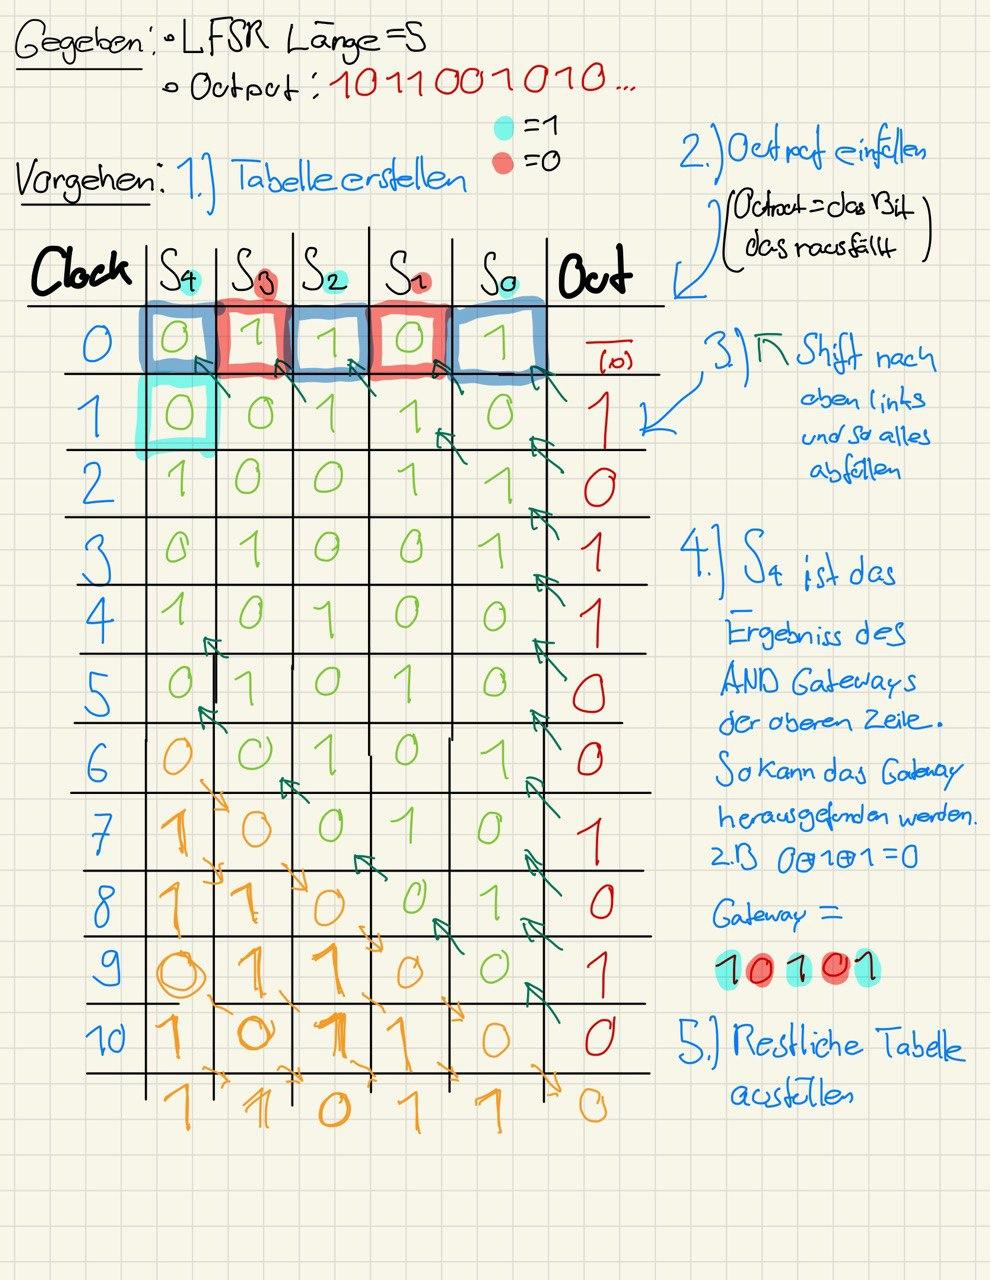
\includegraphics{img/psol2.1.jpg} \\

\subsubsection{Tabelle primitive Polynome (LSFR)}\label{tabelle-primitive-polynome-lsfr}

\begin{center}
	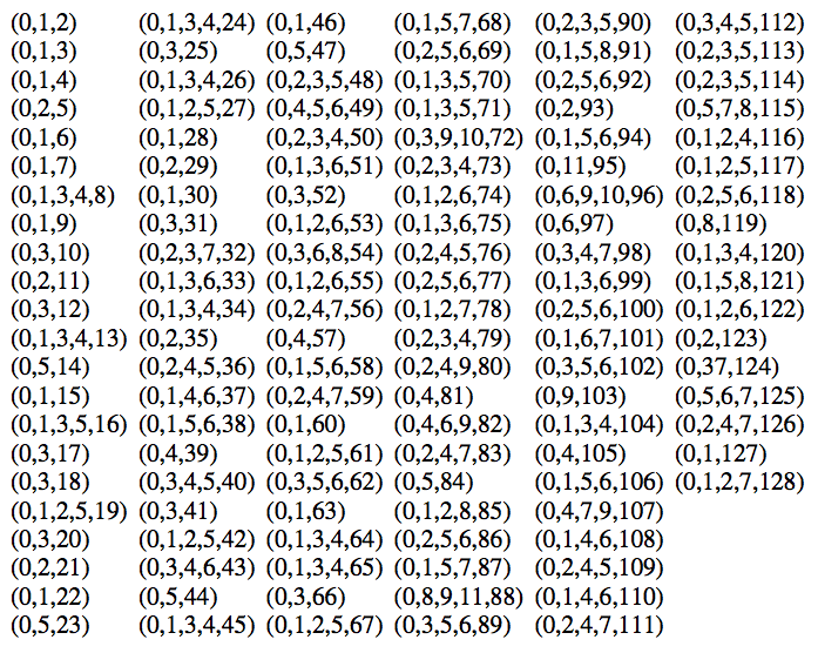
\includegraphics{img/lsfr_primitive_polynome.png}
\end{center}

Note: 0 ist immer das "Output" Register. 

\newpage

    \hypertarget{probability-for-a-collision-find-p}{%
\subsection{5: Probability for a collision (find
p)}\label{probability-for-a-collision-find-p}}

There are 40 people in a room. You bet, that there are at least 2 people
with the same birthday. What is the probability, that You win? Use the
exact formula as well as the approximation.

\hypertarget{solution}{%
\subsubsection{Solution}\label{solution}}

\textbf{Allgemein Formel für W'Keit (p) von Kollision berechnen.}

\(p = 1 - e^{\frac{-n(n-1)}{(2*m)}} = 1 - e^{\frac{-40(40-1)}{(2*365)}} = 0.882\)

n = Anzahl effektiver Werte (z.B. Personen)\\
m = Anzahl möglicher Werte (z.B. Tage im Jahr)\\
p = Wahrscheinlichkeit

    \hypertarget{probability-for-a-collision-find-n}{%
\subsection{6: Probability for a collision (find
n)}\label{probability-for-a-collision-find-n}}

Suppose You use a hash function of length 128 bits. How many hash values
would you have to compute in order to find a collision with probability
at least 90\%?

\(n = 2^{(m+1)/2} \cdot \sqrt{(\ln{(\frac{1}{1-p})}}\)

where m=128 and p=0.9.

Angenäherte Formel: \(n = 2^{\frac{m}{2}}\)

\hypertarget{solution}{%
\subsubsection{Solution}\label{solution}}

\(n = 2^{(m+1)/2} \cdot \sqrt{(\ln{(\frac{1}{1-p})}} = 2^{(128+1)/2} \cdot \sqrt{(\ln{(\frac{1}{1-0.9})}} = 3.958 \cdot 10^{19}\)

    

    \hypertarget{sw05---public-key-cryptography-i}{%
\section{SW05 - Public Key Cryptography
I}\label{sw05---public-key-cryptography-i}}

    \hypertarget{shamirs-three-pass-protocol}{%
\subsection{1: Shamir's three-pass
protocol}\label{shamirs-three-pass-protocol}}

Alice and Bob want the implement Shamir's three-pass protocol using the
Vernam cipher, i.e.~one-time pad. This is supposed to provide perfect
secrecy. Is the following protocol secure?

\begin{center}
	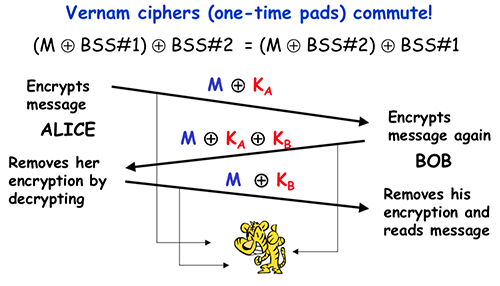
\includegraphics{img/VernamCiphers.png}
\end{center}


\textbf{Your Task}: Can You compute the message? Make an example with
\(M = 010110111101\), \(K_A = 101101110100\), and
\(K_B = 001011011011\).

\hypertarget{solution}{%
\subsubsection{Solution}\label{solution}}

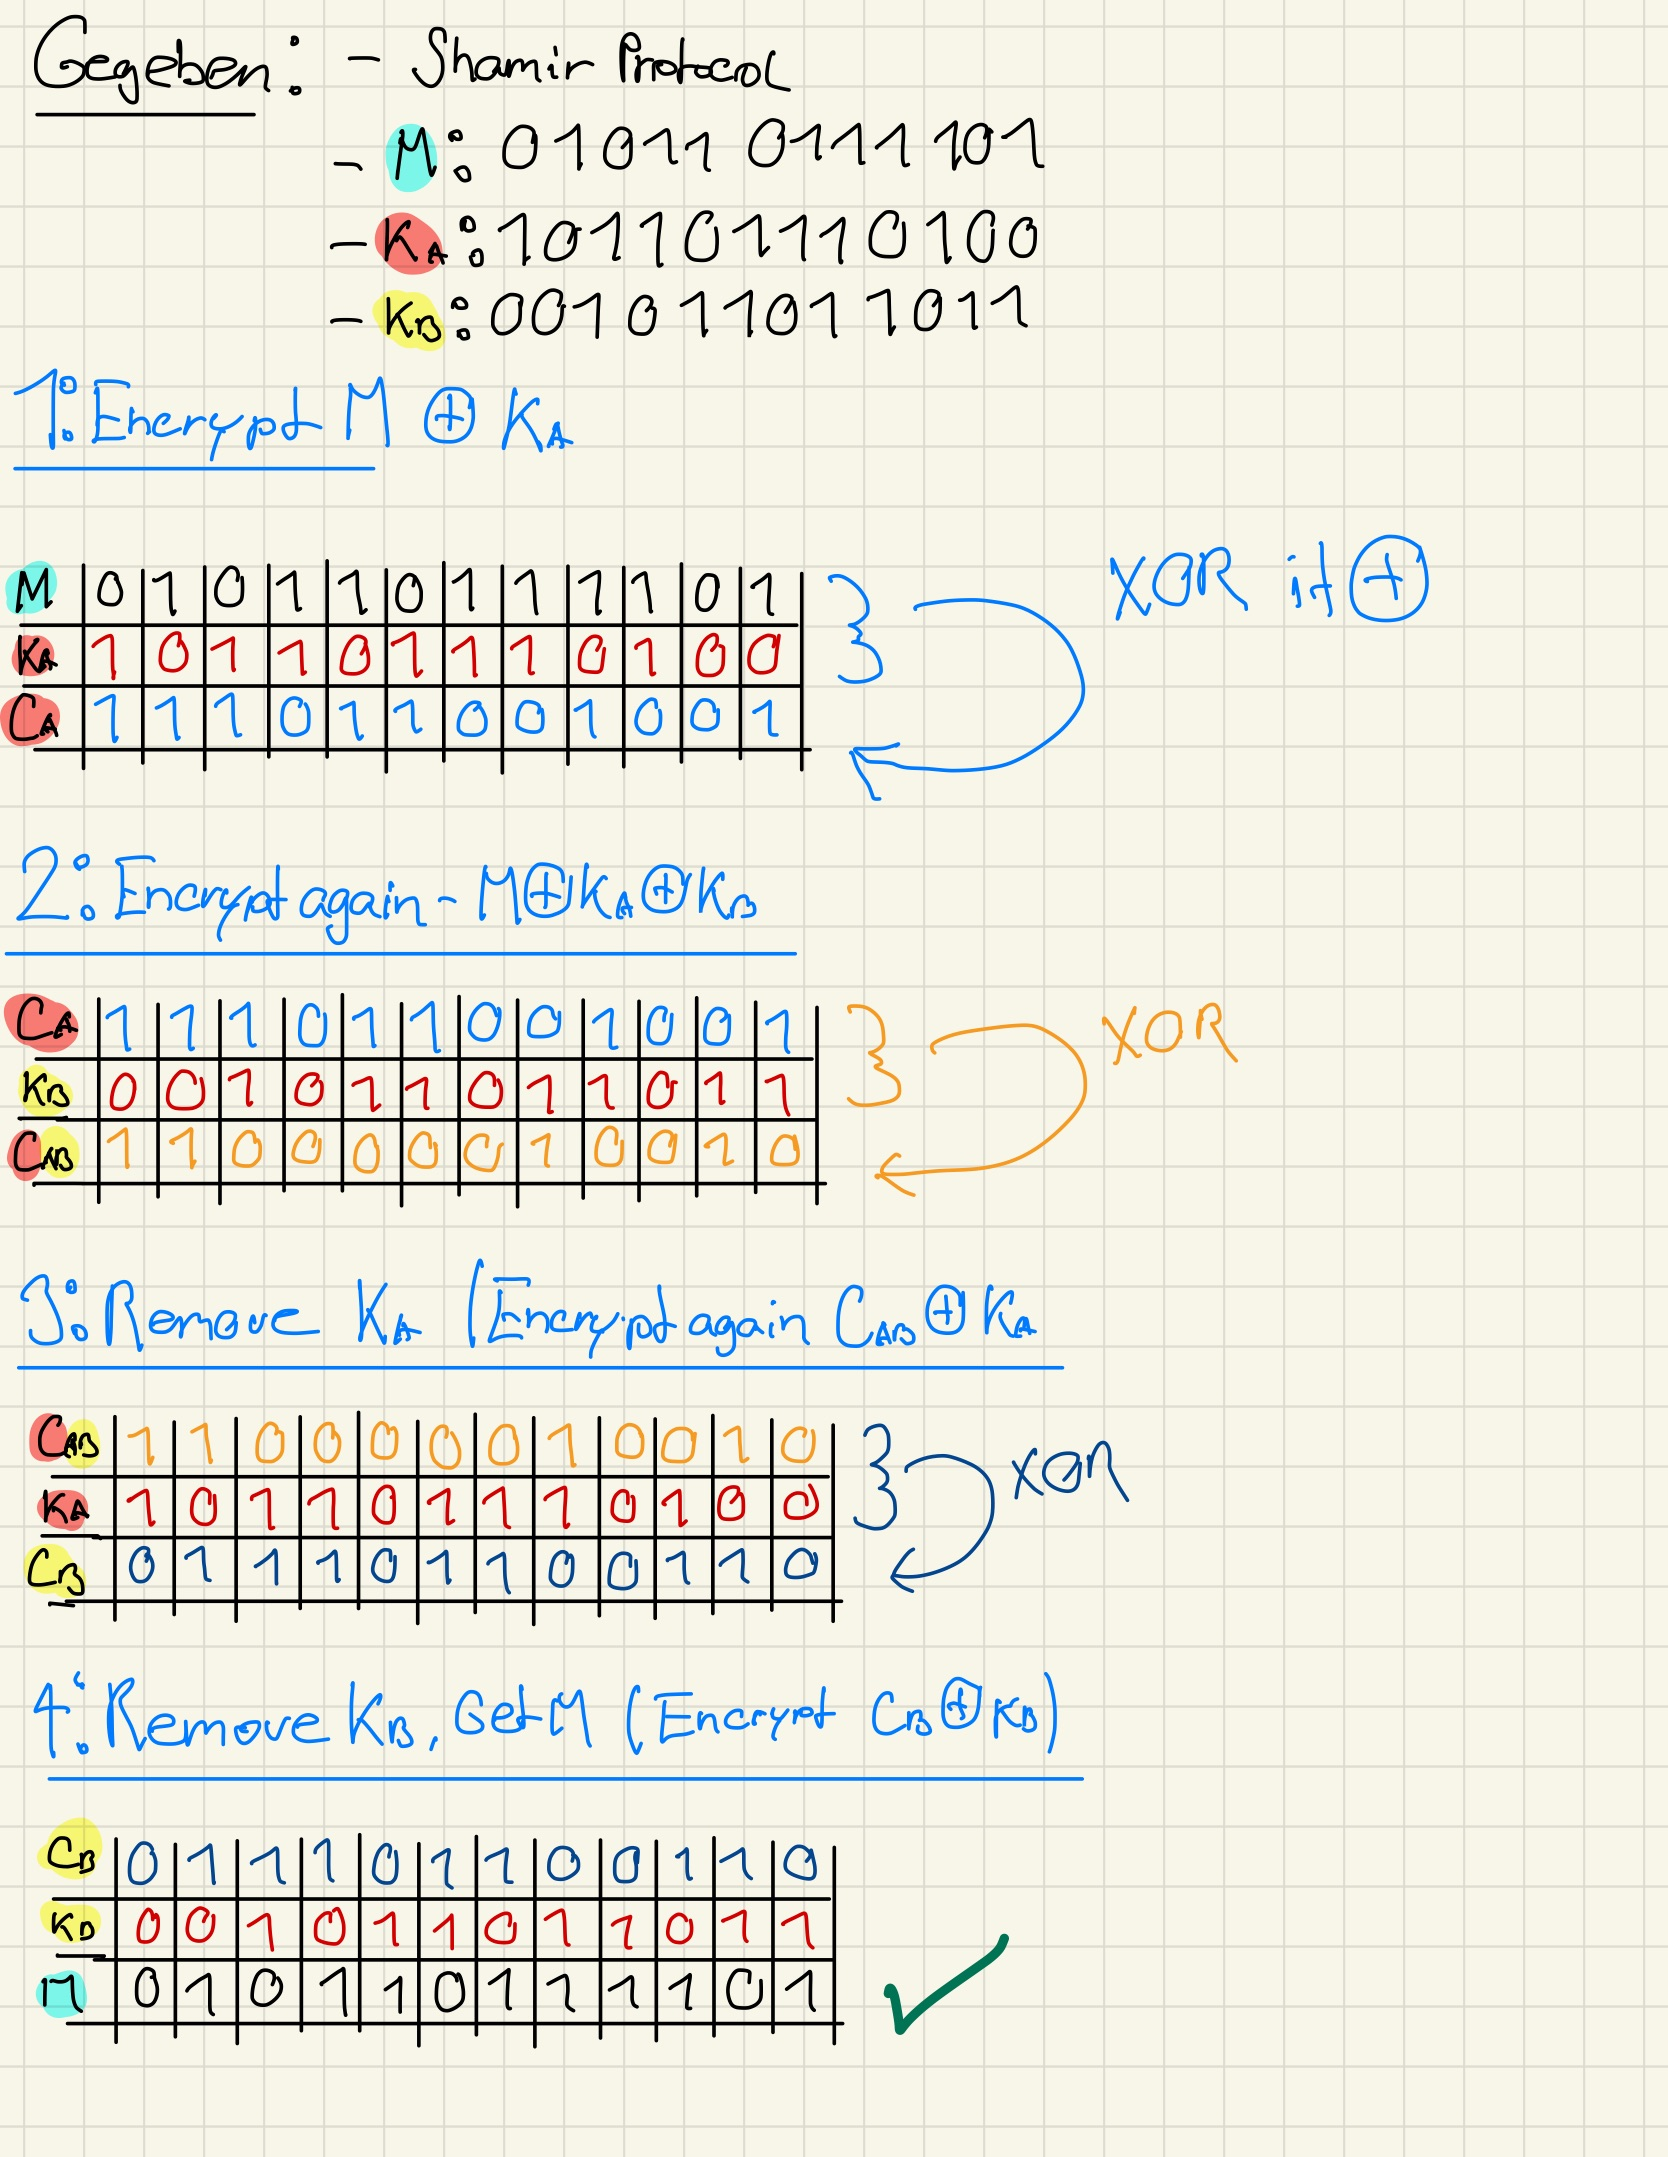
\includegraphics{img/psol3.jpg}

\newpage

    \hypertarget{diffie-hellman}{%
\subsection{2: Diffie Hellman}\label{diffie-hellman}}

\emph{Alice} and \emph{Bob} agree to use \(n = 13\) and \(e = 11\).
Alice chooses her secret number \(a = 5\), whereas Bob chooses
\(b = 7\).

\textbf{Your Task}: What are the requirements for \(n\) and \(e\)? Are
they fullfilled? Describe the key agreement protocol step by step using
the above assumptions about a and b. What is the common secret key?

\hypertarget{solution}{%
\subsubsection{Solution}\label{solution}}

\(e\) must be a generator for \(\mathbb{Z}_n^*\), this is true for
\(e = 11\) to \(n=13\)


\begin{center}
	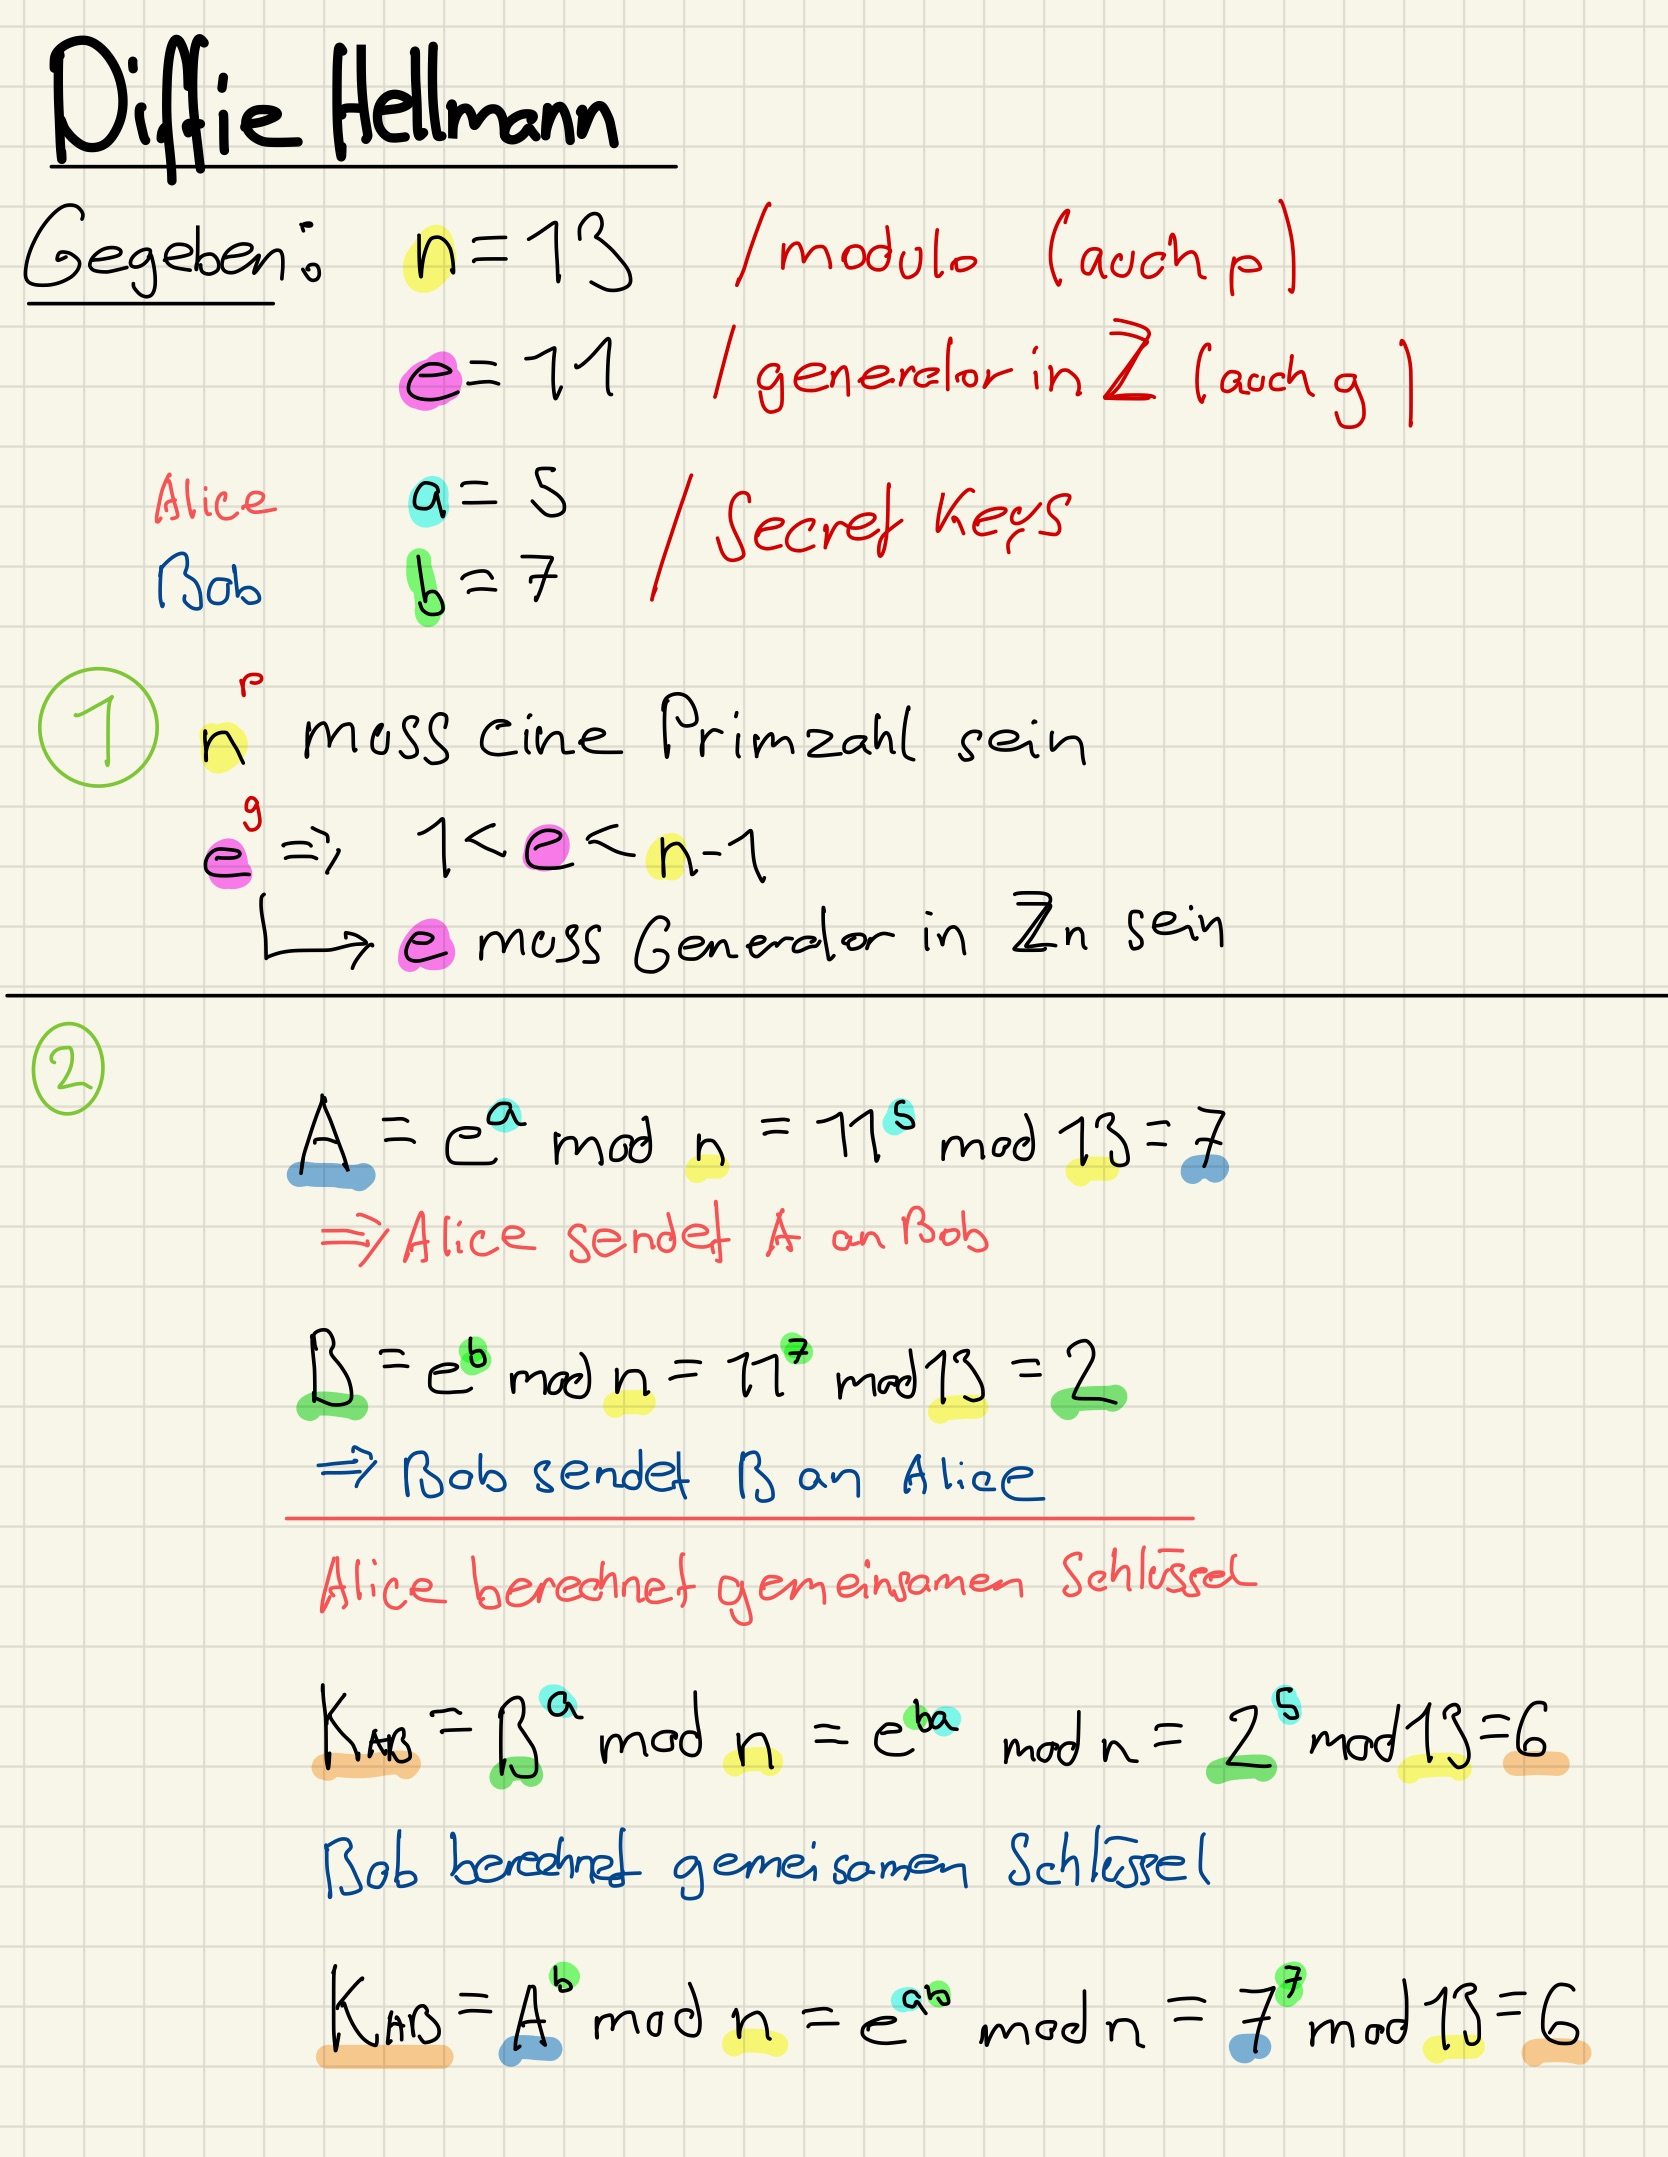
\includegraphics[scale=0.85]{img/diffieh.jpg}
\end{center}


    \hypertarget{discrete-logarithm-problem}{%
\subsection{3: Discrete Logarithm
Problem}\label{discrete-logarithm-problem}}

Assume Mallory intercepts the message \(A = 9\) from Alice to Bob and
\(B = 3\) from Bob to Alice. He also knows \(n = 13\) and \(g = 11\).

\textbf{Your Task}: Suppose Mallory wants to know the common key.
Describe his steps to find this key!

\hypertarget{solution}{%
\subsubsection{Solution}\label{solution}}

He would need to find \(a\) such that \(A=g^a \mod n\). Then he could
calculate \(B^a=K \rightarrow(g^{b \cdot a})\).

\(9=11^a \mod 13\)

\(11^1 = 11\)

\(...\)

\(11^8 = 9 -> a=8 \rightarrow K = B^a = 3^8 \bmod 13 = 9\)

For large numbers, this is \textbf{infeasable}.

    \hypertarget{rsa-ablauf}{%
\subsection{4.0 - RSA Ablauf}\label{rsa-ablauf}}

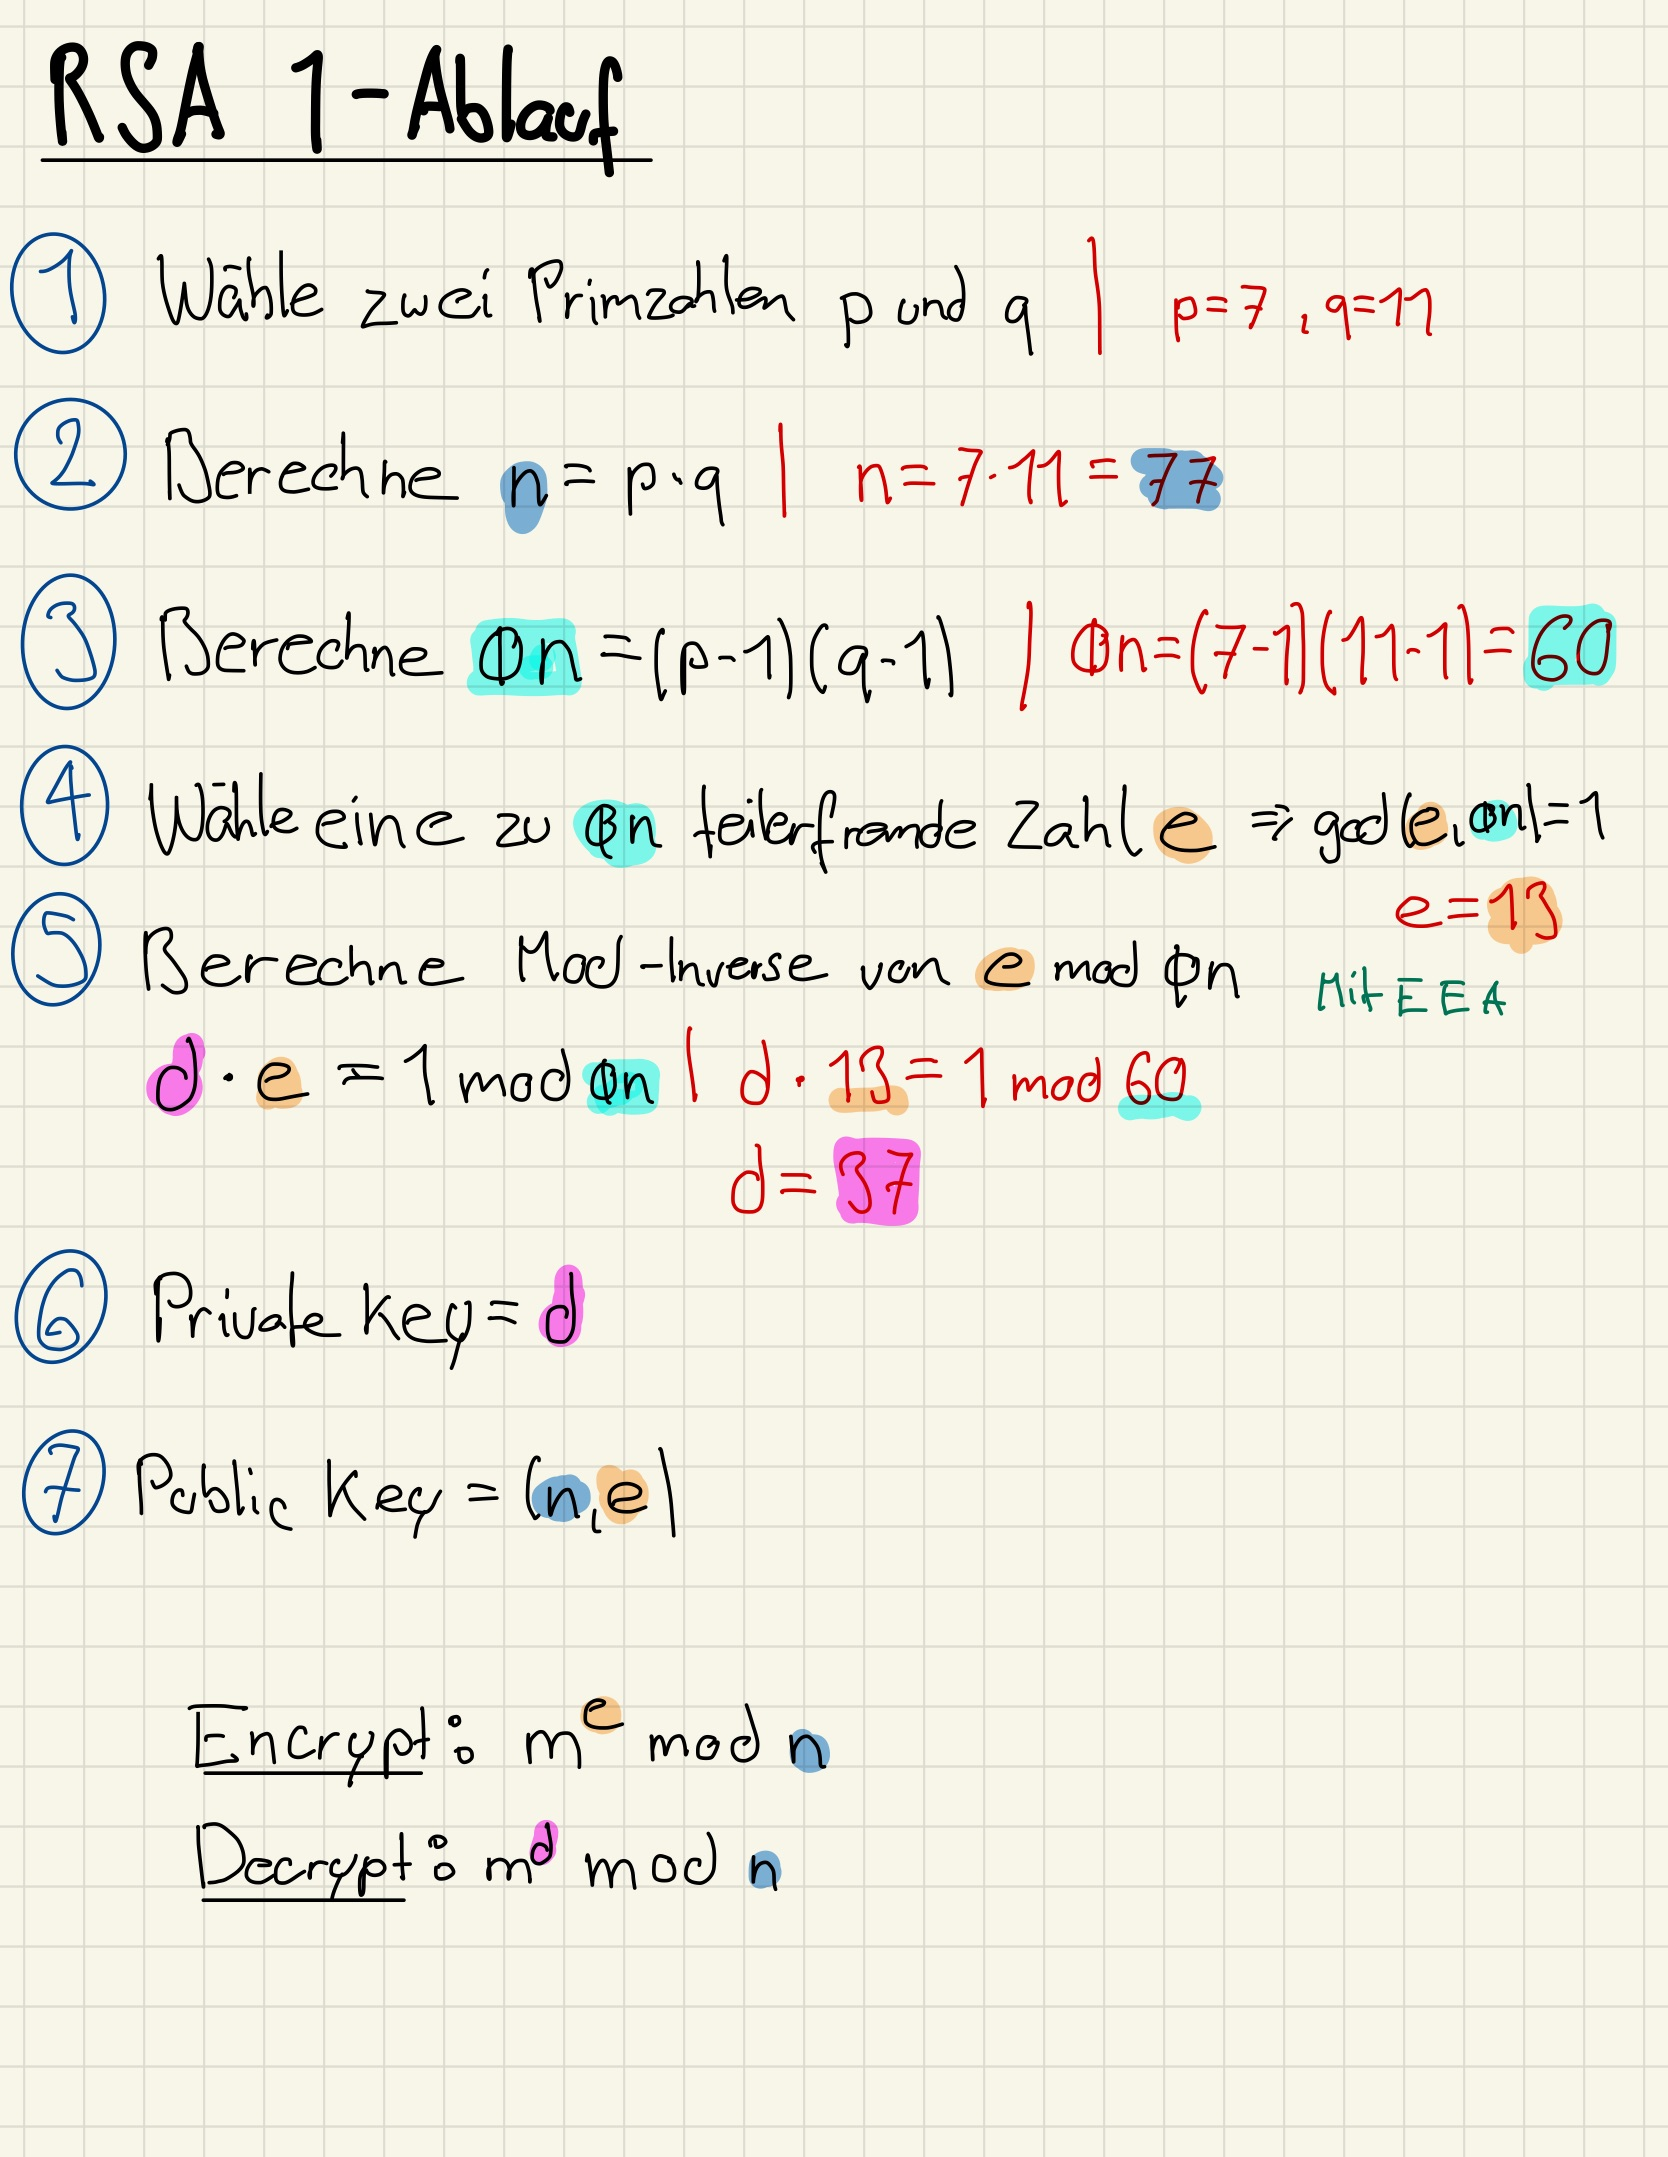
\includegraphics{img/rsa_ablauf.jpg}

\newpage

    \hypertarget{attack-on-textbook-rsa-factorizing-n}{%
\subsection{4.1 - Attack on textbook RSA (factorizing
n)}\label{attack-on-textbook-rsa-factorizing-n}}

The public key \((n,e) = (2537,13)\) was used to encrypt the plaintext
\(M\). Eve intercepts the ciphertext \(C = 2081\).

\textbf{Your Task}: Show how Eve computes the plaintext \(M\)!

\hypertarget{solution}{%
\subsubsection{Solution}\label{solution}}

\begin{center}
	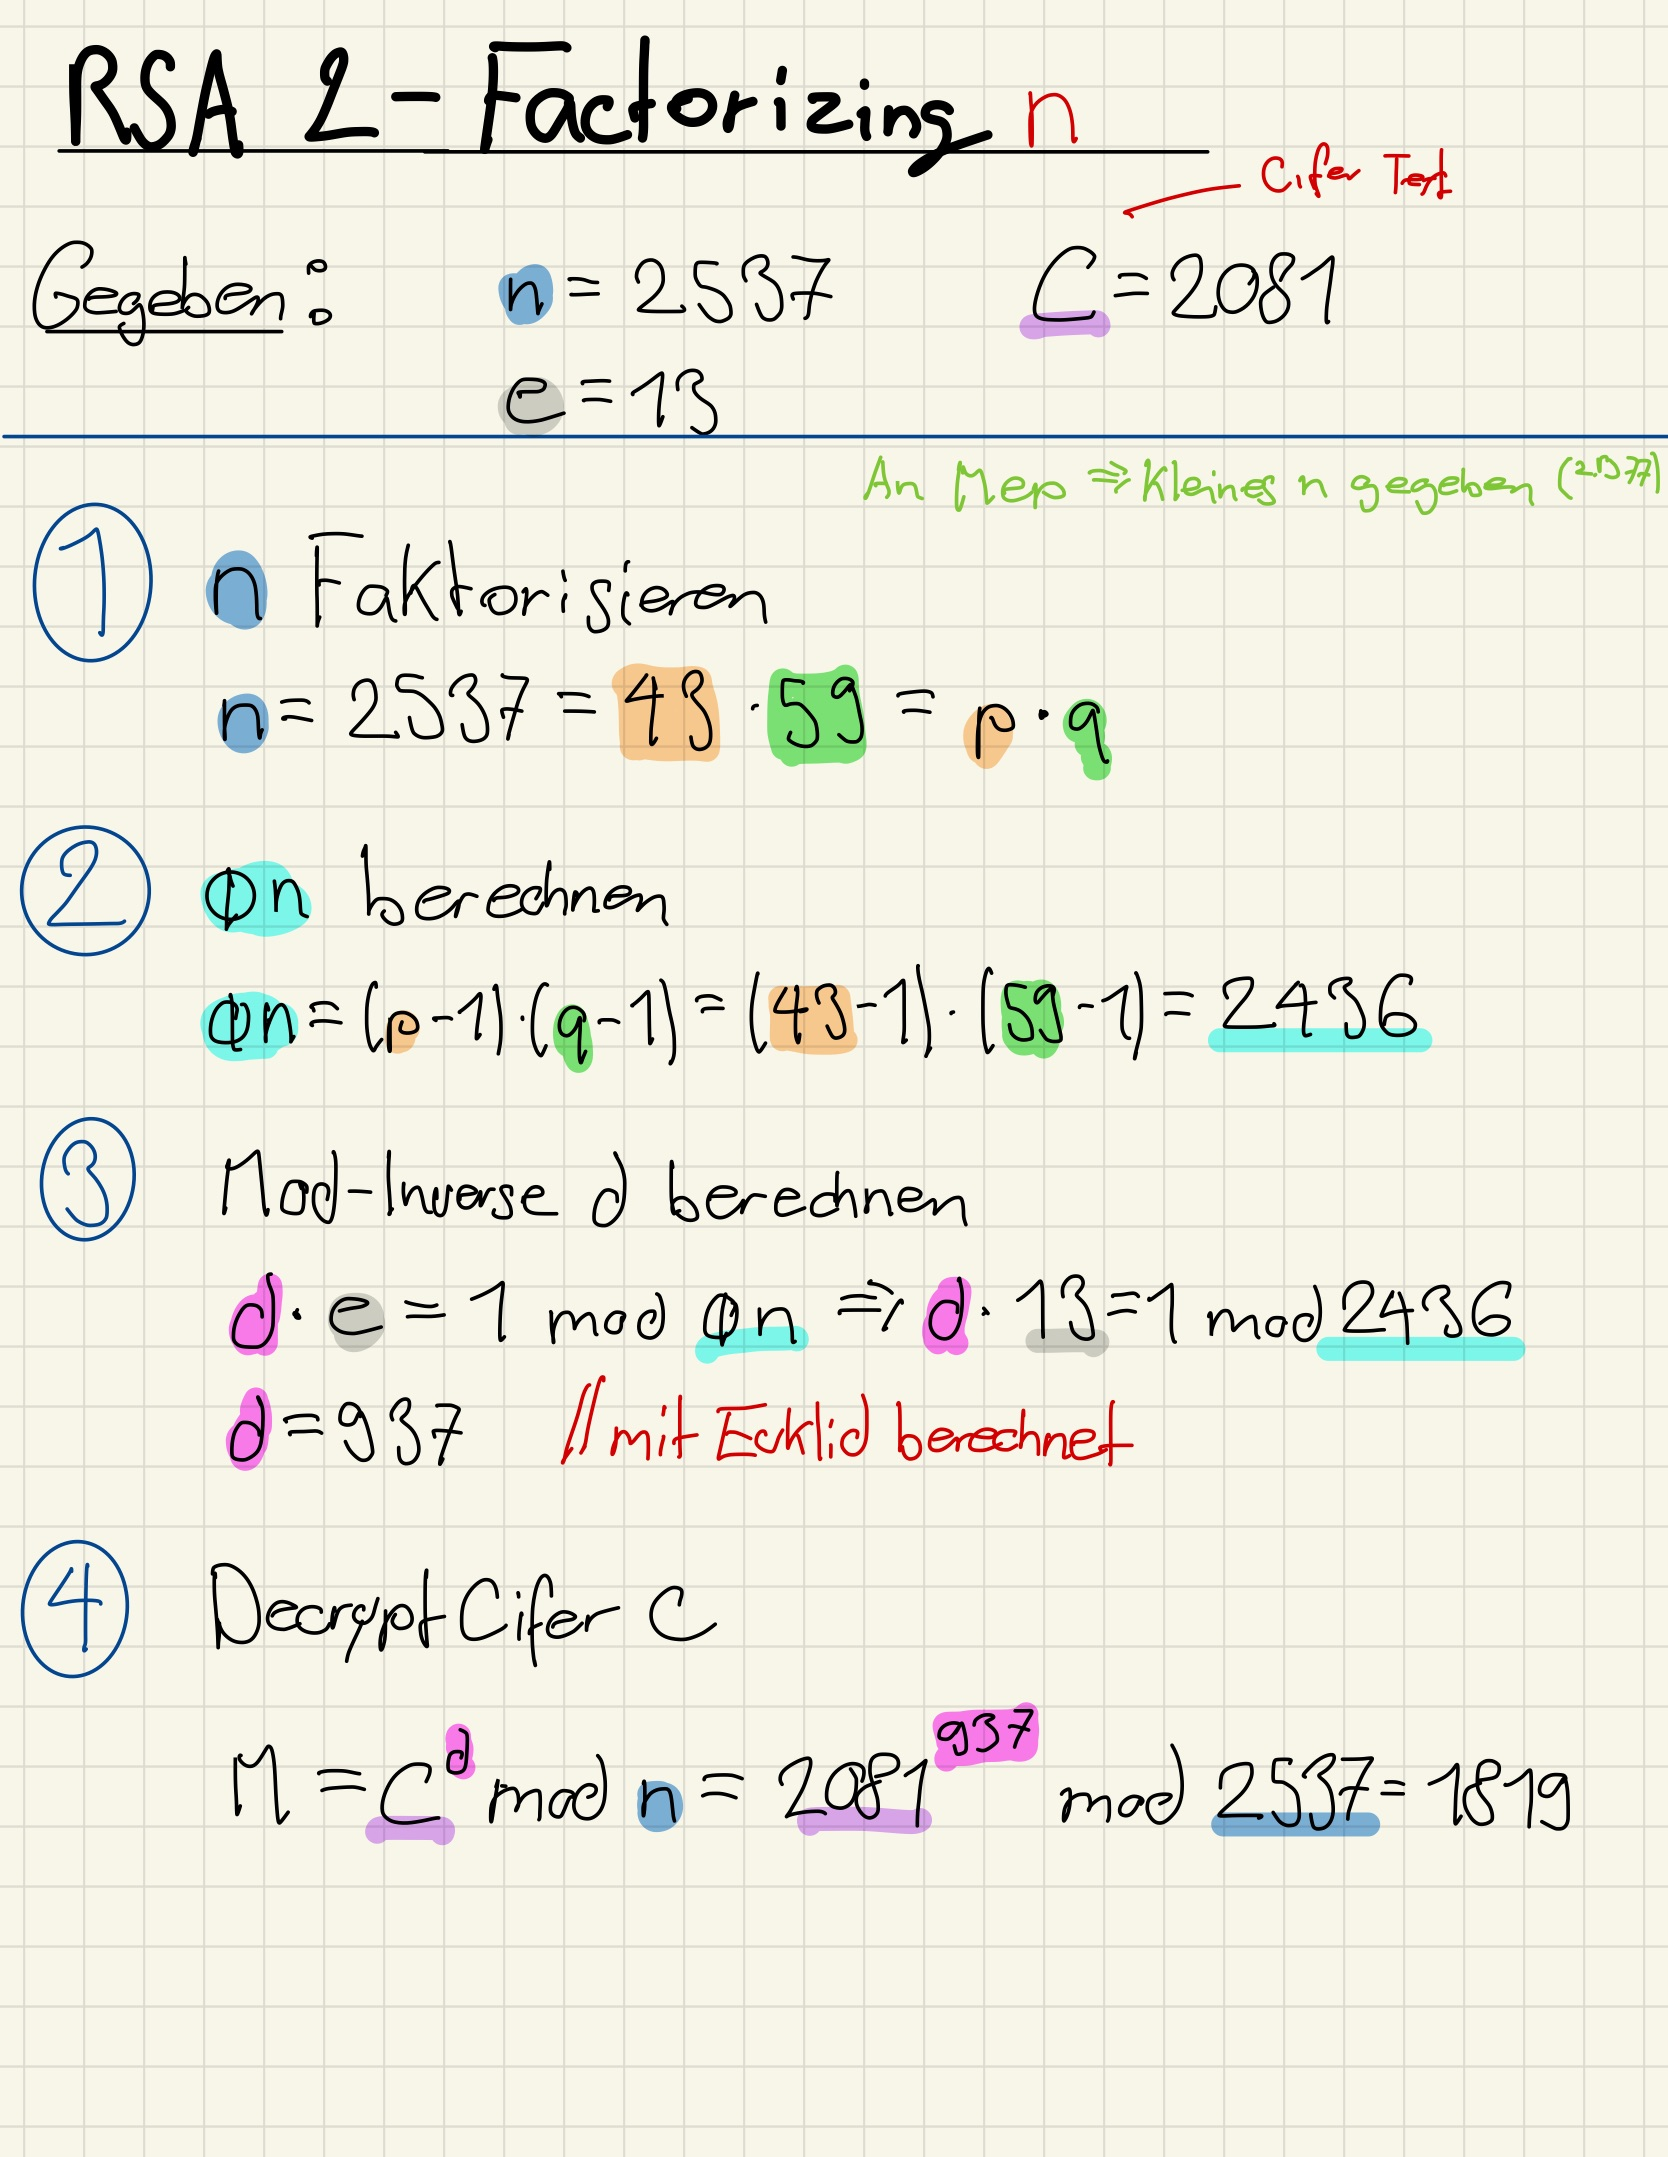
\includegraphics[scale=0.8]{img/rsa_2_factorizing.jpg}
\end{center}


    \hypertarget{attack-on-textbook-rsa-small-exponent-e}{%
\subsection{5: Attack on textbook RSA --- small exponent
e}\label{attack-on-textbook-rsa-small-exponent-e}}

Frequently, the exponent \(e\) in the public key \((n,e)\) is choosen
very small, say \(e = 3\). Hence, encryption of \(m\) is very fast

\[ c = m^3 \mod n\]

\textbf{Your Task}: Assume the message \(m\) is sent to 3 different
people using textbook RSA, with moduli \(n_1 = 377,\ n_2 = 391\), and
\(n_3 = 589\). You get hold of the corresponding ciphertexts

\[330 = m^3 \mod 377\] \[34 = m^3 \mod 391\] \[419 = m^3 \mod 589\]

Compute \(m =\sqrt[3]{x}\) using the CRT, where \(x = m^3\) satisfies
the system of linear congruences

\[ x \equiv 330 \mod 377 \] \[ x \equiv 34  \mod 391 \]
\[ x \equiv 419 \mod 589 \]

\hypertarget{solution}{%
\subsubsection{Solution}\label{solution}}

\(n_1 = 377,\ n_2 = 391\), and \(n_3 = 589\)

\(x_1 = 330 \bmod 377\), \(x_2 = 34 \bmod 391\), \(x_3 = 419 \bmod 589\)

\hypertarget{solution-steps}{%
\paragraph{Solution Steps}\label{solution-steps}}

Gegeben: n1,n2,n3 \textbar{} x1,x2,x3

\textbf{Schritt 1}

N1,N2,N3 berechnen.

\(N_1 = n_2 \cdot n_3\)\\
\(N_2 = n_1 \cdot n_3\)\\
\(N_3 = n_1 \cdot n_2\)

\textbf{Schritt 2}

y1,y2,y3 berechnen.

\(y_1 =\) mod-Inverse \(N_1 mod x_1\)\\
\(y_2 =\) mod-Inverse \(N_2 mod x_2\)\\
\(y_3 =\) mod-Inverse \(N_3 mod x_3\)

\textbf{Schritt 3}

x berechnen

x = Summe(\(x_1 \cdot N_1 \cdot\) \(y_1\) + \(x_2 \cdot N_2 \cdot\)
\(y_2\) + \(x_3 \cdot N_3 \cdot\) \(y_3\)
\(\bmod (n_1 \cdot n_2 \cdot n_3 )\))

\textbf{Schritt 4}

e-te Wurzel von x berechnen = m

\(\sqrt[3]{x} = m\)

\newpage

    \hypertarget{attack-on-textbook-rsa-common-module-n}{%
\subsection{6: Attack on textbook RSA --- common module
n}\label{attack-on-textbook-rsa-common-module-n}}

Suppose the CTO of a company wants that all employees use the same
module \(n\). The individual employees have pairwise different
\((e_i , d_i )\). Suppose, two employees \(A\) and \(B\) have the public
keys \((n,e_A)\) and \((n,e_B)\) where \(\gcd(e_A,e_B) = 1\).

Now the administration sends the encrypted message \(m\) to the two
employees

\[c_A = m^{e_A} \mod n \] \[ c_B = m^{e_B} \mod n\]

\textbf{Your Task}: Design an example with small numbers which
demonstrates, this attack!\\
Assume \(n = 11\cdot 13\), i.e. \(p = 11\) and \(q = 13\).

\hypertarget{solution}{%
\subsubsection{Solution}\label{solution}}


\begin{center}
	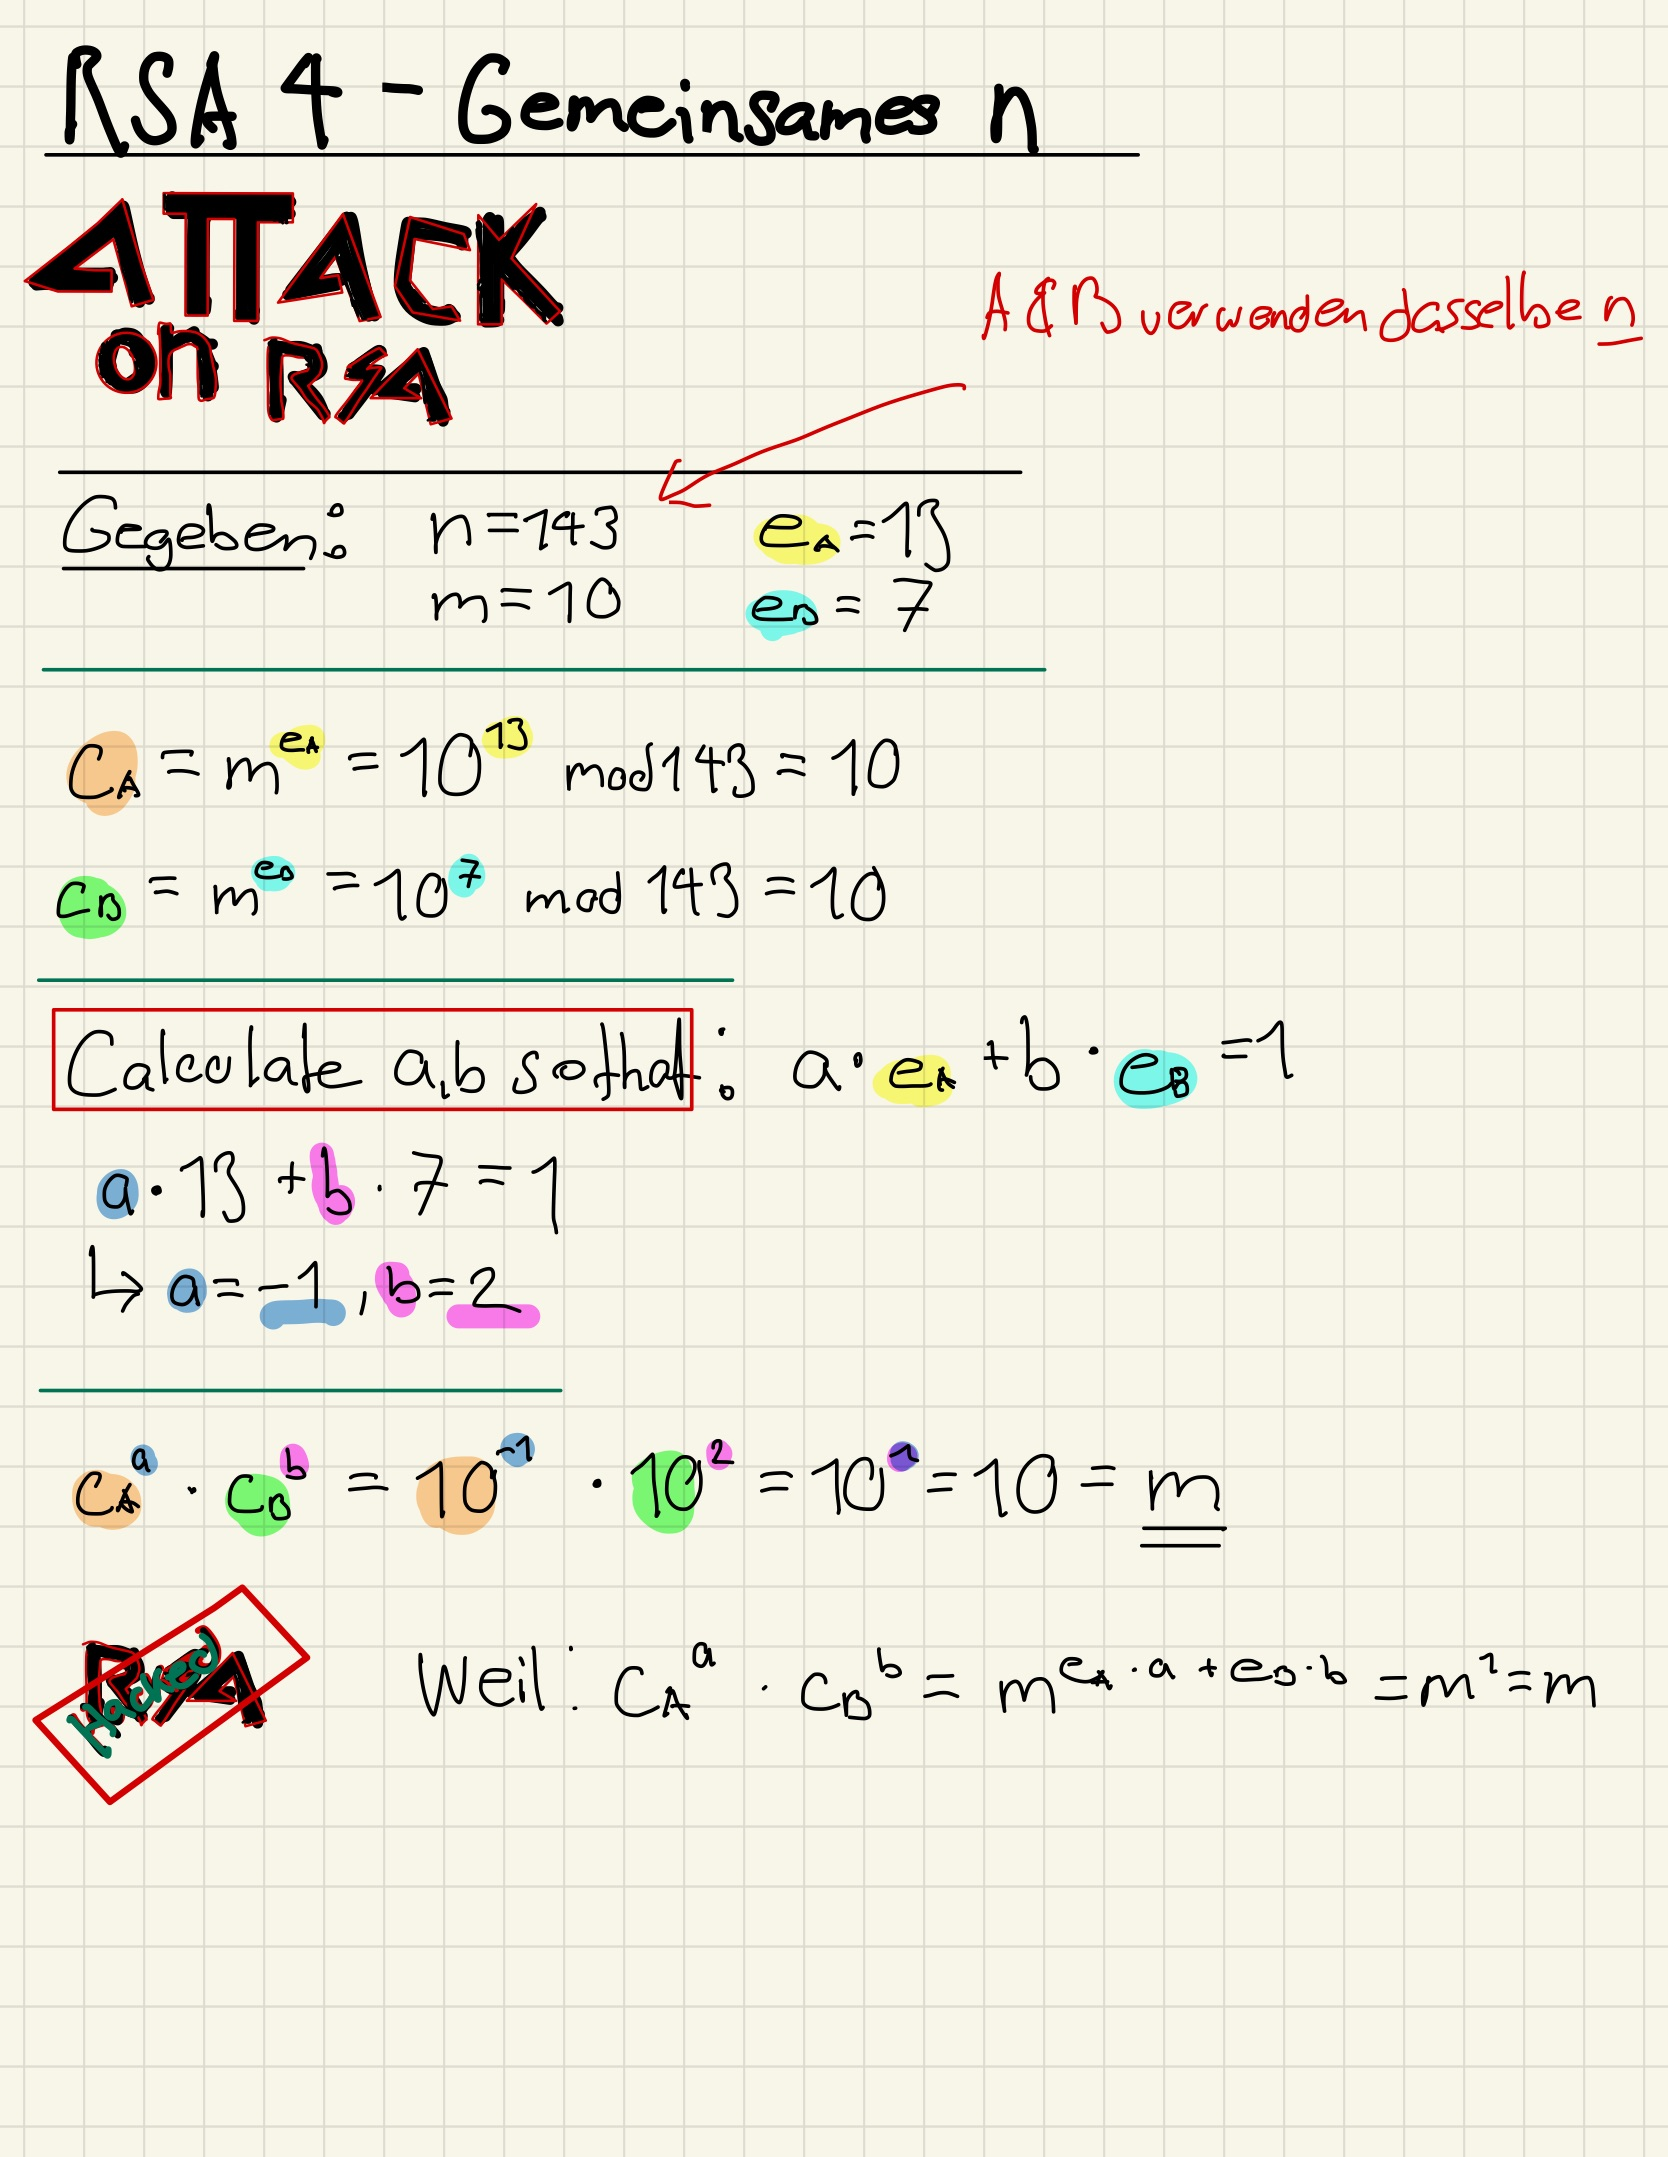
\includegraphics[scale=0.8]{img/psol5.jpg}
\end{center}

\newpage

    \hypertarget{elgamal-2nd}{%
\subsection{8: Elgamal 2nd}\label{elgamal-2nd}}

Alice uses the private key \(a=1751\) and computes the public key
\((p=2357,\alpha=2,\alpha^a =1185)\). Now Bob wants to encrypt the
message \(m = 2035\). He uses the random \(k = 1520\).

\textbf{Your Task}: Compute the encrypted message and show how Alice
decrypts the message.

\hypertarget{solution}{%
\subsubsection{Solution}\label{solution}}

\begin{center}
	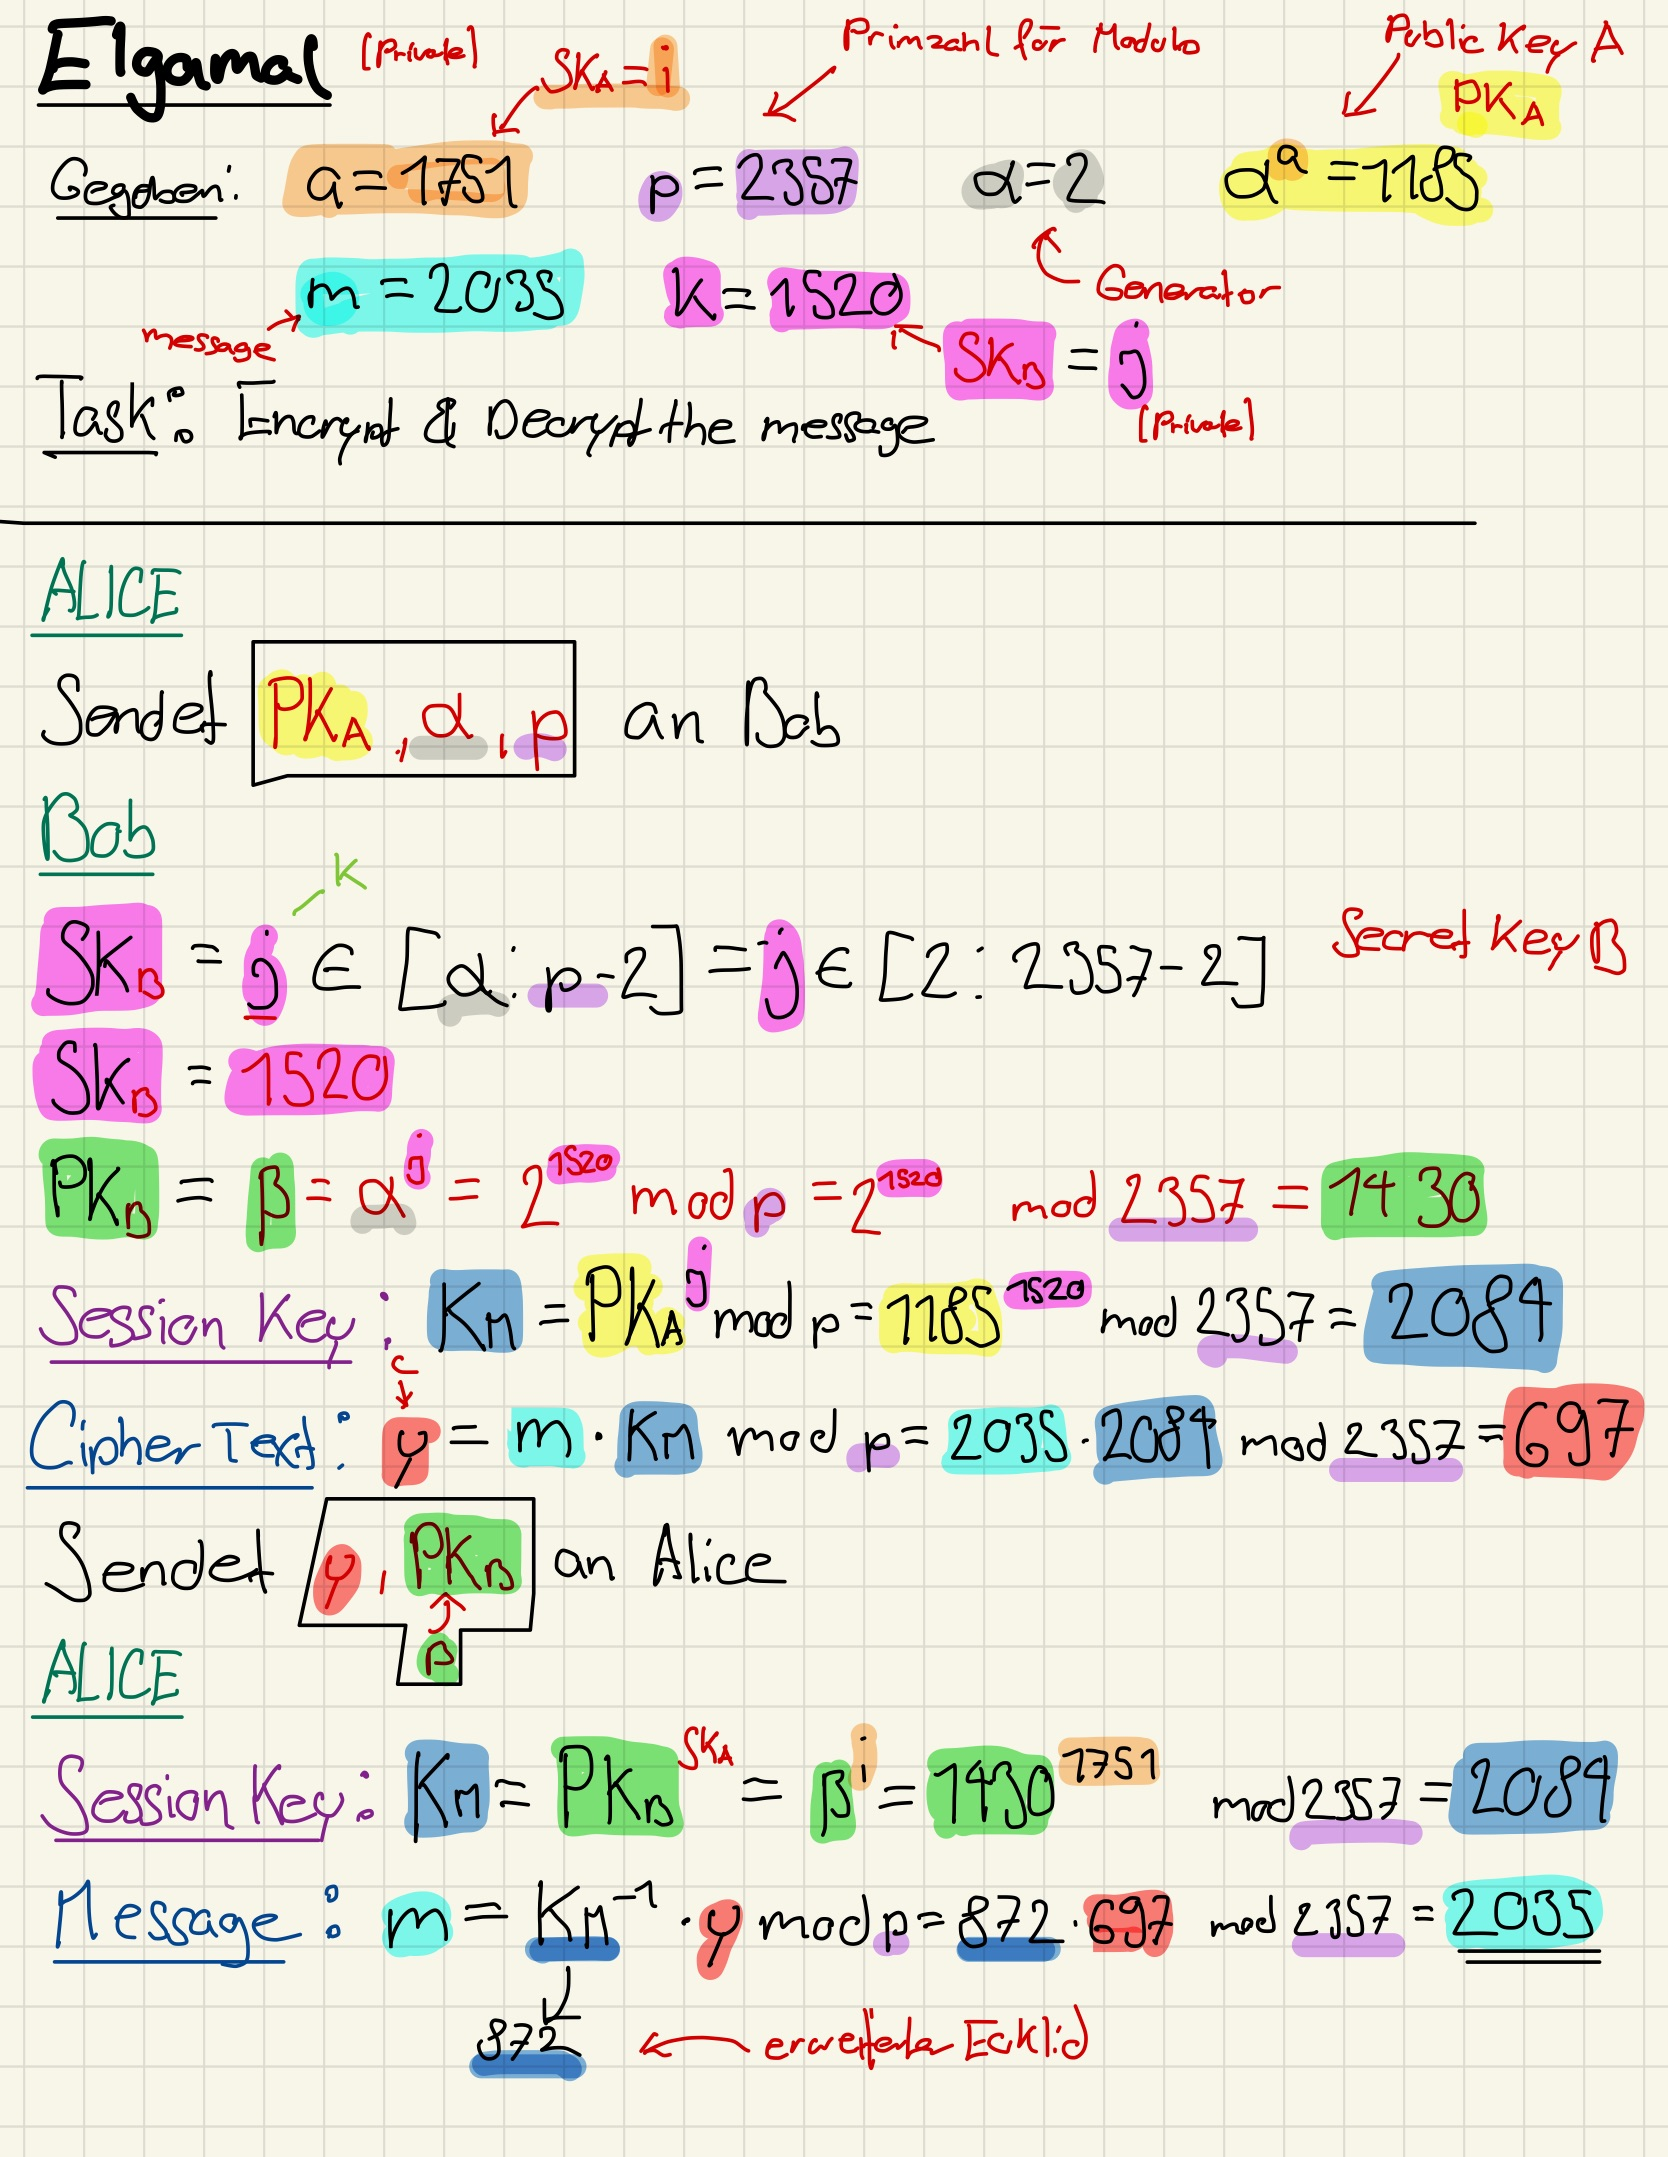
\includegraphics[scale=0.85]{img/psol6_2.jpg}
\end{center}

Der letzte Schritt \(K_{M}^{-1}\) mit erweitertem Euklid berechnen
(\(a \cdot 2084 + b \cdot 2357 = 1\))

 \newpage

\subsection{8.2: Elgamal official}\label{elgamal-official}

\begin{center}
	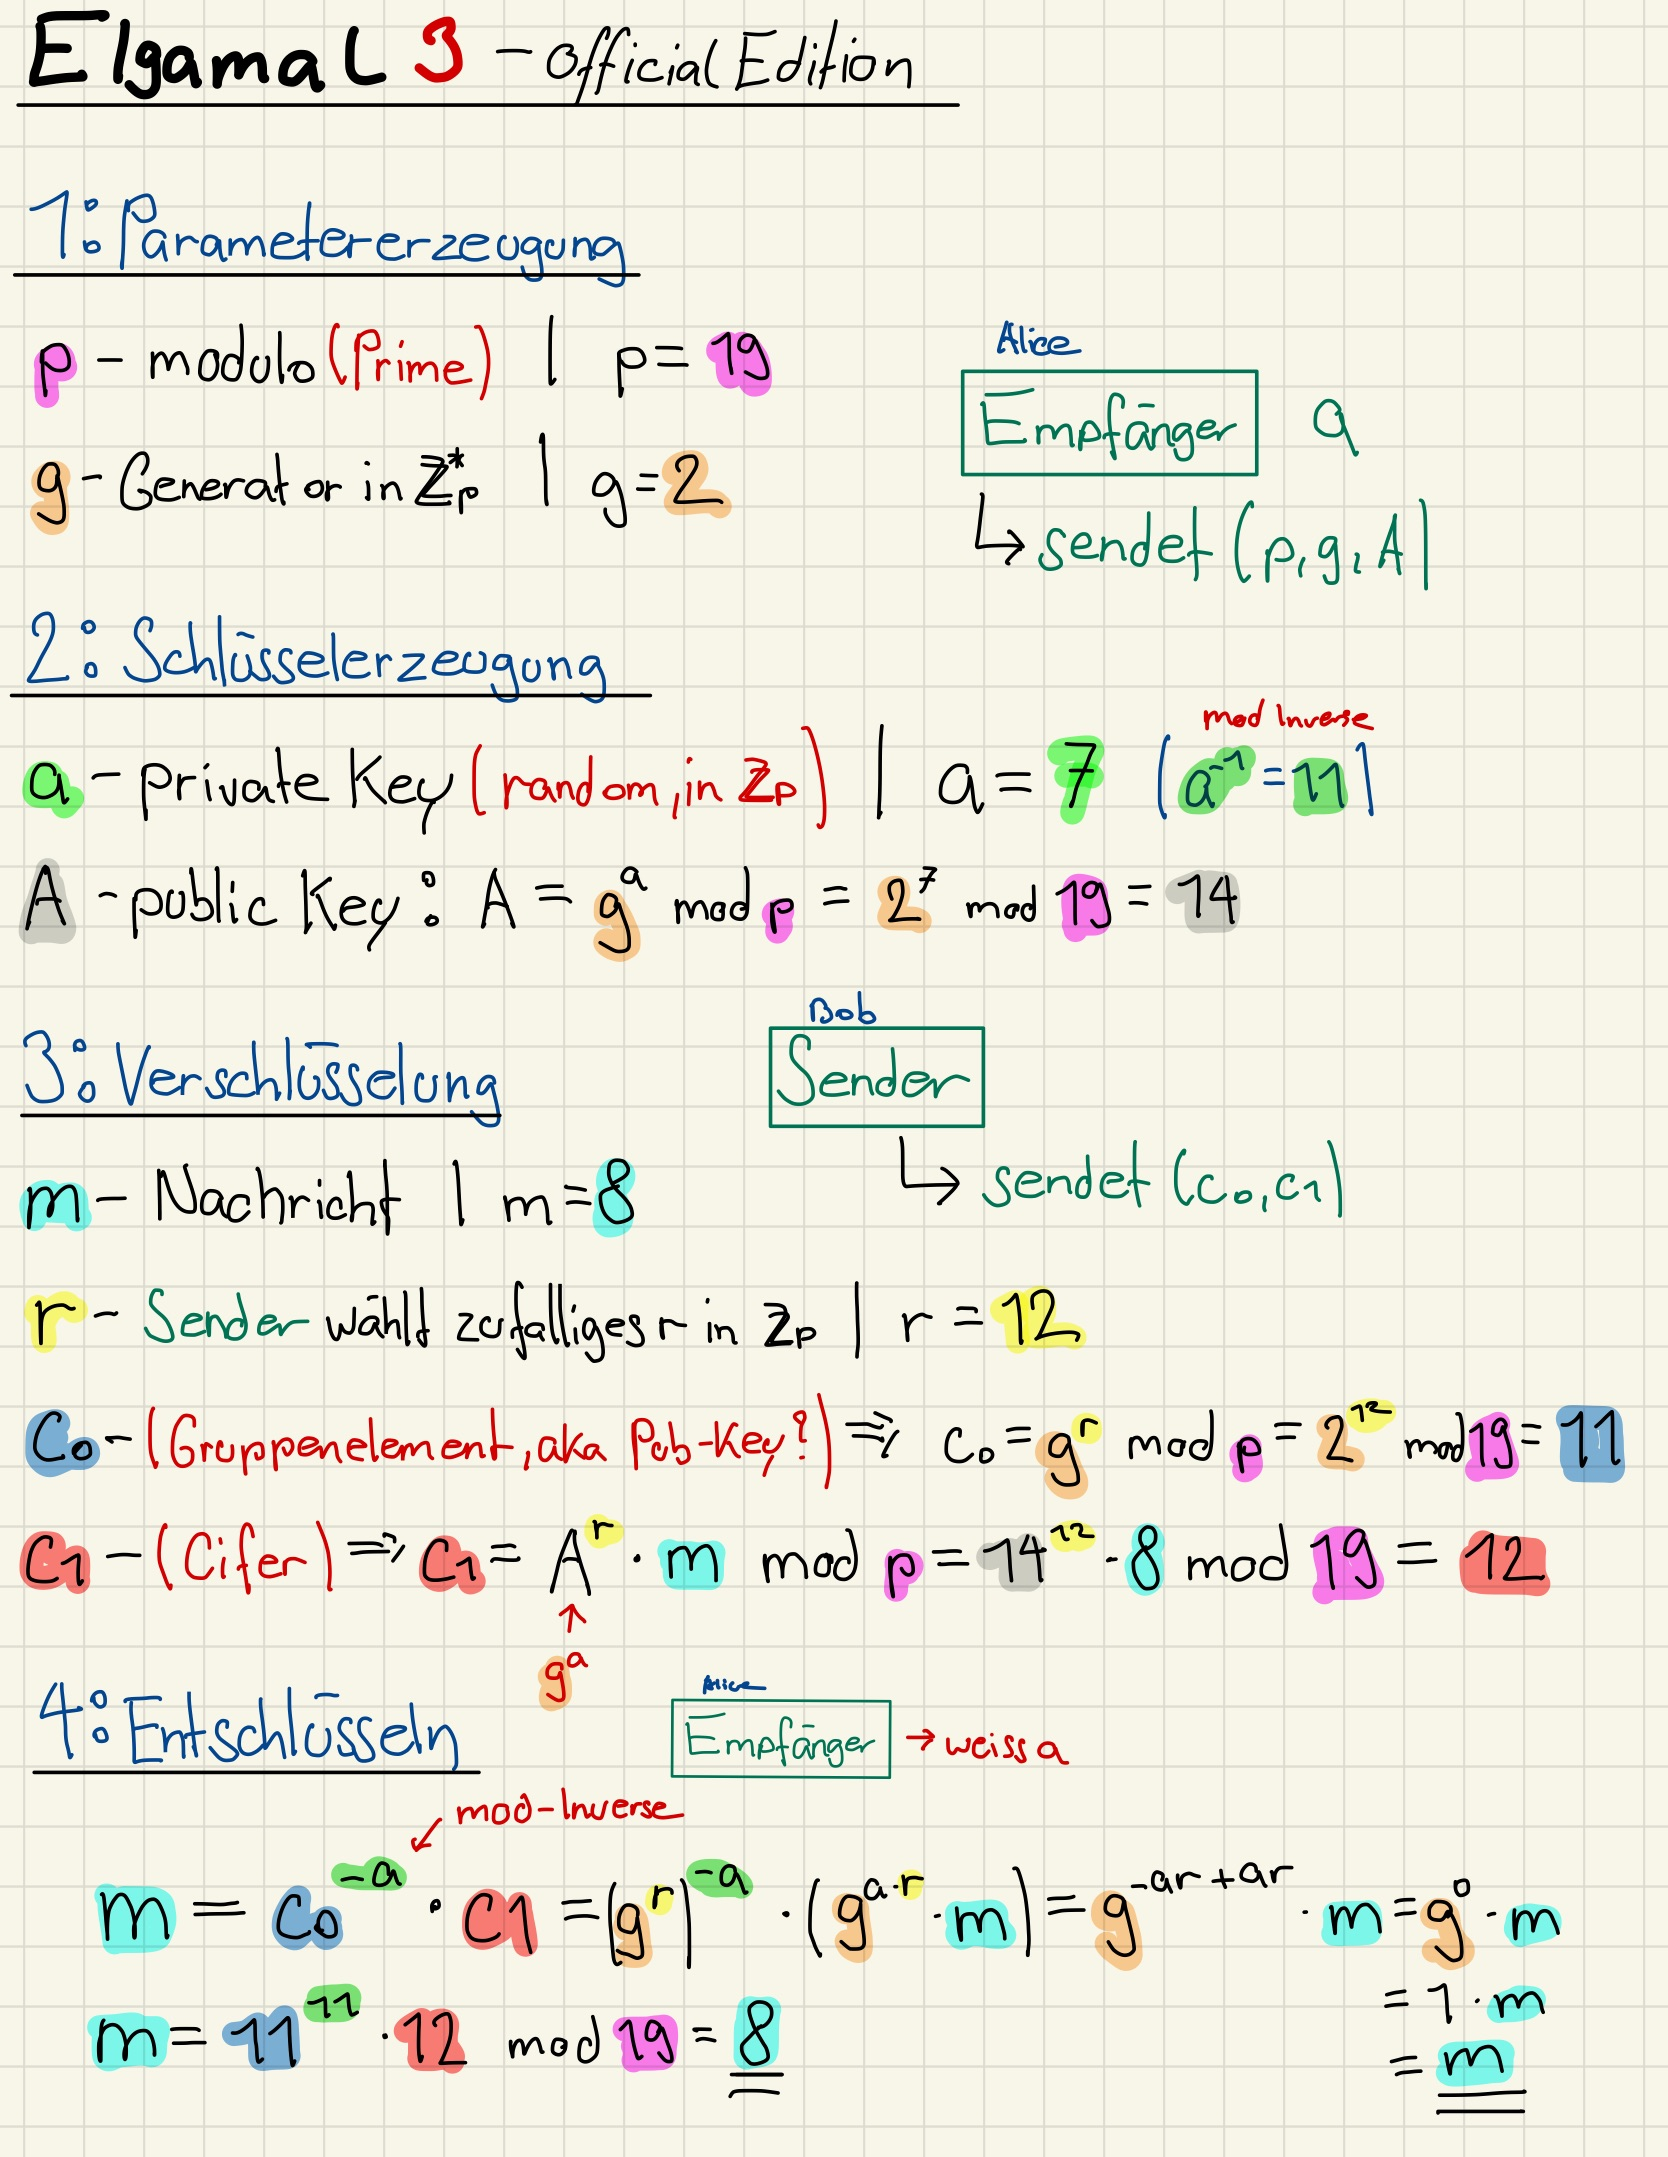
\includegraphics{img/elgamal_official.jpg}
\end{center}
 
\newpage  

    \hypertarget{sw06---public-key-cryptography-ii}{%
\section{SW06 - Public Key Cryptography
II}\label{sw06---public-key-cryptography-ii}}

    \hypertarget{elliptic-curve-over-real-numbers-mathbbr}{%
\subsection{\texorpdfstring{1: Elliptic curve over real numbers
\(\mathbb{R}\)}{1 Elliptic curve over real numbers \textbackslash{}mathbb\{R\}}}\label{elliptic-curve-over-real-numbers-mathbbr}}

Given the elliptic curve \(E : y^2 = x^3 - 3x + 9\). If this curve is
not singular (check this), compute \(a\) and \(b\), such that
\(P_1 = (0,a)\) and \(P_2 = (2,b)\) lay on \(E\). Compute
\(R = P_1 +P_2\) and draw \(E\) together with \(P_1\) , \(P_2\) and
\(R\).

\hypertarget{solution}{%
\subsubsection{Solution}\label{solution}}

\textbf{1st Step}: Always Check if its Not-Singular:

\(4a^3+27b^2 \neq 0\) (not singular)

\(4*(-3)^3+27*9^2 = -4*27 + 27*81 = 27*(81-4) \neq 0\)

\begin{center}
	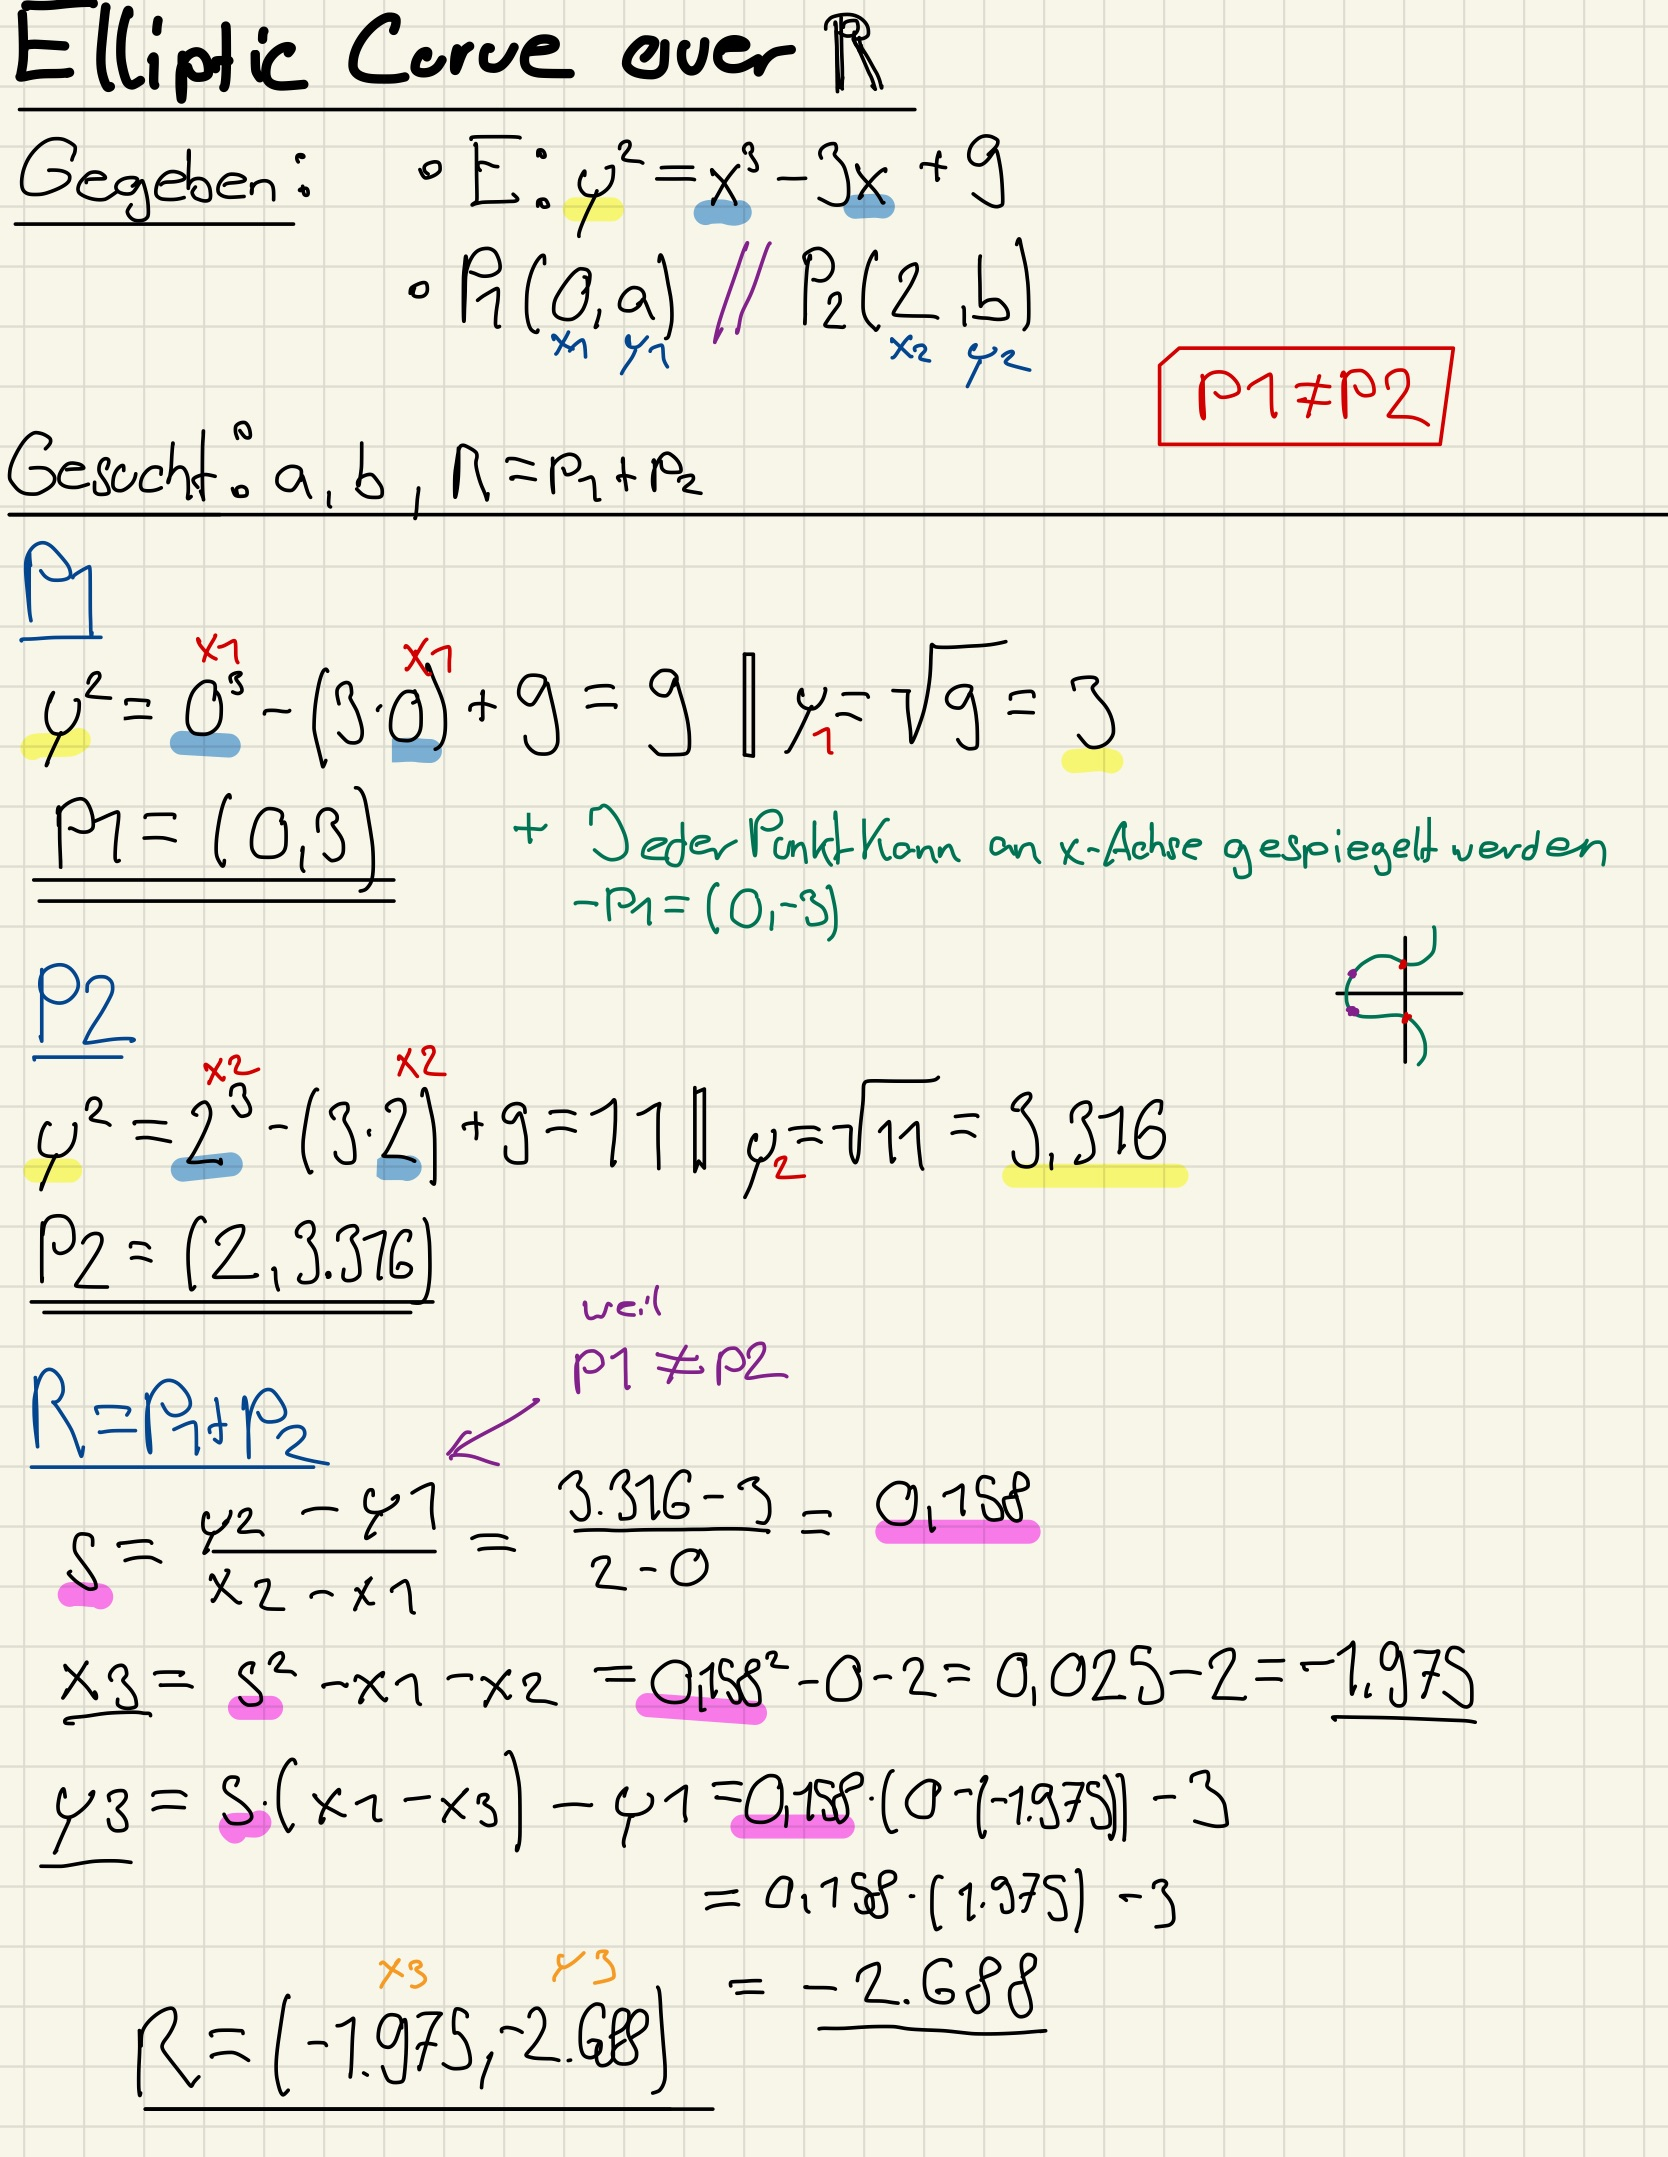
\includegraphics[scale=0.8]{img/ecurve1.jpg}
\end{center}


\newpage

    \hypertarget{elliptic-curve-over-real-numbers-mathbbr}{%
\subsection{\texorpdfstring{2: Elliptic curve over real numbers
\(\mathbb{R}\)}{2 Elliptic curve over real numbers \textbackslash{}mathbb\{R\}}}\label{elliptic-curve-over-real-numbers-mathbbr}}

Given the elliptic curve \(E : y^2 = x^3 - 3x + 5\) and point
\(P = (2,2.65) \in E\).

\textbf{Your Task}: Draw \(E\), point \(P\) and compute \(2P\), \(4P\)
and \(8P\). Solve this problem with minimal computational work!

\hypertarget{solution}{%
\subsubsection{Solution}\label{solution}}

\begin{center}
	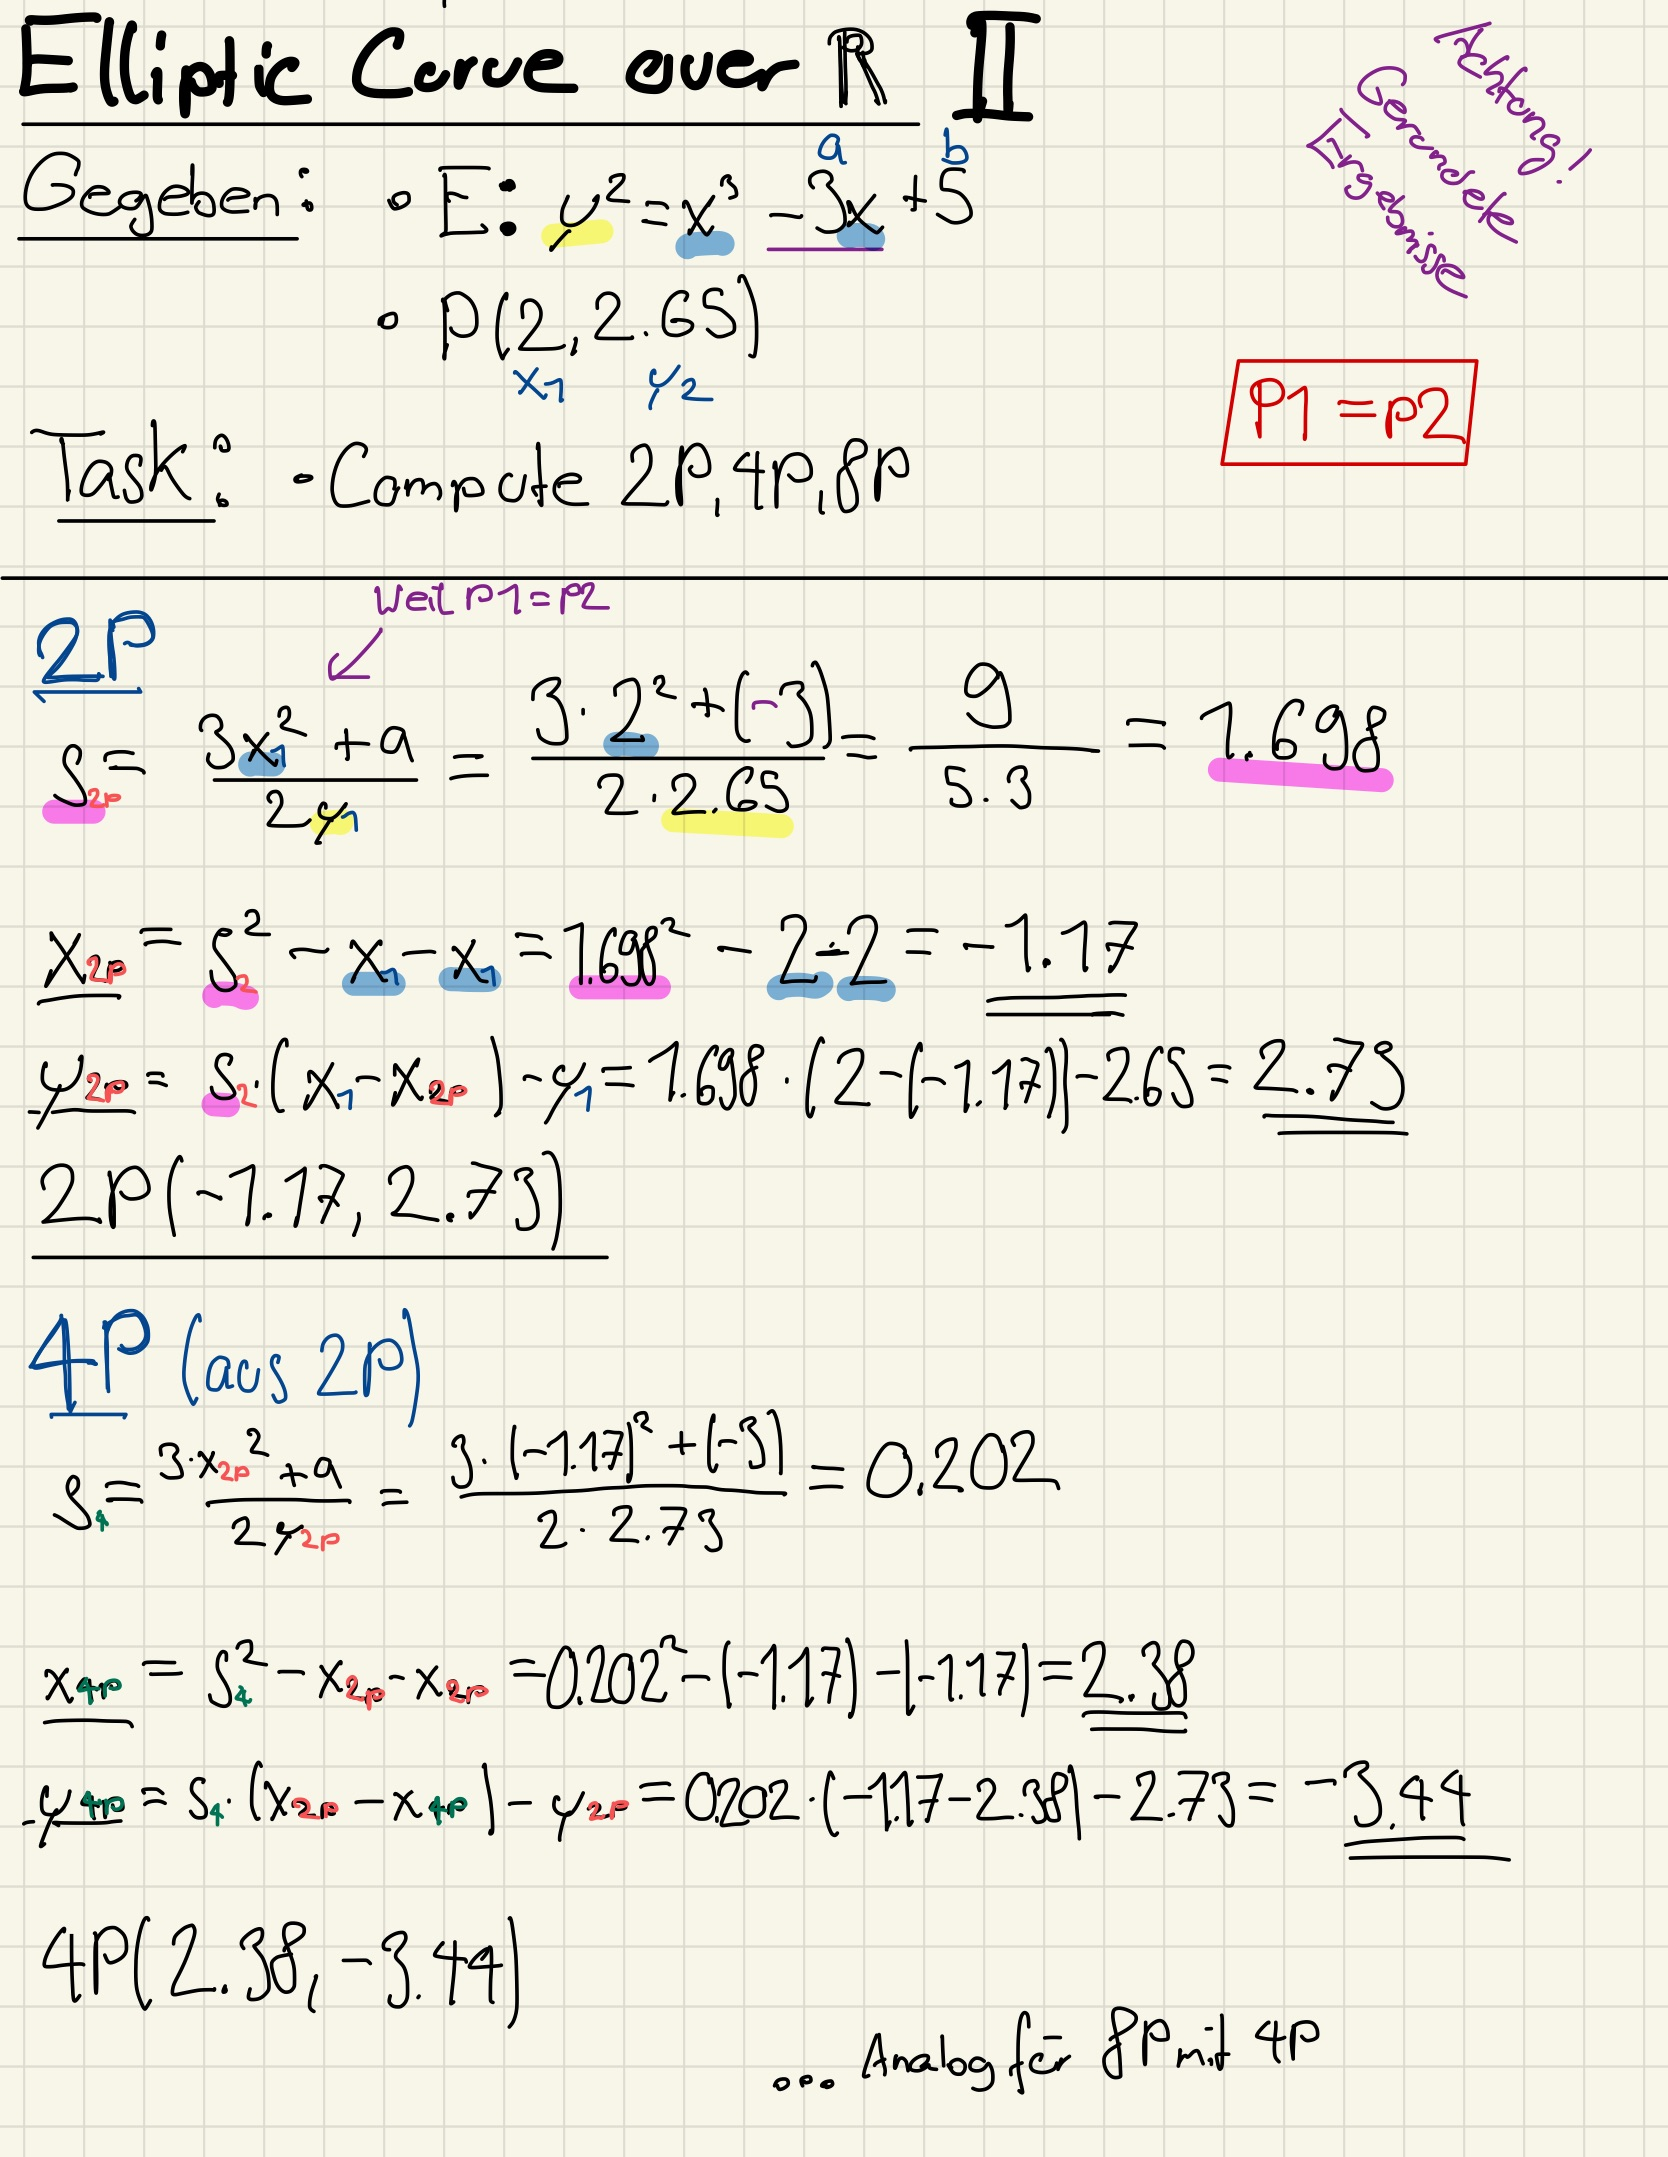
\includegraphics[scale=0.87]{img/ecurve2.jpg}
\end{center}

\newpage

    \hypertarget{elliptic-curve-over-finite-field-mathbbz_7}{%
\subsection{\texorpdfstring{4: Elliptic curve over finite field
\(\mathbb{Z}_7\)}{4 Elliptic curve over finite field \textbackslash{}mathbb\{Z\}\_7}}\label{elliptic-curve-over-finite-field-mathbbz_7}}

Let \(E : y^2 \equiv x^3 +3x+2 \bmod 7\) an elliptic curve over
\(\mathbb{Z}_7\).

\textbf{Your Task}: 1. Compute all points on \(E\) over
\(\mathbb{Z}_7\).  \\
2. What is the order of the group? (Hint: Do not miss
the identity element \(O\)) \\
3. Given the element \(\alpha = (0,3)\),
determine the order of \(\alpha\). Is \(\alpha\) a primitive element?

\hypertarget{solution}{%
\subsubsection{Solution}\label{solution}}

\begin{center}
	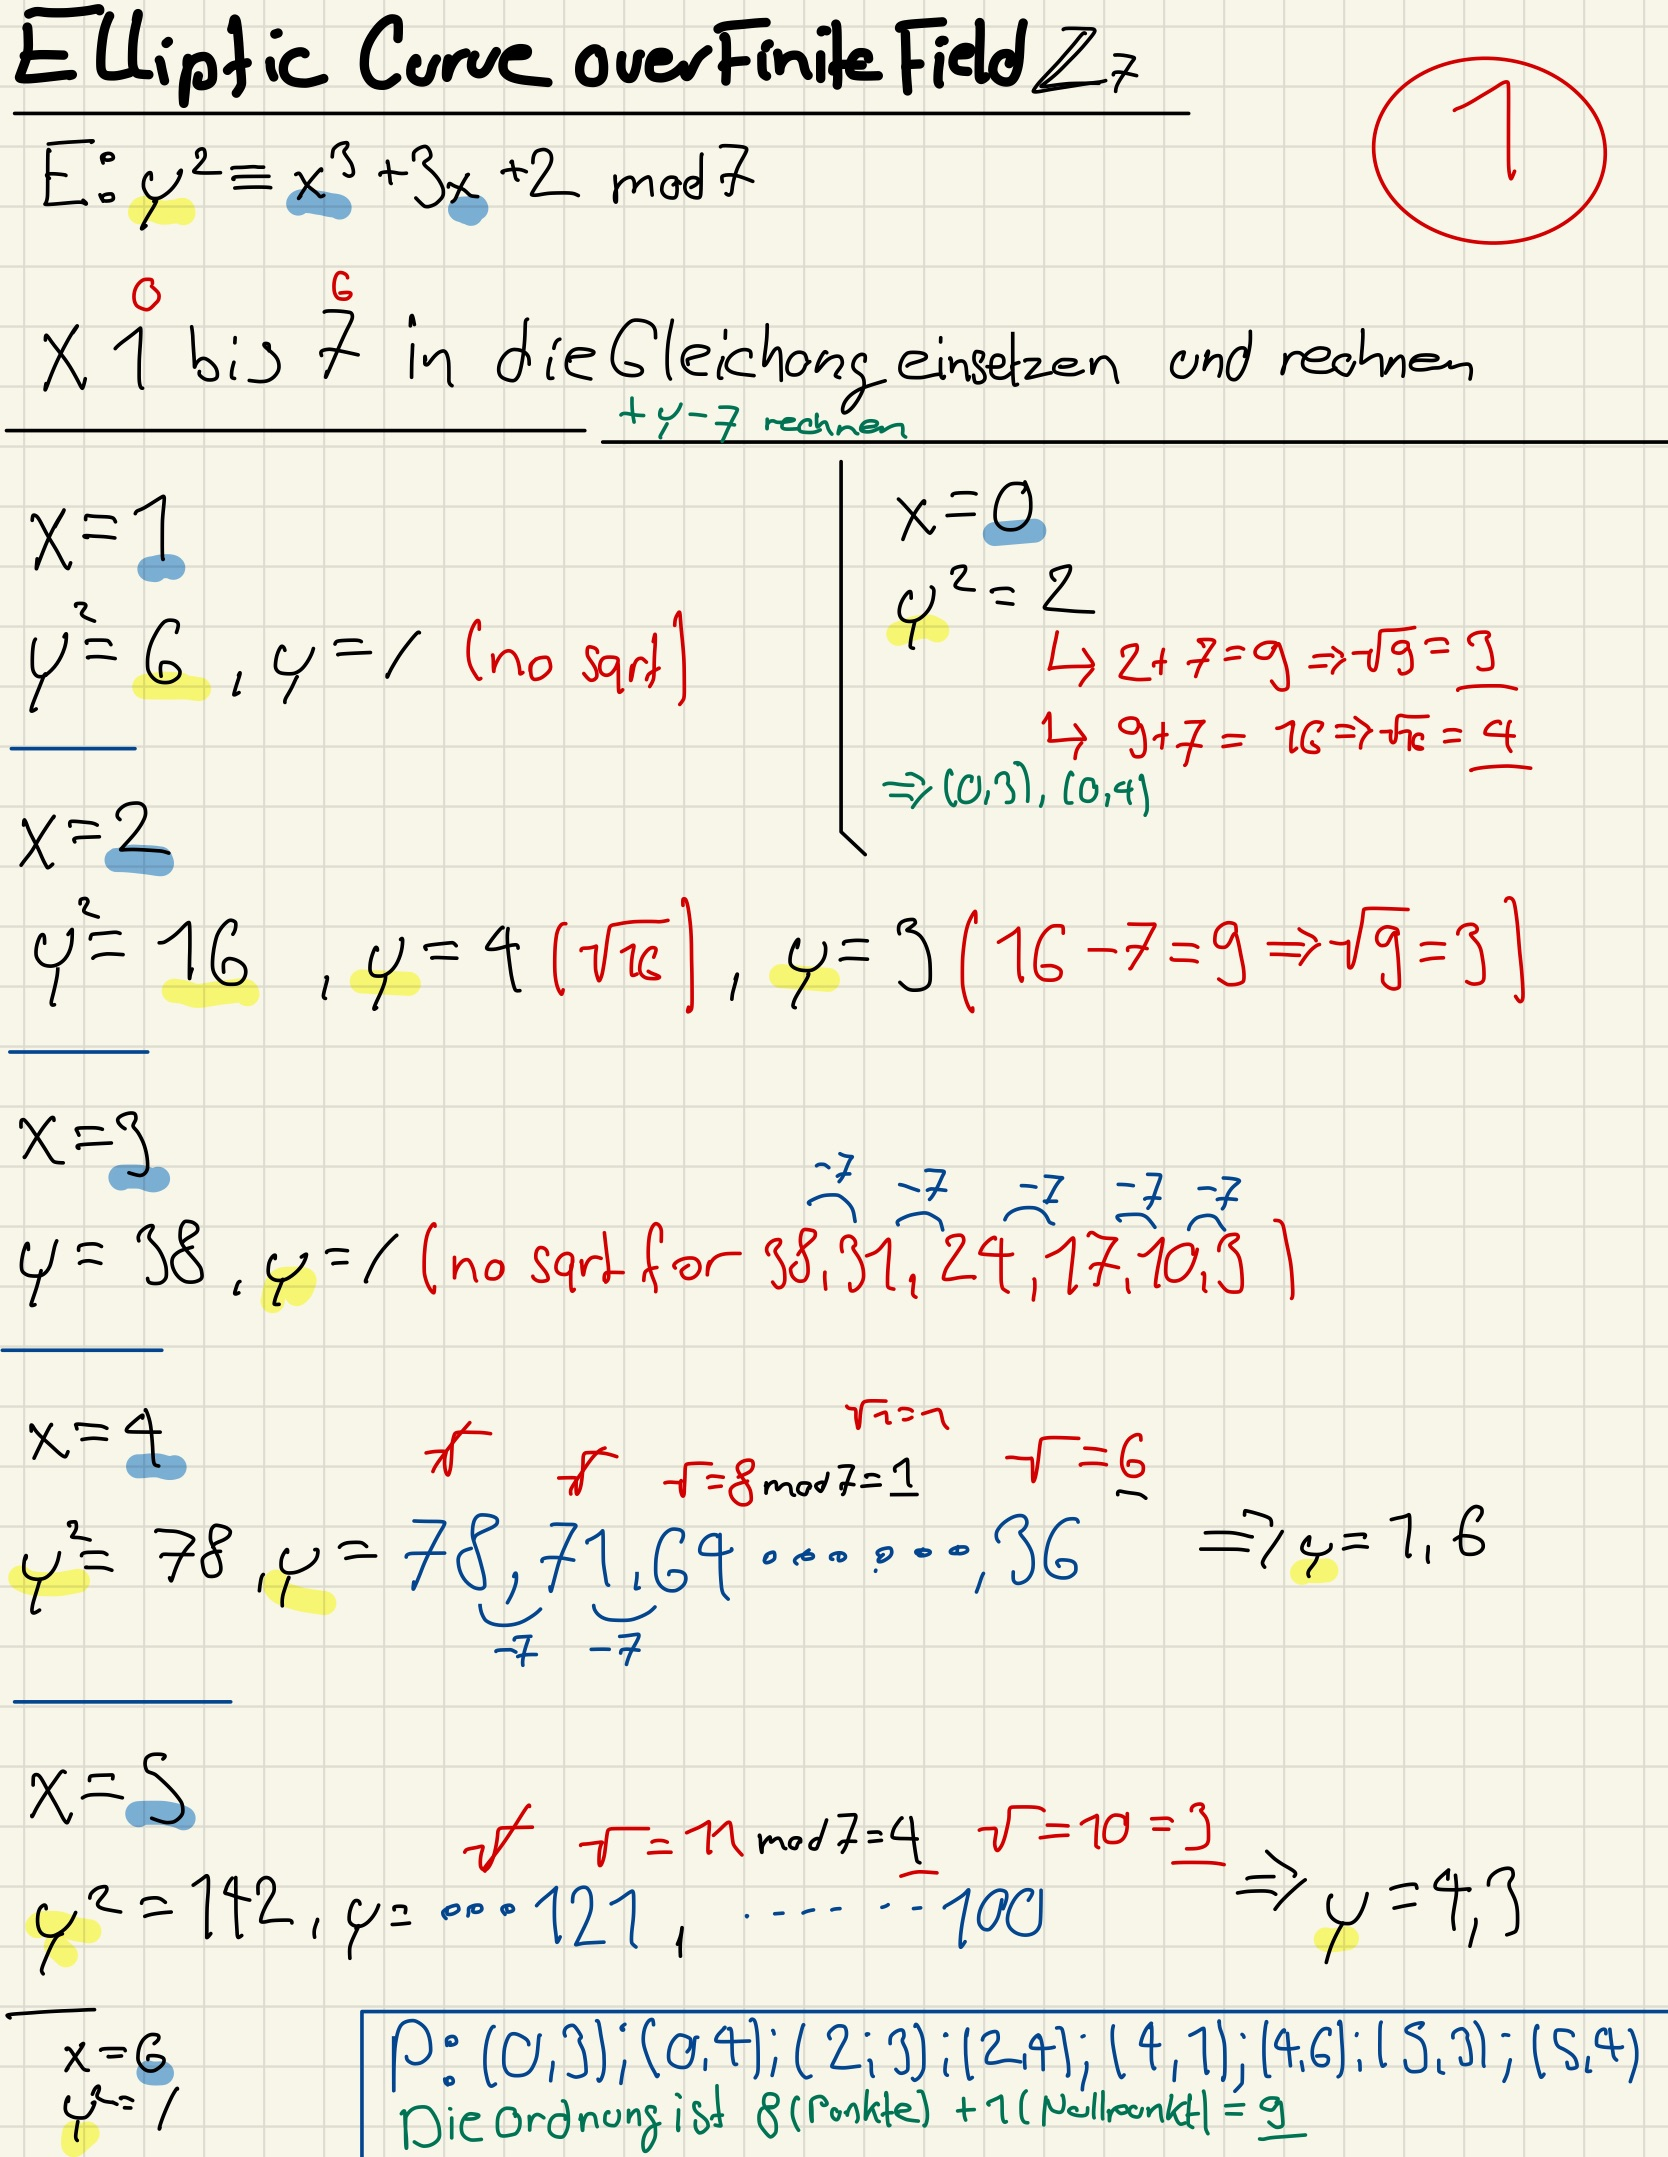
\includegraphics[scale=0.87]{img/ecurve_z_1.jpg}
	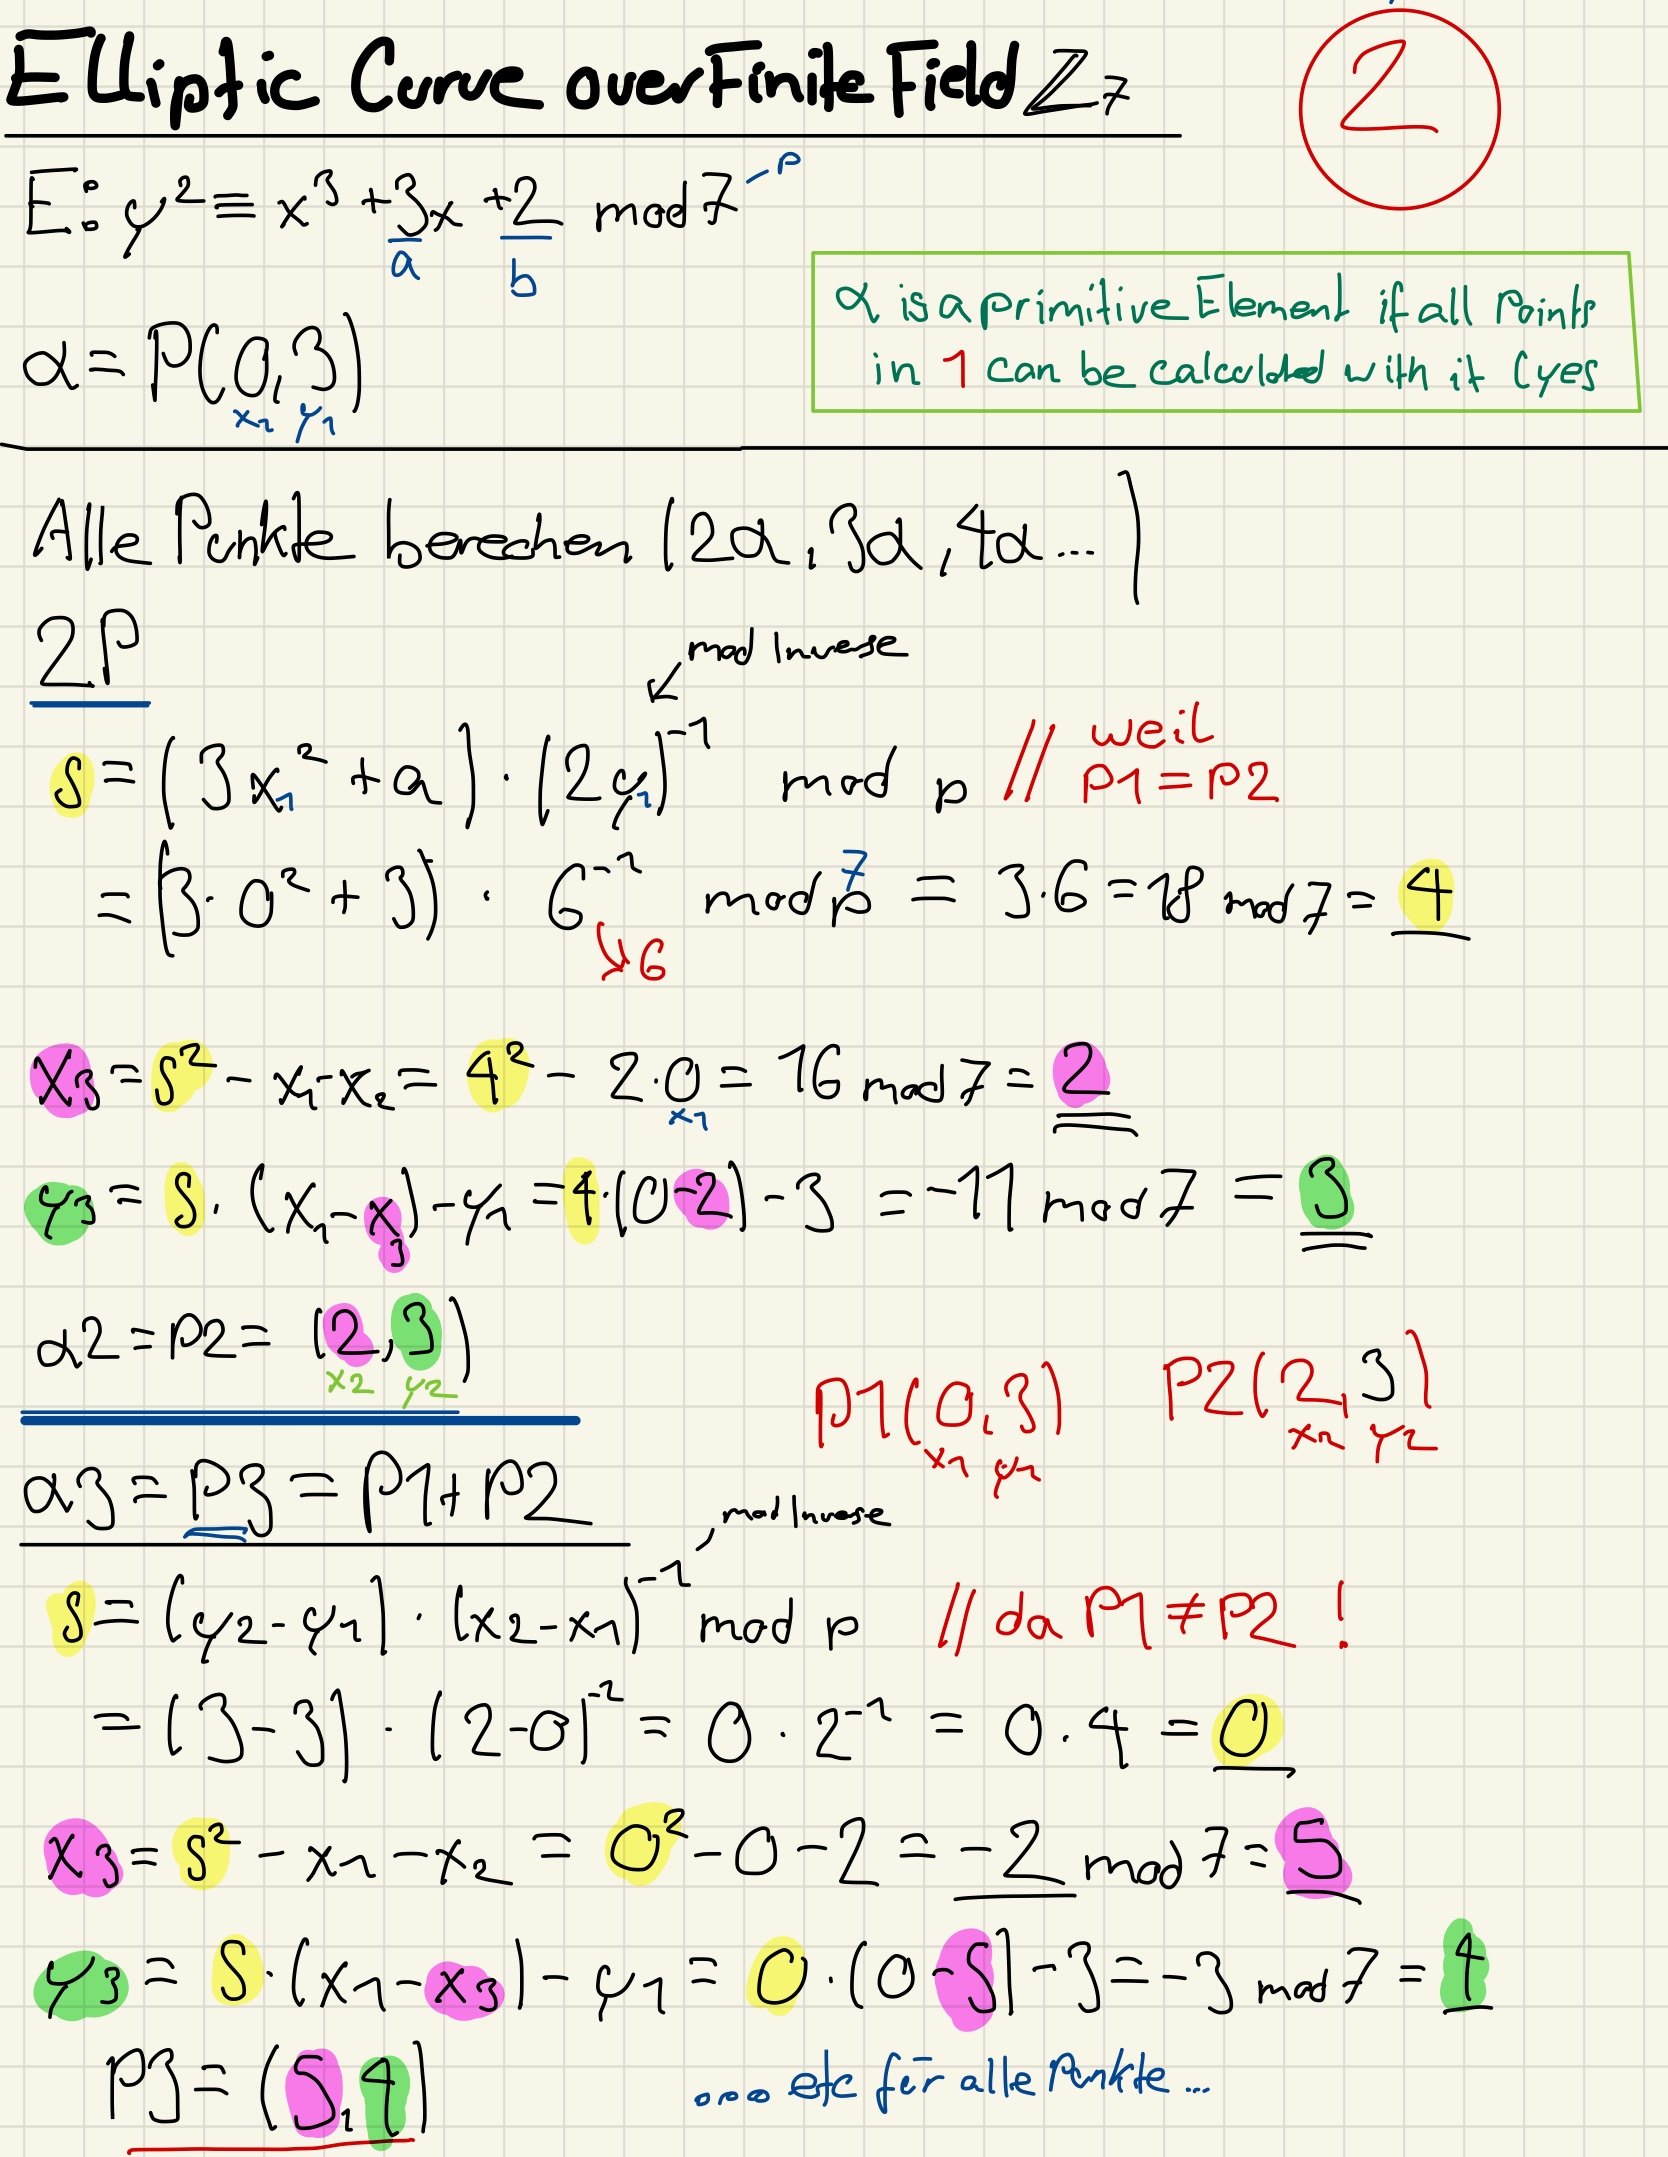
\includegraphics[scale=0.87]{img/ecurve_z_2.jpg}
\end{center}

\newpage

    \hypertarget{diffie-hellman-using-ecc}{%
\subsection{5: Diffie-Hellman using ECC}\label{diffie-hellman-using-ecc}}

Alice and Bob agree to use the elliptic curve \(E : y^2 = x^3 +x+1\) and
point \(P = (5,4) \in E\). Alice chooses her secret number \(a = 5\),
whereas Bob chooses \(b = 7\).

\textbf{Your Task}: Describe the key agreement protocol step by step
using the above assumptions about \(a\) and \(b\). What is the common
secret key?

Suppose that the elliptic curve is in mod 23 (23=n) and all points
\(\in Z\)

\hypertarget{solution}{%
\subsubsection{Solution}\label{solution}}

\(1\cdot P=(5,4)\)\\
\(2\cdot P=(17,20)\)\\
\(4\cdot P=(13,7)\)\\
\(5\cdot P=(17,3)=Q_a\)\\
\(7\cdot P\) is 0 because wether it's calculated 2P + 5P, or P + 6P, or
3P + 4P, x is always equal in both points.

\textbf{Erklärung} Da die x-Werte von (2P \& 5P), (P \& 6P), (3P \& 4P)
gleich sind, würde bei der Berechnung \(0^{-1} mod p\) rauskommen
--\textgreater{} Von 0 gibt es aber kein Modulares Inverses, weshalb 7P
= 0.

\begin{longtable}[]{@{}ll@{}}
\toprule
\begin{minipage}[b]{0.39\columnwidth}\raggedright
Alice computes \(Q_{a\cdot b} = a\cdot Q_b\)\strut
\end{minipage} & \begin{minipage}[b]{0.55\columnwidth}\raggedright
Bob computes \(Q_{a\cdot b} = b\cdot Q_a\)\strut
\end{minipage}\tabularnewline
\midrule
\endhead
\begin{minipage}[t]{0.39\columnwidth}\raggedright
\(Q_{a\cdot b} = 5\cdot Q_b\)\strut
\end{minipage} & \begin{minipage}[t]{0.55\columnwidth}\raggedright
\(Q_{a\cdot b} = 7\cdot Q_a\)\strut
\end{minipage}\tabularnewline
\begin{minipage}[t]{0.39\columnwidth}\raggedright
\(Q_{a\cdot b} = 4\cdot Q_b+Q_b\)\strut
\end{minipage} & \begin{minipage}[t]{0.55\columnwidth}\raggedright
\(Q_{a\cdot b} = 4\cdot Q_a+Q_a+2\cdot Q_a\)\strut
\end{minipage}\tabularnewline
\begin{minipage}[t]{0.39\columnwidth}\raggedright
Alice gets \(Q_{a\cdot b} = 0\)\strut
\end{minipage} & \begin{minipage}[t]{0.55\columnwidth}\raggedright
Bob gets \(Q_{a\cdot b} =0\)\strut
\end{minipage}\tabularnewline
\bottomrule
\end{longtable}

\hypertarget{kurz-erkluxe4rung-reicht-fuxfcr-mep}{%
\subsubsection{Kurz Erklärung (reicht für
MEP)}\label{kurz-erkluxe4rung-reicht-fuxfcr-mep}}

\begin{enumerate}
\def\labelenumi{\arabic{enumi}.}
\item
  Zuerst müssten mit \(1P\) alle anderen Punkte berechnet werden (2P,
  3P, 4P\ldots{} 7P) \{Dauert viel zu lange\ldots{}\}
\item
  Alice berechnet \(A\) und sendet es an Bob:
  \(A = a \cdot P = 5 \cdot P = 5P = (17,3)\)
\item
  Bob berechnet \(B\) und sendet es an Alice:
  \(B = b \cdot P = 7 \cdot P = \mathbb{O}\)
\item
  Alice kann den Common-Key berechnen:
  \(K_{BA} = a \cdot B = 5 \cdot B = 5 \cdot 7P = 35P = 5 \cdot \mathbb{O} = \mathbb{O}\)
\item
  Bob kann auch den Common-Key berechnen:
  \(K_{AB} = b \cdot A = 7 \cdot A = 7 \cdot 5P = 35P = \mathbb{O}\)
\end{enumerate}


\newpage

    \hypertarget{elliptic-curve-discrete-logarithm-problem-ecdlp}{%
\subsection{6: Elliptic Curve Discrete Logarithm Problem
(ECDLP)}\label{elliptic-curve-discrete-logarithm-problem-ecdlp}}

Assume Mallory intercepts the message \(A = (10,6)\) from Alice to Bob
and \(B = (7,11)\) from Bob to Alice. He also knows the elliptic curve
\(E : y^2 \equiv x^3 +2x+2 \bmod 17\), which forms a cyclic group of
order 19, and point \(P = (5,1)\).

\textbf{Your Task}: Suppose Mallory wants to know the common key.
Describe his steps to find this key!

\hypertarget{solution}{%
\subsubsection{Solution}\label{solution}}

\begin{center}
	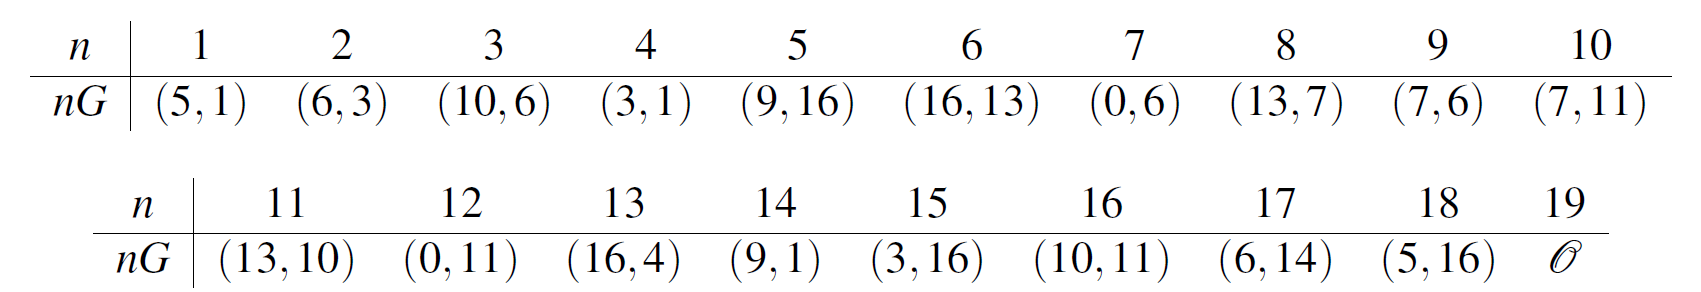
\includegraphics[scale=0.8]{img/p19Tabelle.png}
\end{center}

\hypertarget{kurzbeschreibung-fuxfcr-mep}{%
\paragraph{Kurzbeschreibung (für
MEP)}\label{kurzbeschreibung-fuxfcr-mep}}

\begin{enumerate}
\def\labelenumi{\arabic{enumi}.}
\item
  Mit der Kurvenformel und P1 alle anderen Punkte bis P19 berechnen.
  (dauert wieder ewigs)
\item
  In der Tabelle schauen, welche P's den Punkten \(Alice: (10,6)\) und
  \(Bob: (7, 11)\) entsprechen -\textgreater{} P3 und P10
\item
  Voila: Secret Key Alice=3, Bob=10
\end{enumerate}

    

    \hypertarget{sw07---protokolle-i-ladan}{%
\section{SW07 - Protokolle I (Ladan)}\label{sw07---protokolle-i-ladan}}

    \hypertarget{diffie-hellmann-schluxfcsselaustausch}{%
\subsection{1:
Diffie-Hellmann-Schlüsselaustausch}\label{diffie-hellmann-schluxfcsselaustausch}}

Im Unterricht wurde das Protokoll Diffie-Hellmann sicher vorgeführt.
Kann ein Angreifer\\
Namens Mr.~X das System angreifen, falls er die Zahlen \(\alpha\) und
\(\beta\) kennen würde? Begründen Sie\\
Ihre Antwort.

\hypertarget{solution}{%
\subsubsection{Solution}\label{solution}}

\(\alpha\) und \(\beta\) sind A und B , sprich die öffentlichen Teile
des Schlüssels.\\
Das Knacken des Diffie-Hellmann-Schlüsselaustauschprotokolls ist
gleichwertig zum Berechnen des diskreten\\
Logarithmus und somit nicht in vernünftiger Zeit lösbar.

\newpage

    \hypertarget{blinde-signatur}{%
\subsection{3: Blinde Signatur}\label{blinde-signatur}}

Führen Sie zu Zweit die blinde Signatur durch. Protokollieren Sie das
Vorgehen und zeigen Sie, wie der Signierer die Nachricht berechnen kann,
welche er (blind) signiert!

\hypertarget{solution}{%
\subsubsection{Solution}\label{solution}}

\begin{center}
	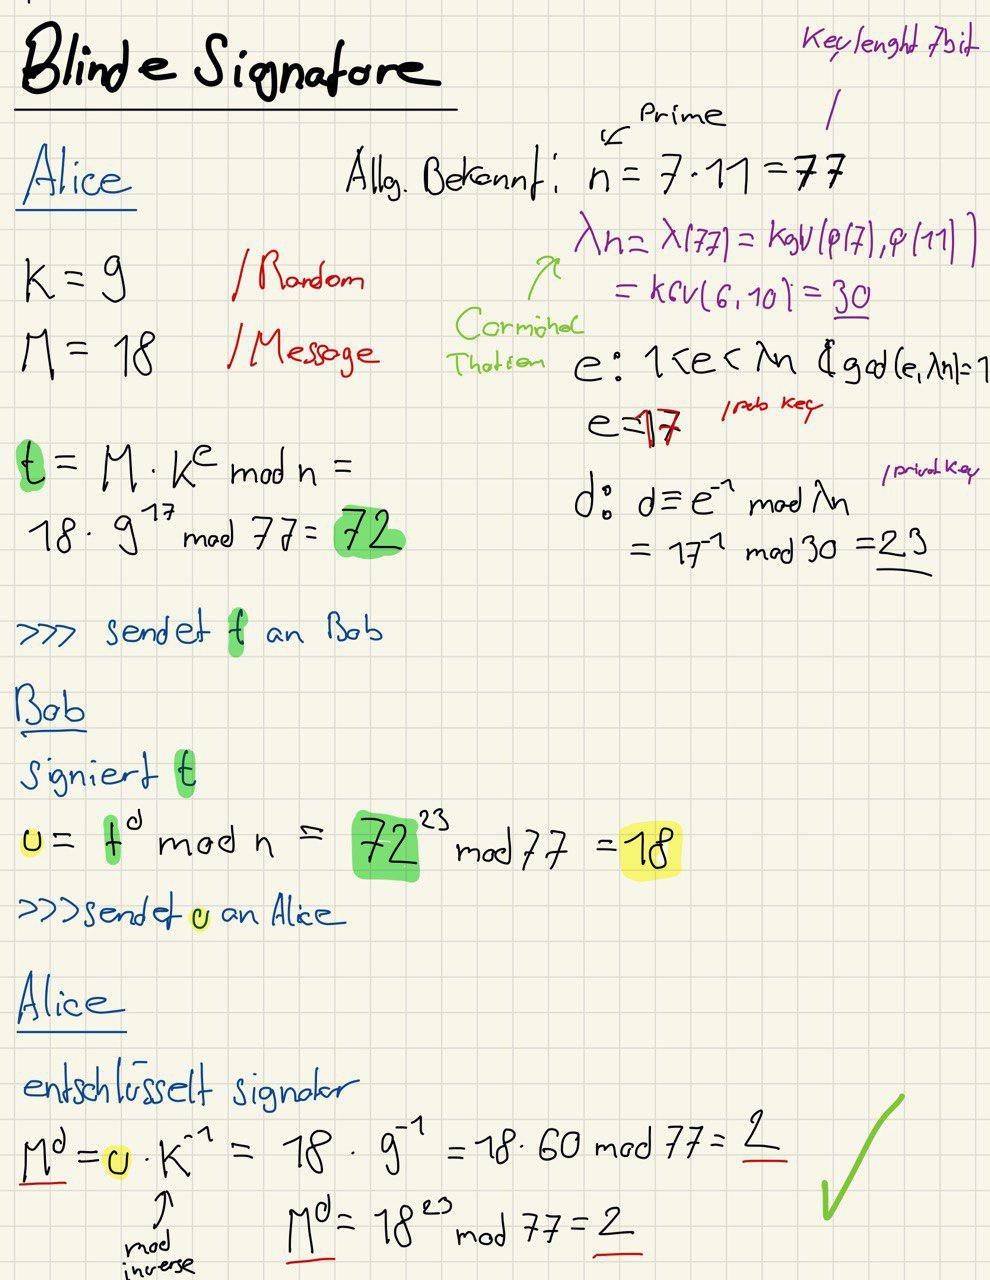
\includegraphics[scale=0.85]{img/blindsig.jpg}
\end{center}

\textbf{INFO}: \(\Delta\) n habe ich hier mit kgv berechnet, das ist
nicht falsch (die Rechnung geht auf) aber für das wahre RSA und für
unsere Prüfung müssen wir phi(n) --\textgreater{} Also (p-1)*(q-1)
verwenden. Hier die phi(n) Variante:

\begin{center}
	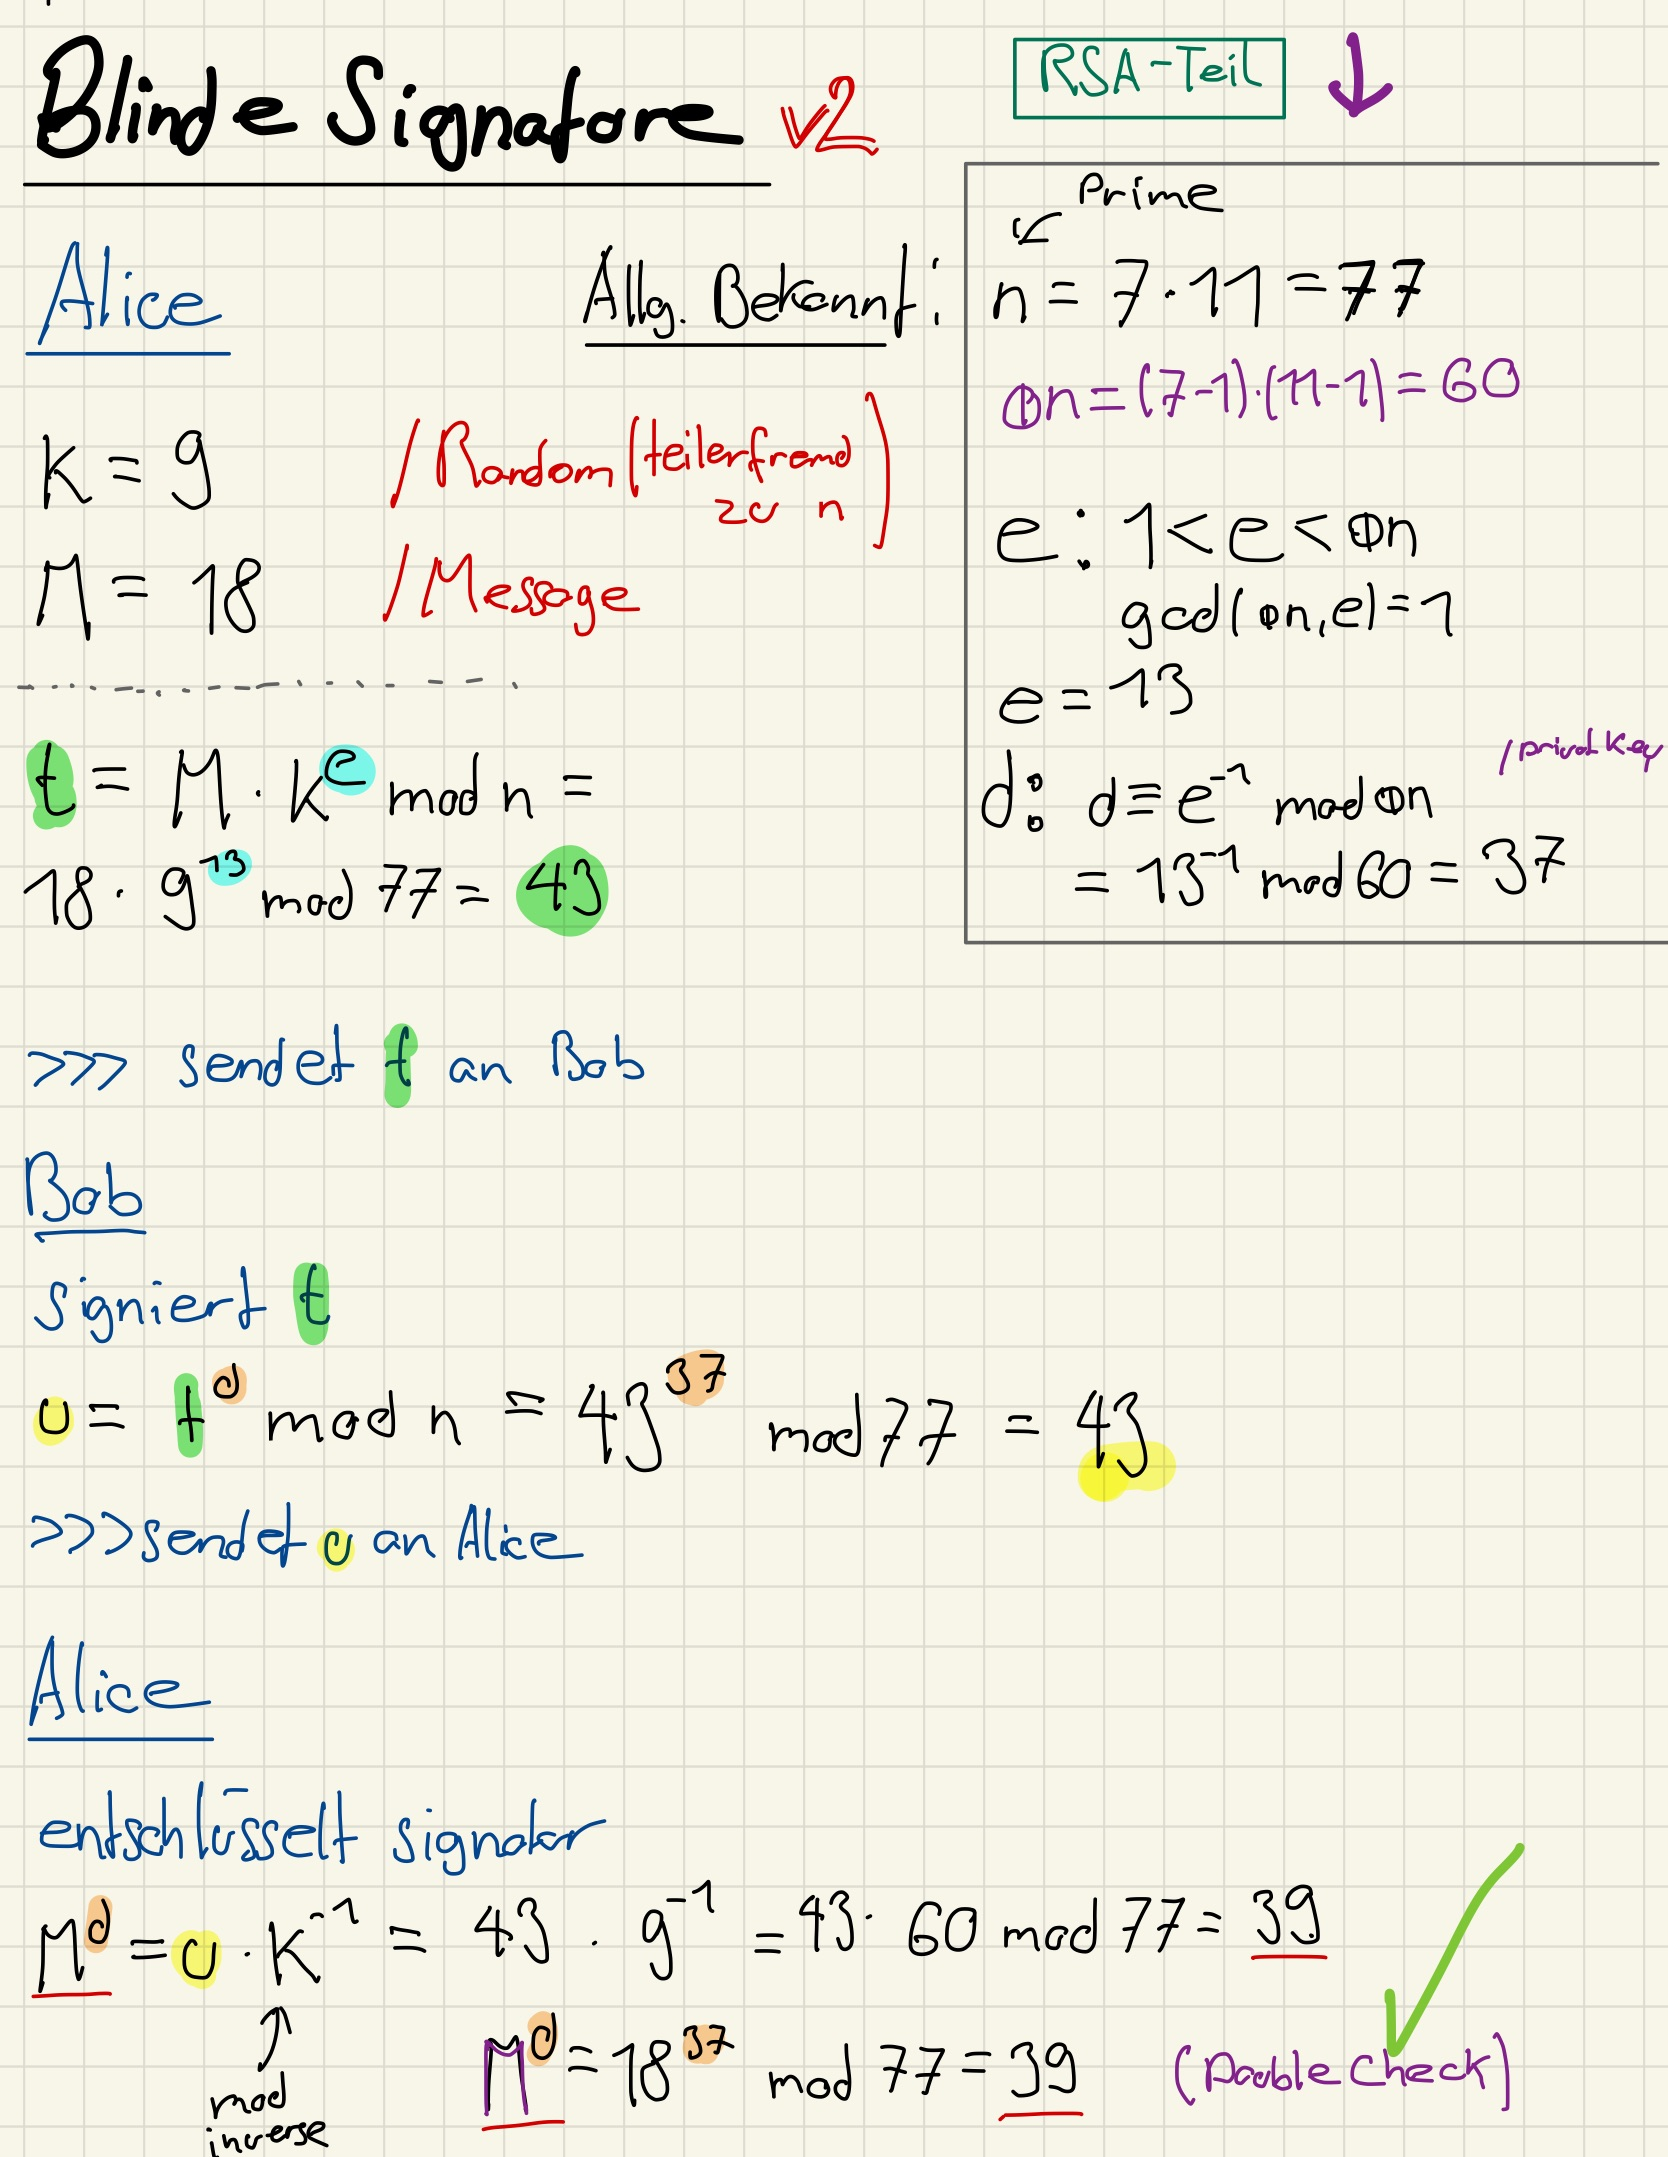
\includegraphics[scale=0.85]{img/blindsig2.jpg}
\end{center}

    \hypertarget{aufgabe-4-bit-commitment}{%
\subsection{4: Bit-Commitment}\label{aufgabe-4-bit-commitment}}

Alice leitet die Vertriebsabteilung einer IT-Firma. Sie bereitet eine
Offerte mit ihrem Team vor,\\
um an einem digitalen Ausschreibungsprozess teilzunehmen. Als Protokoll
zum Einreichen der\\
Offerten wurde Bit-Commitmnet, allerdings mit einem Bit \emph{b} der
Länge eins (1) ,festgelegt. Wie\\
kann Alice sicher sein, dass Bob (ein Mitbewerber) das Bit \emph{b}
nicht berechnen kann?

\hypertarget{solution}{%
\subsubsection{Solution}\label{solution}}

Bei der Festlegungsphase des Bits b verwendet das
Bit-Commitment-Protokolls eine\\
kollisionsfreie Einweg-Hash-Funktion. Dadurch kann Alice sicher sein,
dass der Mitbewerber\\
Bob nicht das Bit b (das Urbild unter der kollisionsfreien
Einweg-Hash-Funktion) aus dem\\
Funktionswert berechnen kann.

    \hypertarget{bit-commitment-beispiel}{%
\subsection{4.1: Bit-Commitment
(Beispiel)}\label{bit-commitment-beispiel}}

\hypertarget{solution}{%
\subsubsection{Solution}\label{solution}}

\begin{center}
	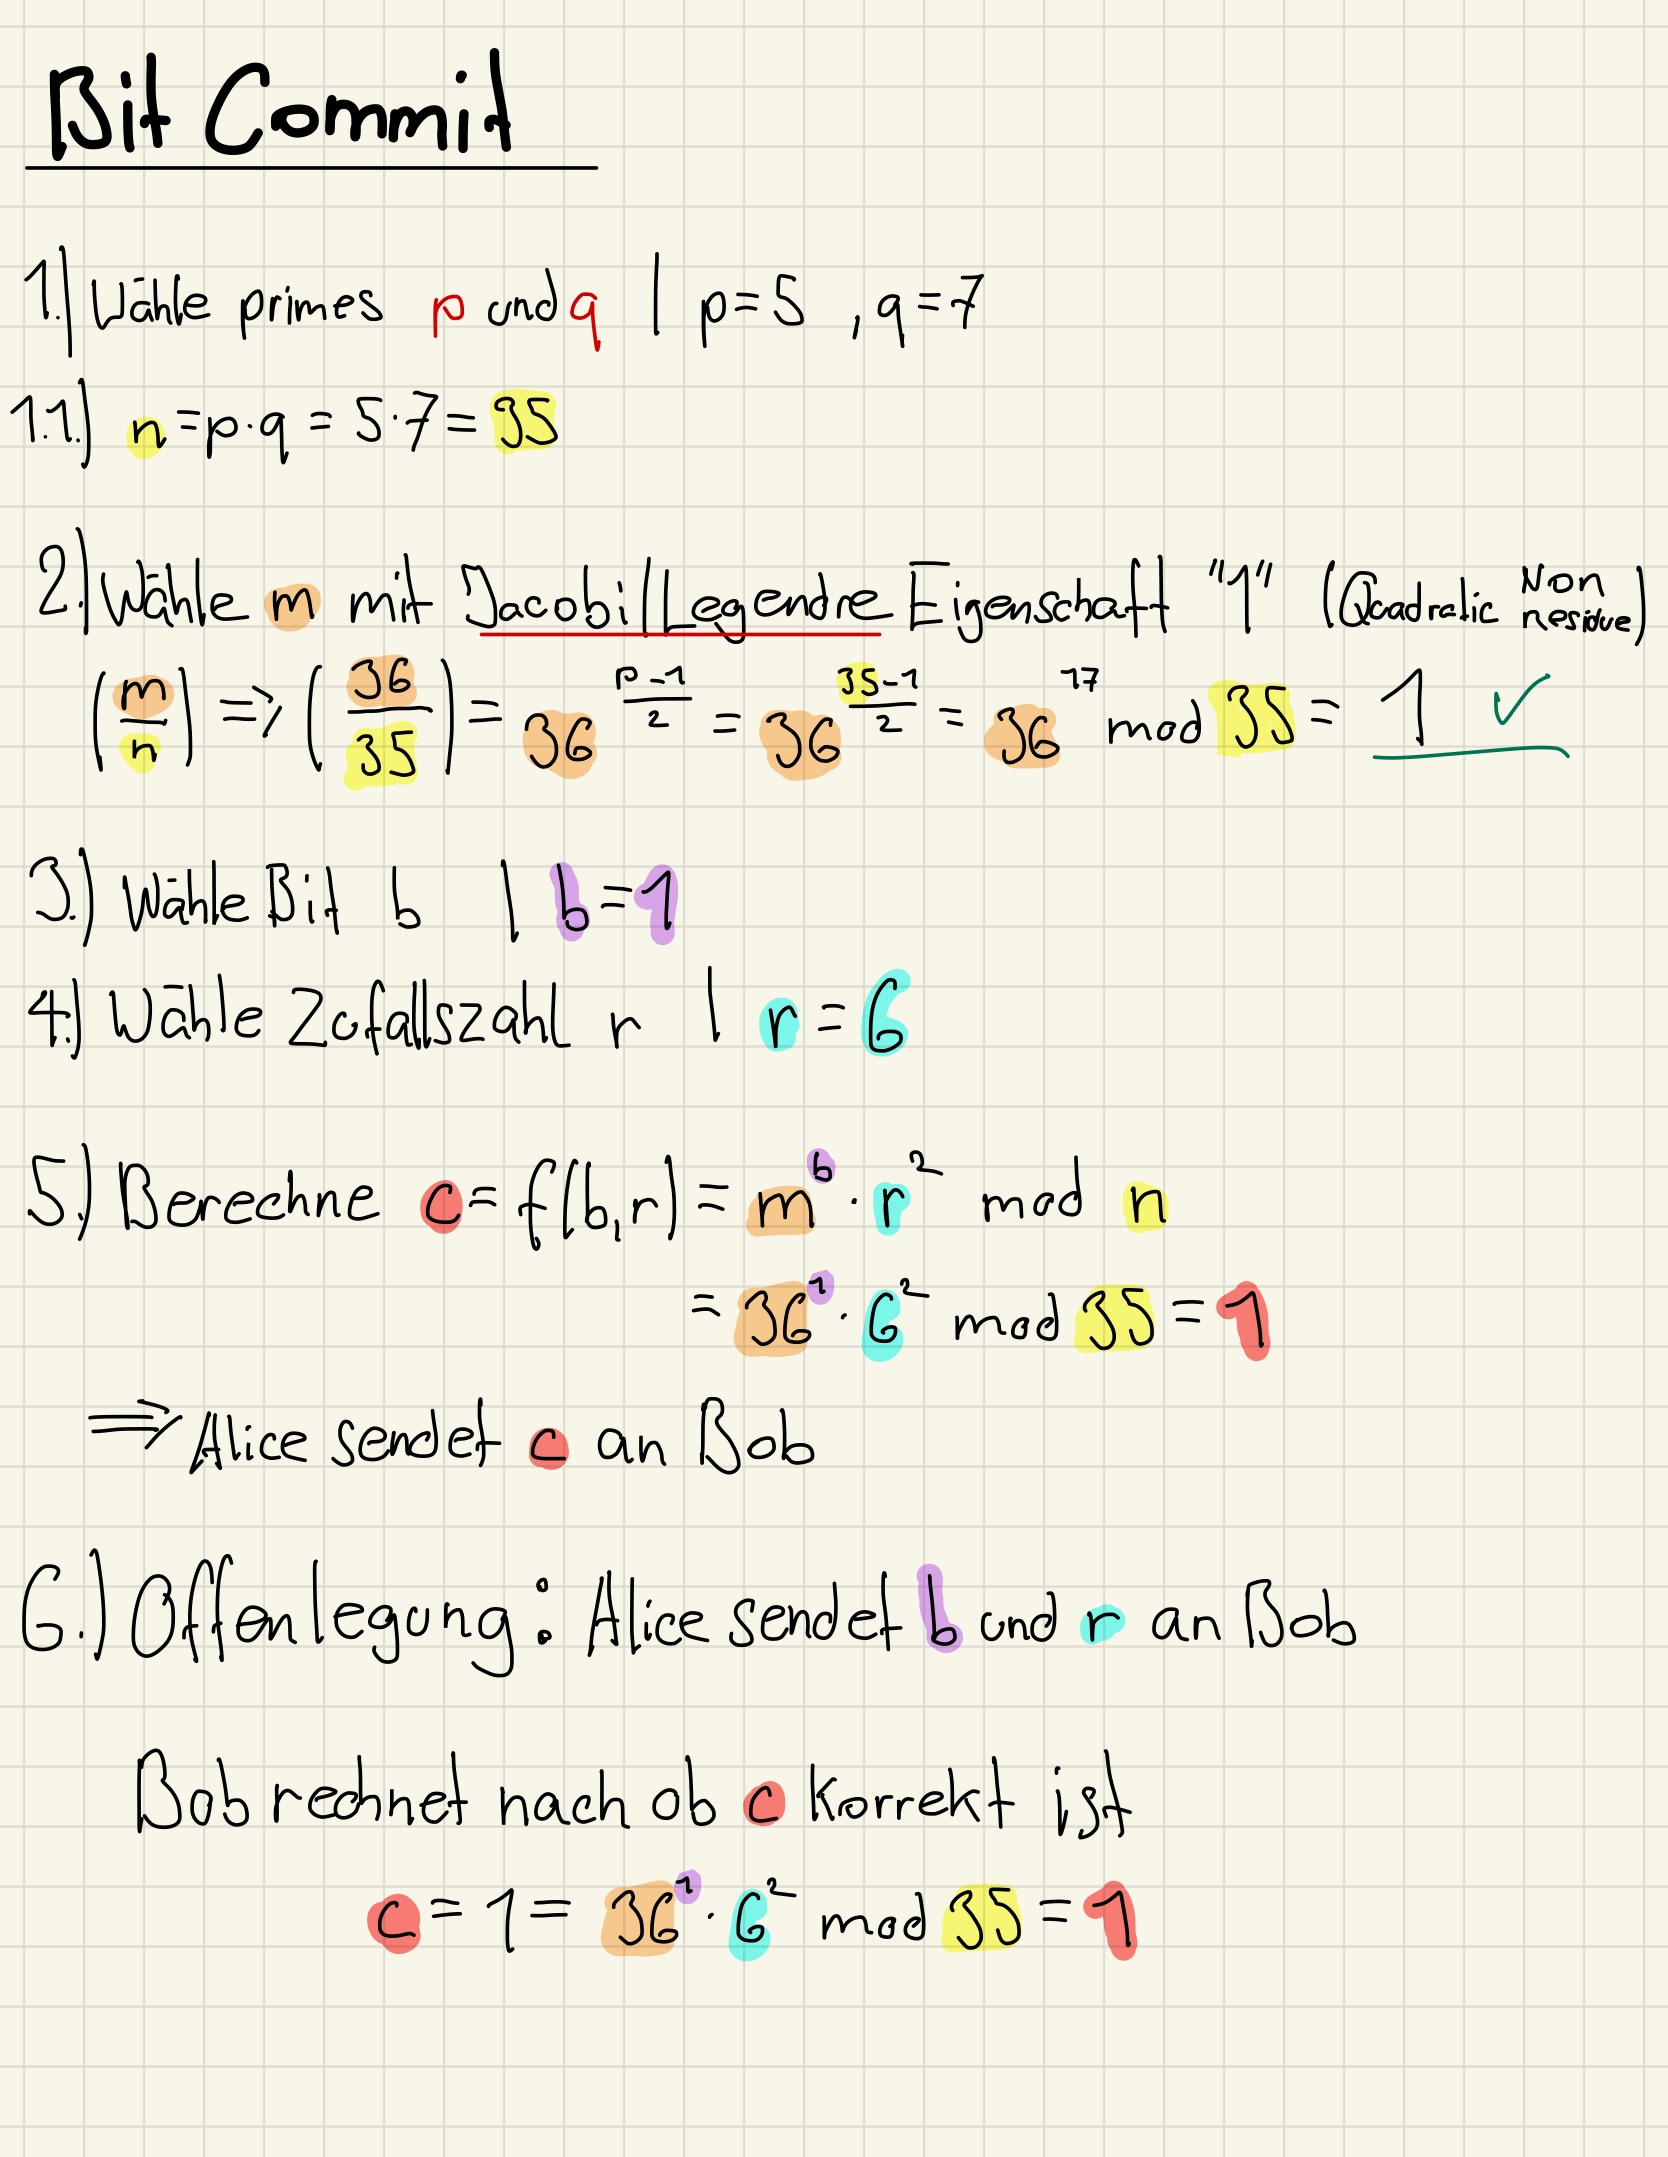
\includegraphics{img/bitcom.jpg}
\end{center}
    

    \hypertarget{sw08---protokolle-ii}{%
\section{SW08 - Protokolle II}\label{sw08---protokolle-ii}}

    \hypertarget{aufgabe-1-dining-cryptographers}{%
\subsection{1:
Dining-Cryptographers}\label{aufgabe-1-dining-cryptographers}}

Ziehen Sie das Protokoll Dining-Cryptographers im Falle einer
Dreiergruppe einige Male durch, indem sie das Protokoll mit einem
Schiedsrichter überprüfen:

\hypertarget{solution}{%
\subsubsection{Solution}\label{solution}}

David, Pascal, Stefan:

\textbf{Geheimes Bit erzeugen}

\(b_{DP}\) = 1, \(b_{DS}\) = 1

\(b_{PD}\) = 1, \(b_{PS}\) = 0

\(b_{SD}\) = 1, \(b_{SP}\) = 0

\textbf{XOR der jeweiligen Geheimen Bits berechnen}

David: \(b_{DP}\) + \(b_{DS}\) mod 2 = 1 + 1 mod 2 = 0

Pascal: \(b_{PD}\) + \(b_{PS}\) mod 2 = 1 + 0 mod 2 = 1

Stefan: \(b_{SP}\) + \(b_{SD}\) mod 2 = 0 + 1 mod 2 = 1

\textbf{Wenn der Kryptologe nicht bezahlen will, wird das XOR-Resultat
bekannt gegeben, möchte er bezahlen wird das Gegenteil vom XOR-Resultat
ausgegeben}

David hat ``0''. David bezahlt nicht und meldet deshalb ``0''\\
Pascal hat ``1'', Pascal bezahlt und meldet deshalb das Gegenteil, also
``0''\\
Stefan hat ``1''. Stefan bezahlt nicht und meldet deshalb ``1''

\textbf{Alle Ergebnisse nochmals XORen}

David + Pascal + Stefan mod 2 = 0 + 0 + 1 = 1 (Das bit ist 1, also hat 1
(gütiger) Kryptologe bezahlt.

\newpage

    \hypertarget{aufgabe-3-mixe}{%
\subsection{3: MIXe}\label{aufgabe-3-mixe}}

Beispiel MIXE

\hypertarget{solution}{%
\subsubsection{Solution}\label{solution}}

\begin{center}
	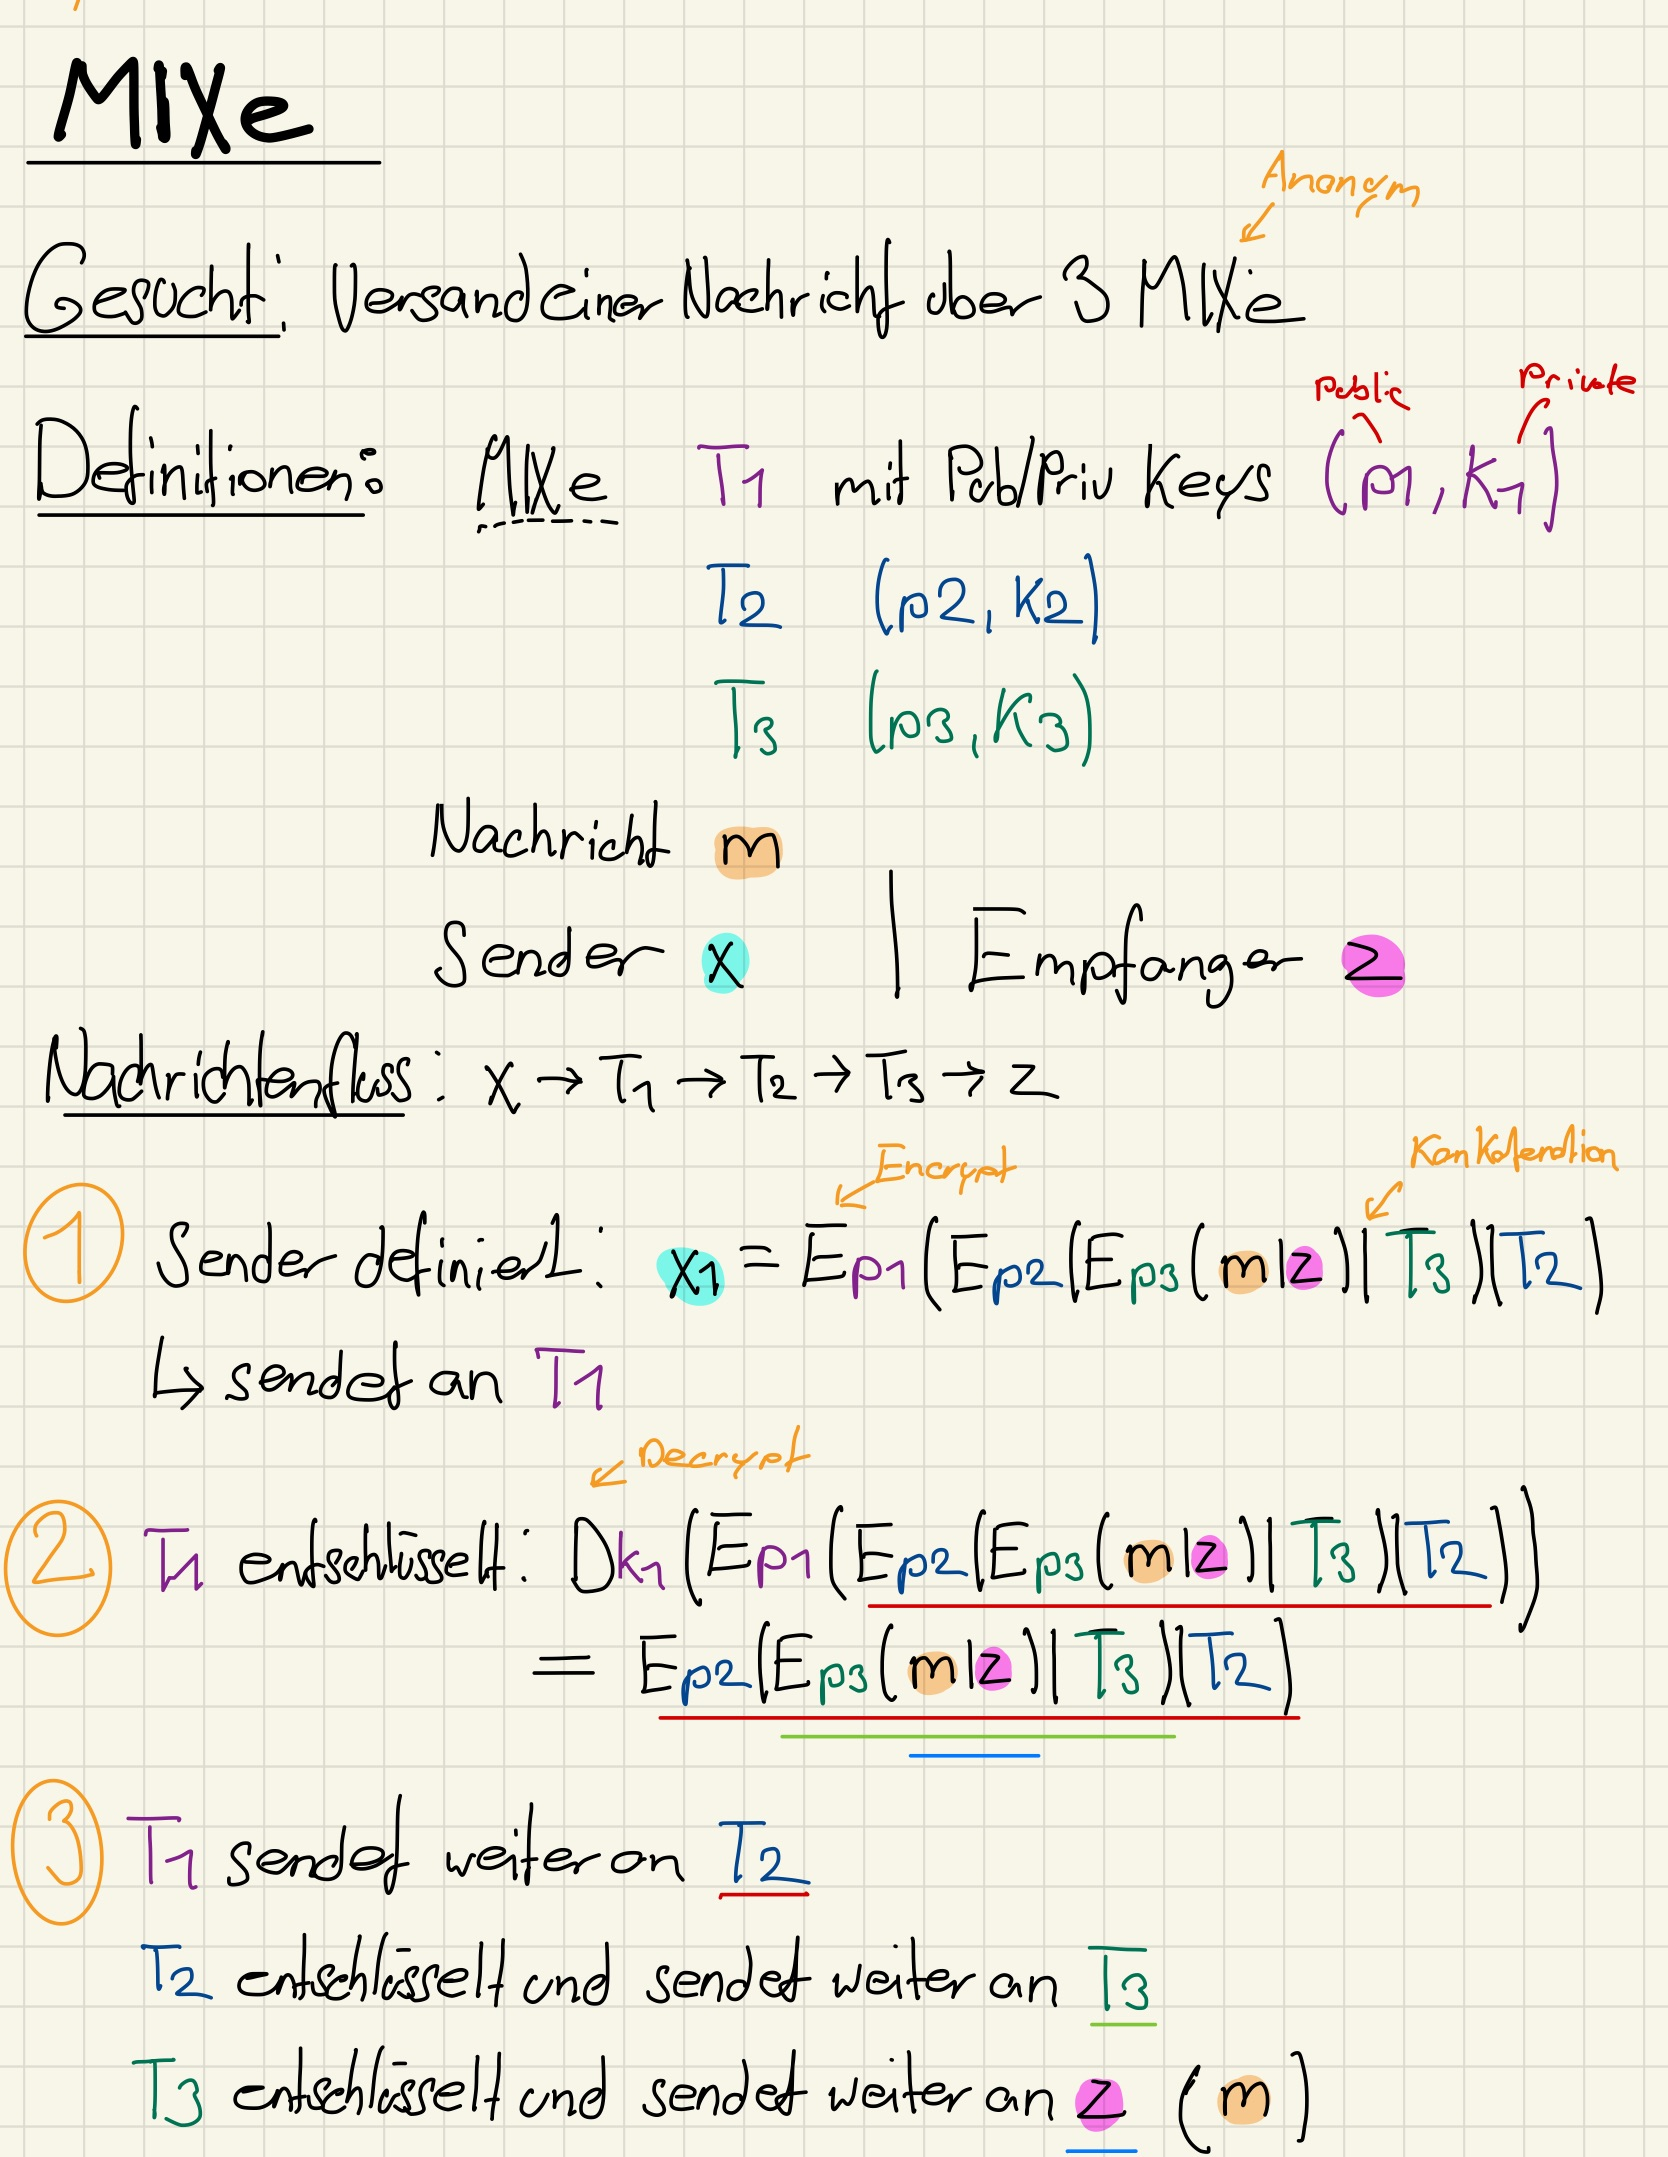
\includegraphics{img/mixe.jpg}
\end{center}

\newpage

    \hypertarget{aufgabe-5-secret-splitting-geteiltes-geheimnis}{%
\subsection{5: Secret Splitting / Geteiltes
Geheimnis}\label{aufgabe-5-secret-splitting-geteiltes-geheimnis}}

Verteilen Sie das Geheimnis 01011001 auf drei Leute! Protokollieren Sie
das Vorgehen und zeigen Sie, wie man das Geheimnis rekonstruiert.

\hypertarget{solution}{%
\subsubsection{Solution}\label{solution}}

\(M = 01011001\)

Alice: \(11001100 = A\)

Bob: \(10101010 = B\)

Cyril: \(A \oplus B \oplus M = 00111111 = C\)

\(M = A \oplus B \oplus C = 01011001\)

    \hypertarget{aufgabe-6-23-schwellenwertproblem---optional}{%
\subsection{6: (2,3)-Schwellenwertproblem -
(Optional)}\label{aufgabe-6-23-schwellenwertproblem---optional}}

Das Geheimnis \(M\) wird mit den drei Zufallszahlen \(R_1, R_2, R_3\) in
drei Teilgeheimnisse aufgeteilt. Das Teilgeheimnis
\(M_1=(M_{11},M_{12},M_{13})=(R_1 \oplus M, R_2,R_3)\) ist gegeben.

\begin{enumerate}
\def\labelenumi{\arabic{enumi}.}
\tightlist
\item
  Definieren Sie \(M_2\) und \(M_3\).\\
\item
  Rekonstruieren Sie \textbf{M} nur mit zwei Teilgeheimnissen
\end{enumerate}

\hypertarget{solution}{%
\subsubsection{Solution}\label{solution}}

\emph{Ist ähnlich wie die Aufgabe 5.}

Wir definieren z.B.
\(M_2=(M_{21},M_{22},M_{23})=(R_2 \oplus M, R_3,R_1)\)\\
Im Endefekkt haben wir etwas wie \(M_{11} = R_1 \oplus M\) und ebenfalls
\(M_{23} = R_1 \oplus M\)\\
Wir machen \(M_{11} \oplus M_{23}\), erhalten  \(R_{1} \oplus M \oplus R_{1}\) und so löst sich \(R_1\) auf und wir
haben sofort wieder \(M\).

    \hypertarget{aufgabe-8-threshold-verfahren-optional-2}{%
\subsection{8: Threshold-Verfahren (Optional
2)}\label{aufgabe-8-threshold-verfahren-optional-2}}

Alice teilt ein Geheimnis \(S\) mit einem Polynom des 2. Grades mit. Die
Zahl \(S\) ist die y-Achsenabschnitt (0, S), die das Geheimnis
darstellt. Als Teilgeheimnisse sind drei verschiedene Punkte
\((3, 2), (4, 1), (5, 2)\) bekannt. Wie rekonstruieren Sie das
Geheimnis?

\hypertarget{solution}{%
\subsubsection{Solution}\label{solution}}

Allgemeines Polynom zweiten Grades:
\[f(x) = a_2\cdot x^2 + a_1\cdot x^1 + a_0\cdot 1\]

\[ 2 = a_2\cdot 3^2 + a_1\cdot 3^1 + a_0\cdot 1\]
\[ 1 = a_2\cdot 4^2 + a_1\cdot 4^1 + a_0\cdot 1\]
\[ 2 = a_2\cdot 5^2 + a_1\cdot 5^1 + a_0\cdot 1\]

\[
\begin{bmatrix}
2\\
1\\
2\\
\end{bmatrix}
=
\begin{bmatrix}
9 & 3 & 1\\
16 & 4 & 1\\
25 & 5 & 1\\
\end{bmatrix}
\cdot
\begin{bmatrix}
a_2\\
a_1\\
a_0\\
\end{bmatrix}
\]

\emph{Dann hier etwas Linalg Python Magic, was an der MEP nicht möglich
ist :)}

\[
\begin{bmatrix}
a_2\\
a_1\\
a_0\\
\end{bmatrix}
=
\begin{bmatrix}
1\\
-8\\
17\\
\end{bmatrix}
\]

Und da \(S = a_0\) haben wir damit die Lösung \(S = 17\).

    

    \hypertarget{sw09---zertifikate-und-public-key-systeme}{%
\section{SW09 - Zertifikate und
Public-Key-Systeme}\label{sw09---zertifikate-und-public-key-systeme}}

    \hypertarget{aufgabe-1-zertifikate}{%
\subsection{Aufgabe 1: Zertifikate}\label{aufgabe-1-zertifikate}}

Erstellen Sie ein kurzes Protokoll zur Zertifikaterstellung und
Zertifikatüberprüfung.

\hypertarget{solution}{%
\subsubsection{Solution}\label{solution}}

\begin{enumerate}
\def\labelenumi{\arabic{enumi}.}
\tightlist
\item
  Hierzu erzeugt der Kunde im ersten Schritt auf seiner eigenen privaten
  Hardware ein Schlüsselpaar (einen privaten Schlüssel und einen
  öffentlichen).
\item
  Der Kunde erzeugt eine CSR-Datei, welche ein elektronisches Formular
  ist. Es enthält neben den Antragsdaten auch seinen öffentlichen
  Schlüssel.
\item
  Im dritten Schritt sendet der Kunde die CSR an die CA.
\item
  Die CA prüft den Antrag (also die CSR-Datei mit den Formularangaben
  und dem enthaltenden öffentlichen Zertifikat). Bei positiver Prüfung
  sendet die CA dem Käufer ein neues öffentliches Zertifikat zurück (als
  doppelt signierter öffentlicher Schlüssel).
\end{enumerate}

Für die Zertifikatsprüfung kann nun der öffentliche Schlüssel der von
Alice bereitgestellt wird von einer Drittperson mit dem öffentlichen
Schlüssel der signing CA vergleichen.

    \hypertarget{aufgabe-2-zertifikatshierarchie}{%
\subsection{Aufgabe 2:
Zertifikatshierarchie}\label{aufgabe-2-zertifikatshierarchie}}

\begin{enumerate}
\def\labelenumi{\arabic{enumi}.}
\tightlist
\item
  Welche Vorteile hat eine Zertifikatshierarchie für eine Firma und für
  die einzelne Benutzerin?
\item
  Welche Nachteile hat eine Zertifikatshierarchie für eine Firma und für
  den einzelnen Benutzer?
\end{enumerate}

\hypertarget{solution-quick}{%
\subsubsection{Solution Quick}\label{solution-quick}}

\begin{enumerate}
\def\labelenumi{\arabic{enumi}.}
\item
  Zertifikatsbasierte authentifizierungen vereinfachen das gesamte
  Authentifizierungsverfahren. Durch eine eigene CA hat man in der Firma
  volle Kontrolle über die Zertifikate und muss nicht über eine public
  CA gehen.
\item
  Das Problem sind vorallem die Trusts mit anderen Firmen/CA's. Hierfür
  muss immer jeweils das Root Zertifikat der anderen Firmen im
  Truststore eingespielt werden.
\end{enumerate}

    

    \hypertarget{sw10---homomorphe-verschluxfcsselung}{%
\section{SW10 - Homomorphe
Verschlüsselung}\label{sw10---homomorphe-verschluxfcsselung}}

    \hypertarget{aufgabe-1-homomorphe-verschluxfcsselung}{%
\subsection{Aufgabe 1: Homomorphe
Verschlüsselung}\label{aufgabe-1-homomorphe-verschluxfcsselung}}

\begin{enumerate}
\def\labelenumi{\arabic{enumi}.}
\tightlist
\item
  Welches der drei Verschlüsselungsverfahren (RSA, EL-GAMAL, Paillier)
  ist eher geeignet für die Verwendung in homomorpher Verschlüsselung
  eingesetzt werden? Begründen bitte Ihre Antwort?
\item
  Geben Sie ein Beispiel, in welchem Bereich das Paillier-Verfahren
  eingesetzt werden könnte? Begründen Sie Ihre Antwort?
\end{enumerate}

\hypertarget{solution}{%
\subsubsection{Solution}\label{solution}}

\begin{center}
	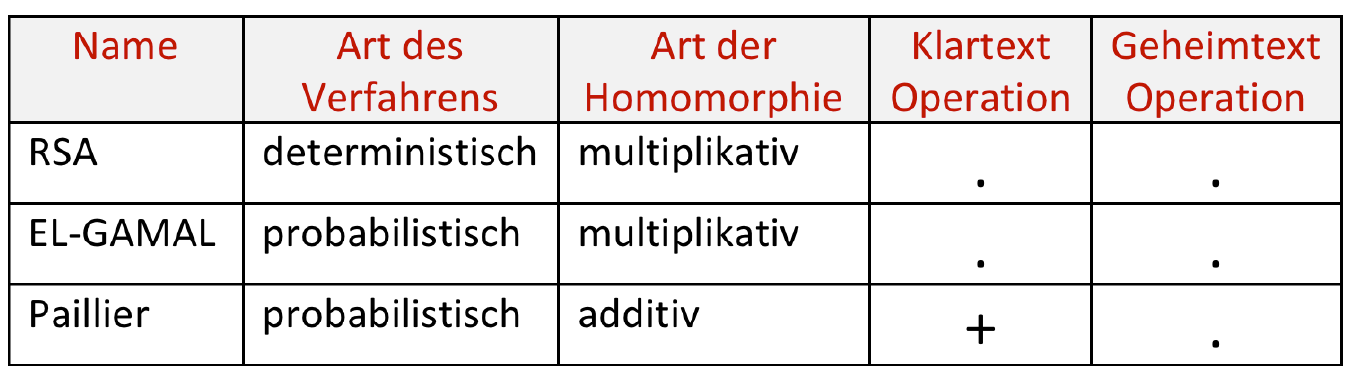
\includegraphics[scale=0.6]{img/algoverview.png}
\end{center}

\begin{enumerate}
\def\labelenumi{\arabic{enumi}.}
\item
  RSA ist semantisch nicht korrekt, da durch Polluting (rauschen) das
  Ver+Entschlüsseln nicht immer dasselbe ergeben. Konkret wenn das
  Rechenergebnis grösser als der Modulus ist, wird das Resultat
  ``abgeschnitten''. Elgamal und Paillier sind besser geeignet da sie
  semantisch sind. Jedoch ist Elgamal nur für die Multiplikation und
  Paillier nur für die Addition geeignet (kommt halt auf den
  Einsatzzweck an). Paillier ist ausserdem sehr komplex und
  rechenintensiv.
\item
  Paillier könnte z.B. für E-Voting genutzt werden. So könnte man alle
  abgegebenen Stimmen zählen (addieren) ohne zu sehen wer konkret wen
  gewählt hat
\end{enumerate}

    \hypertarget{aufgabe-2-homomorphie-eigenschaft-von-el-gamal}{%
\subsection{Aufgabe 2: Homomorphie-Eigenschaft von
EL-GAMAL}\label{aufgabe-2-homomorphie-eigenschaft-von-el-gamal}}

Berechnen Sie bitte jeden Schritt im unteren Teil des Beispiels (s.
unten). Die Berechnung für den oberen Teil finden Sie auf den Folien
SW10

\begin{center}
	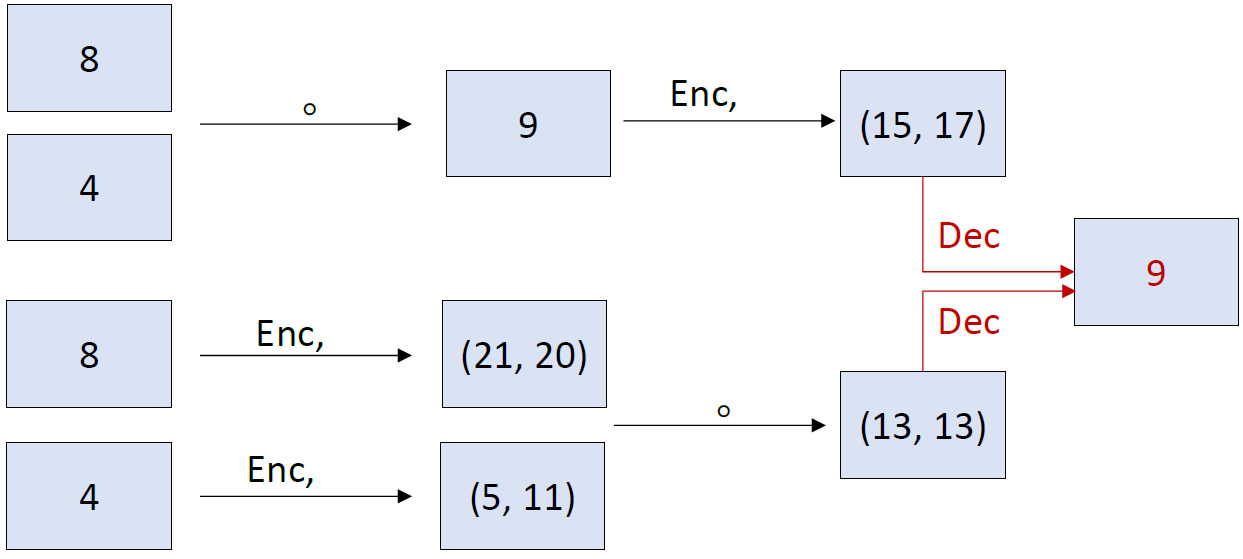
\includegraphics[scale=0.6]{img/elgamal.png}
\end{center}

\hypertarget{solution}{%
\subsubsection{Solution}\label{solution}}


\begin{center}
	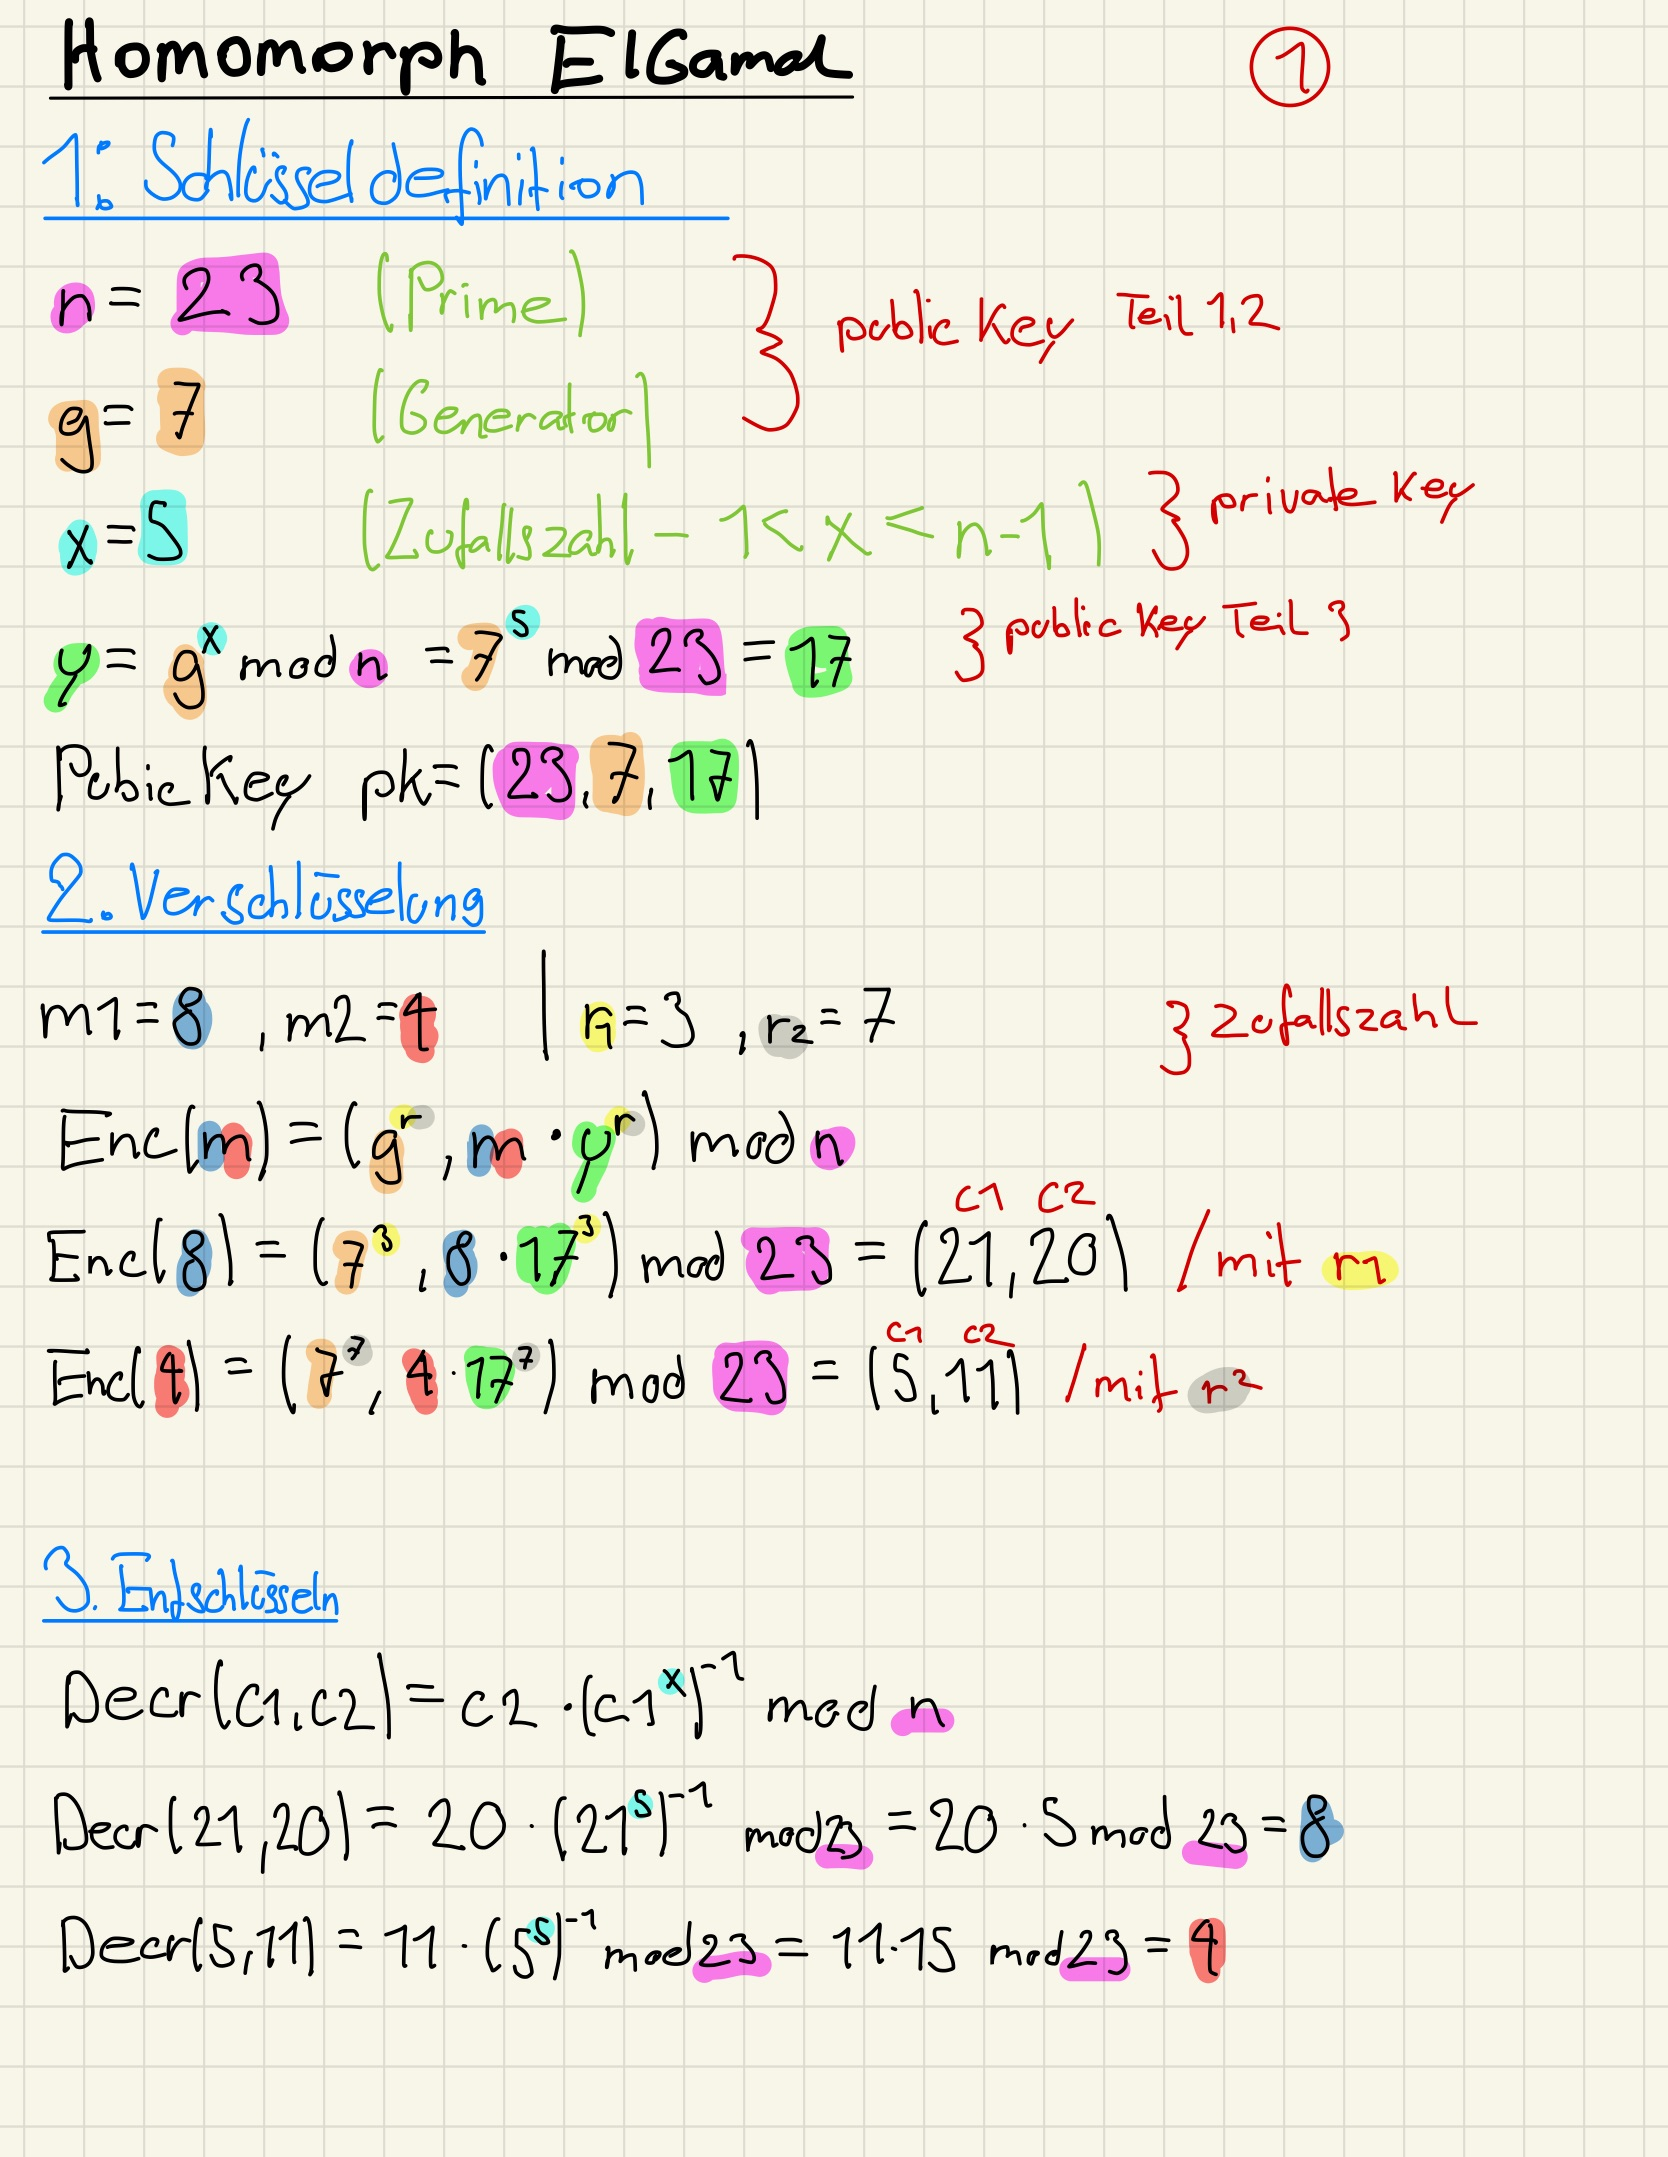
\includegraphics[scale=0.93]{img/helg1.jpg} \\
\end{center}

\break

\begin{center}
	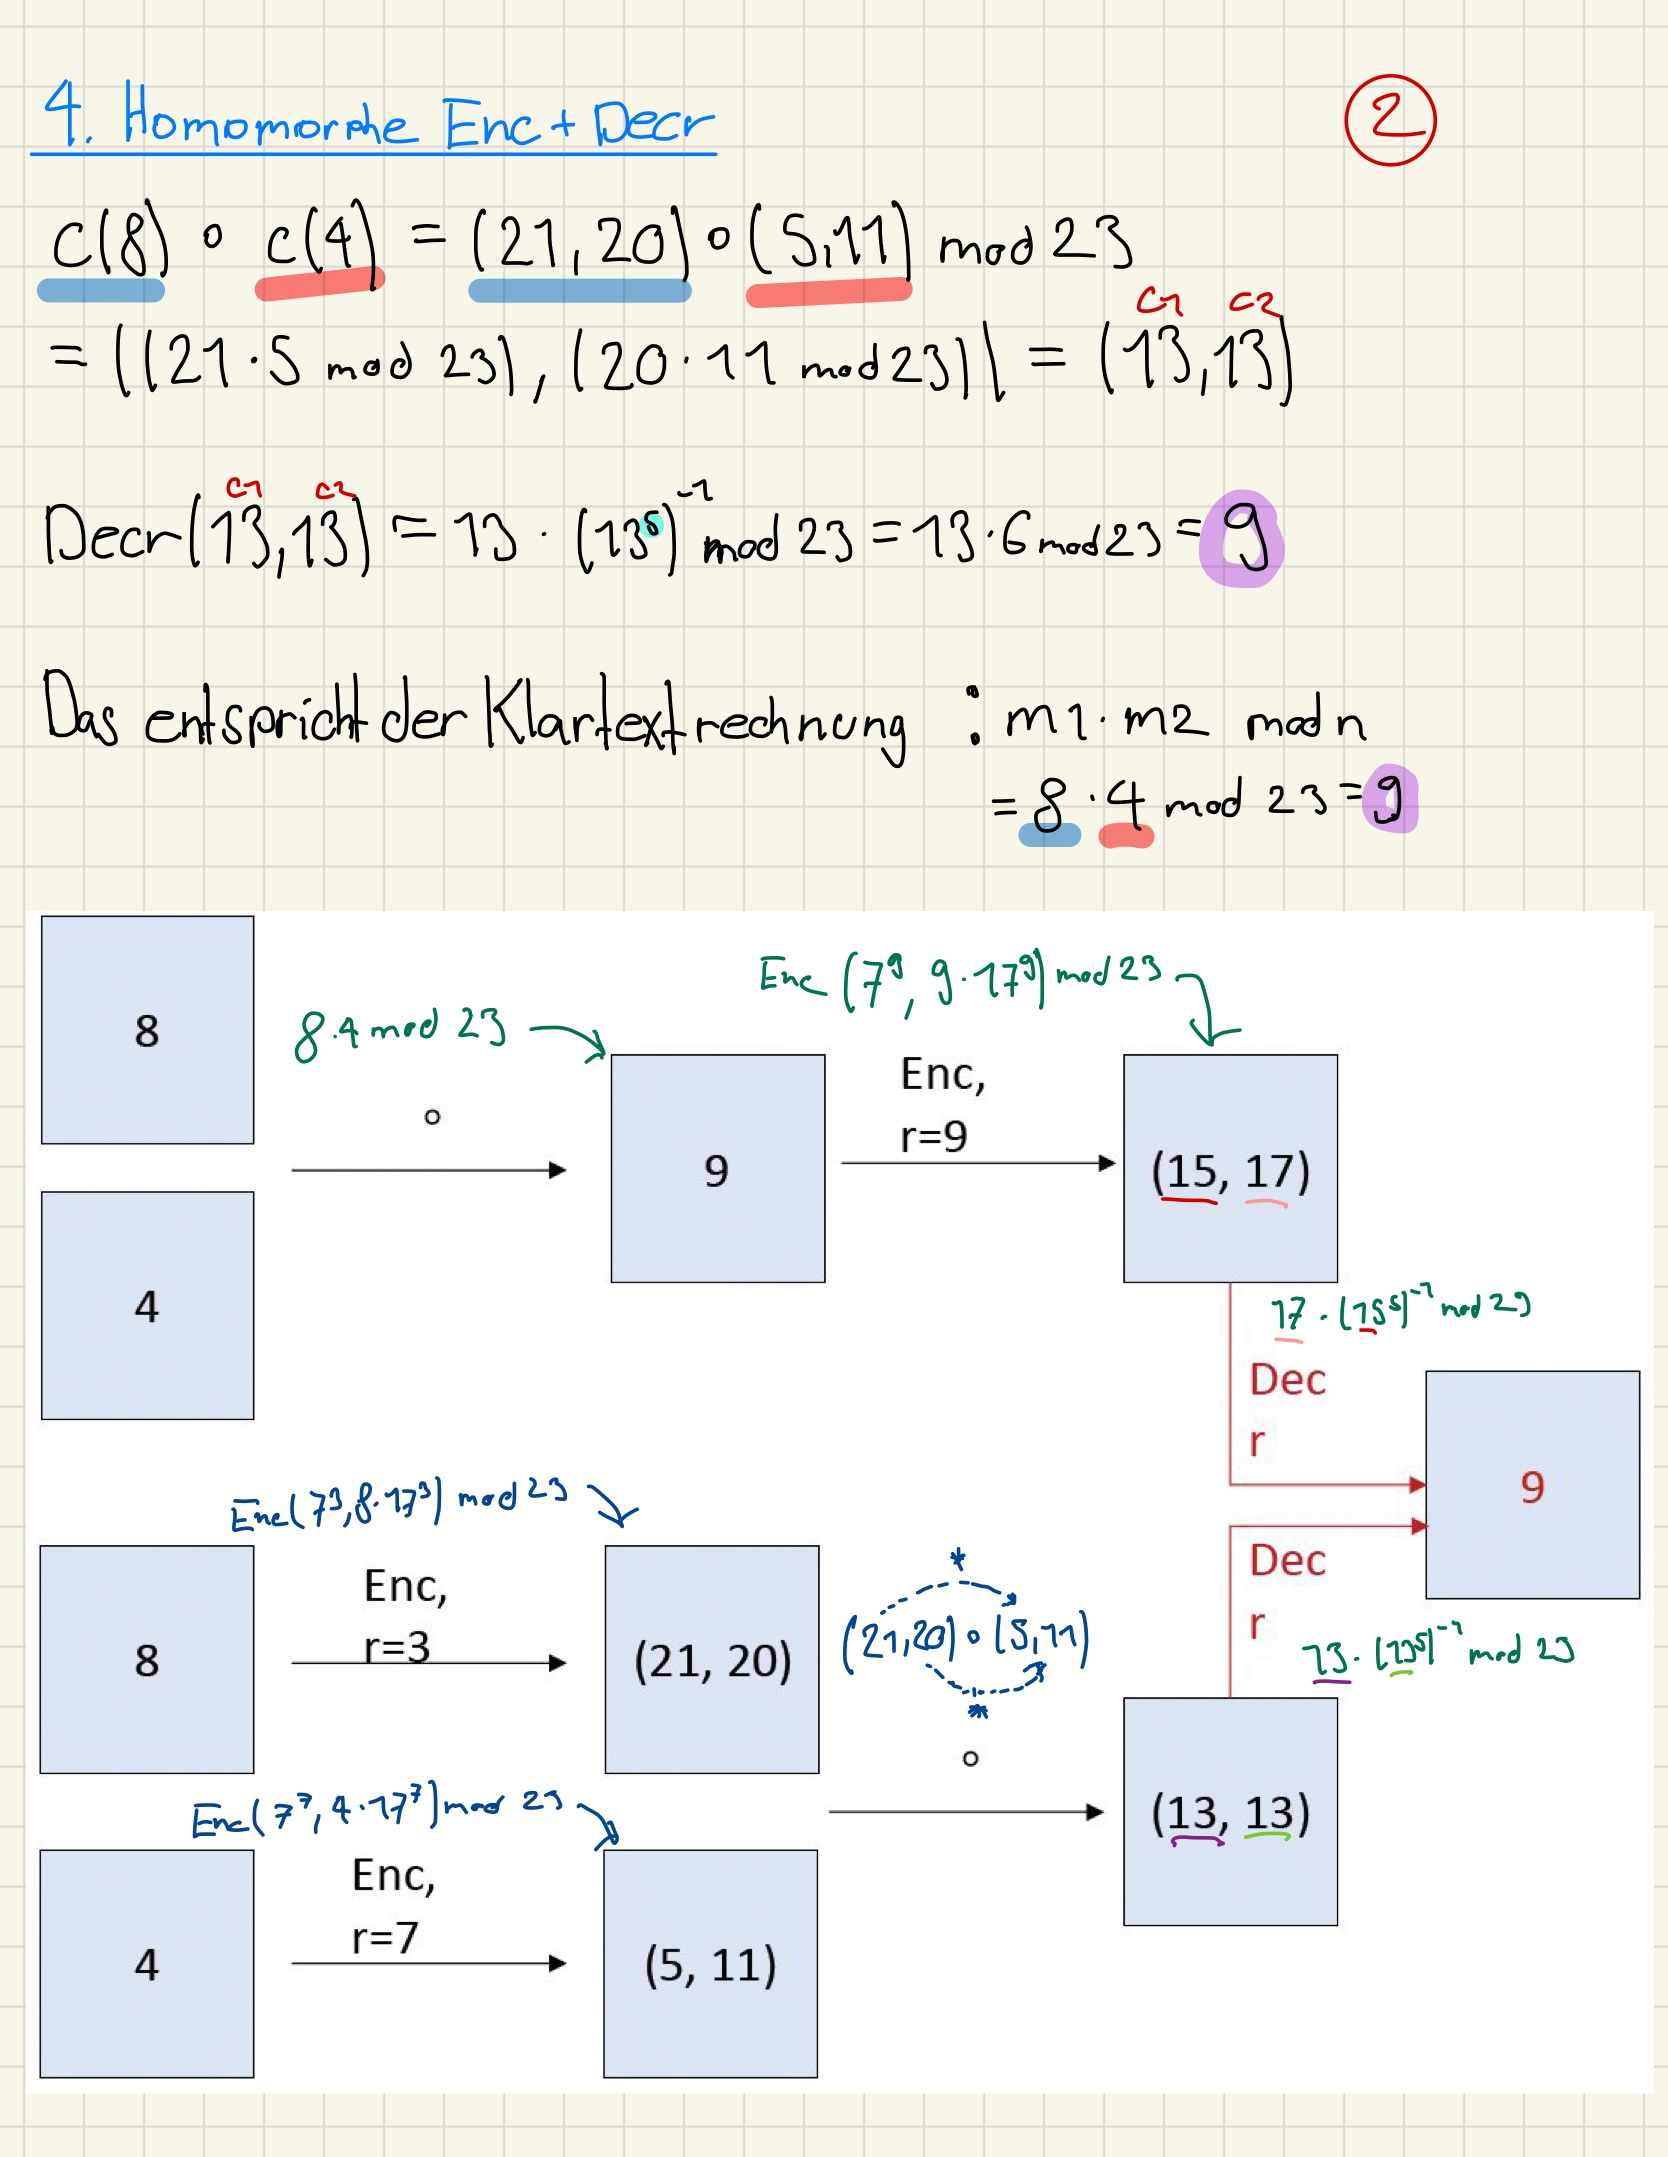
\includegraphics[scale=0.96]{img/helg2.jpg} \\
\end{center}


\newpage

    \hypertarget{aufgabe-3-paillier-verfahren}{%
\subsection{Aufgabe 3:
Paillier-Verfahren}\label{aufgabe-3-paillier-verfahren}}

Gegeben sind zwei Primzahlen \textbf{p}=3 und \textbf{q}=5. Sei
\textbf{g}=16 aus \(Z^{*}_{225}\) zufällig gewählt. \\
1. Berechnen Sie
jeweils den öffentlichen und privaten Schlüssel. \\
2. Verschlüssen Sie den
Klartext m=13. \\
3. Entschlüssen Sie den Ciphertext c=71.

\hypertarget{solution}{%
\subsubsection{Solution}\label{solution}}

\begin{center}
	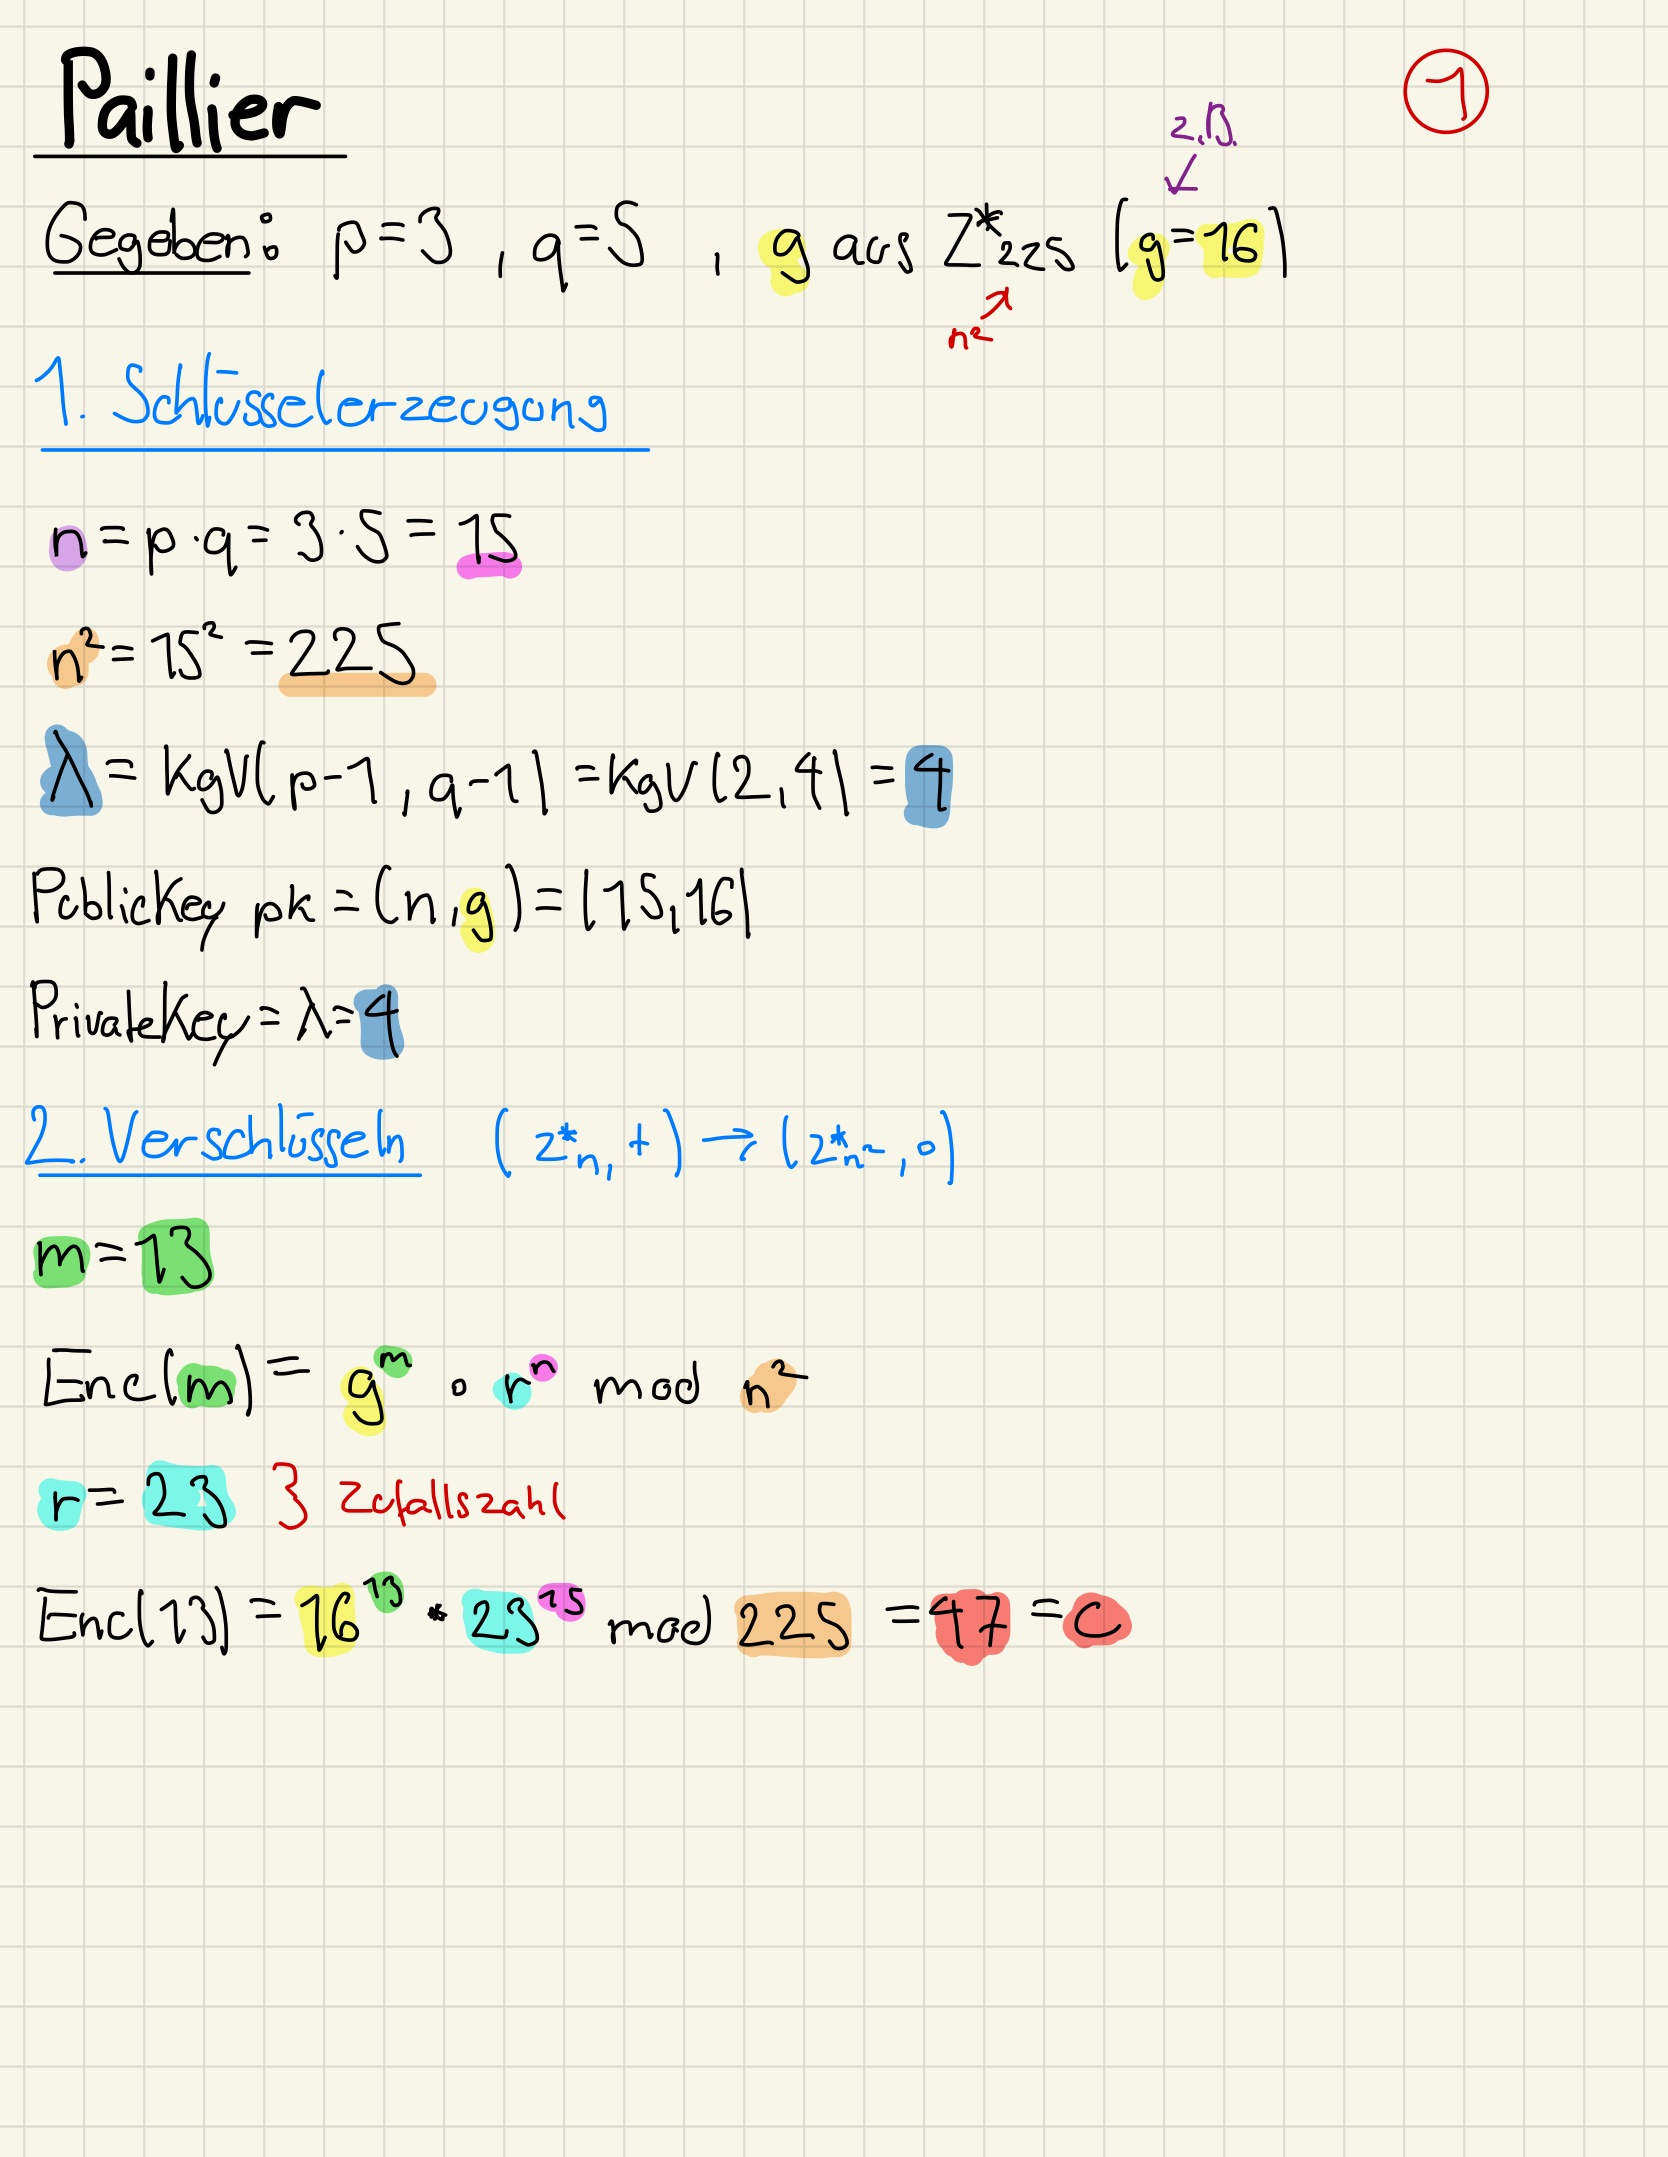
\includegraphics[scale=0.9]{img/pail1.jpg}\\
\end{center}

\break

\begin{center}
	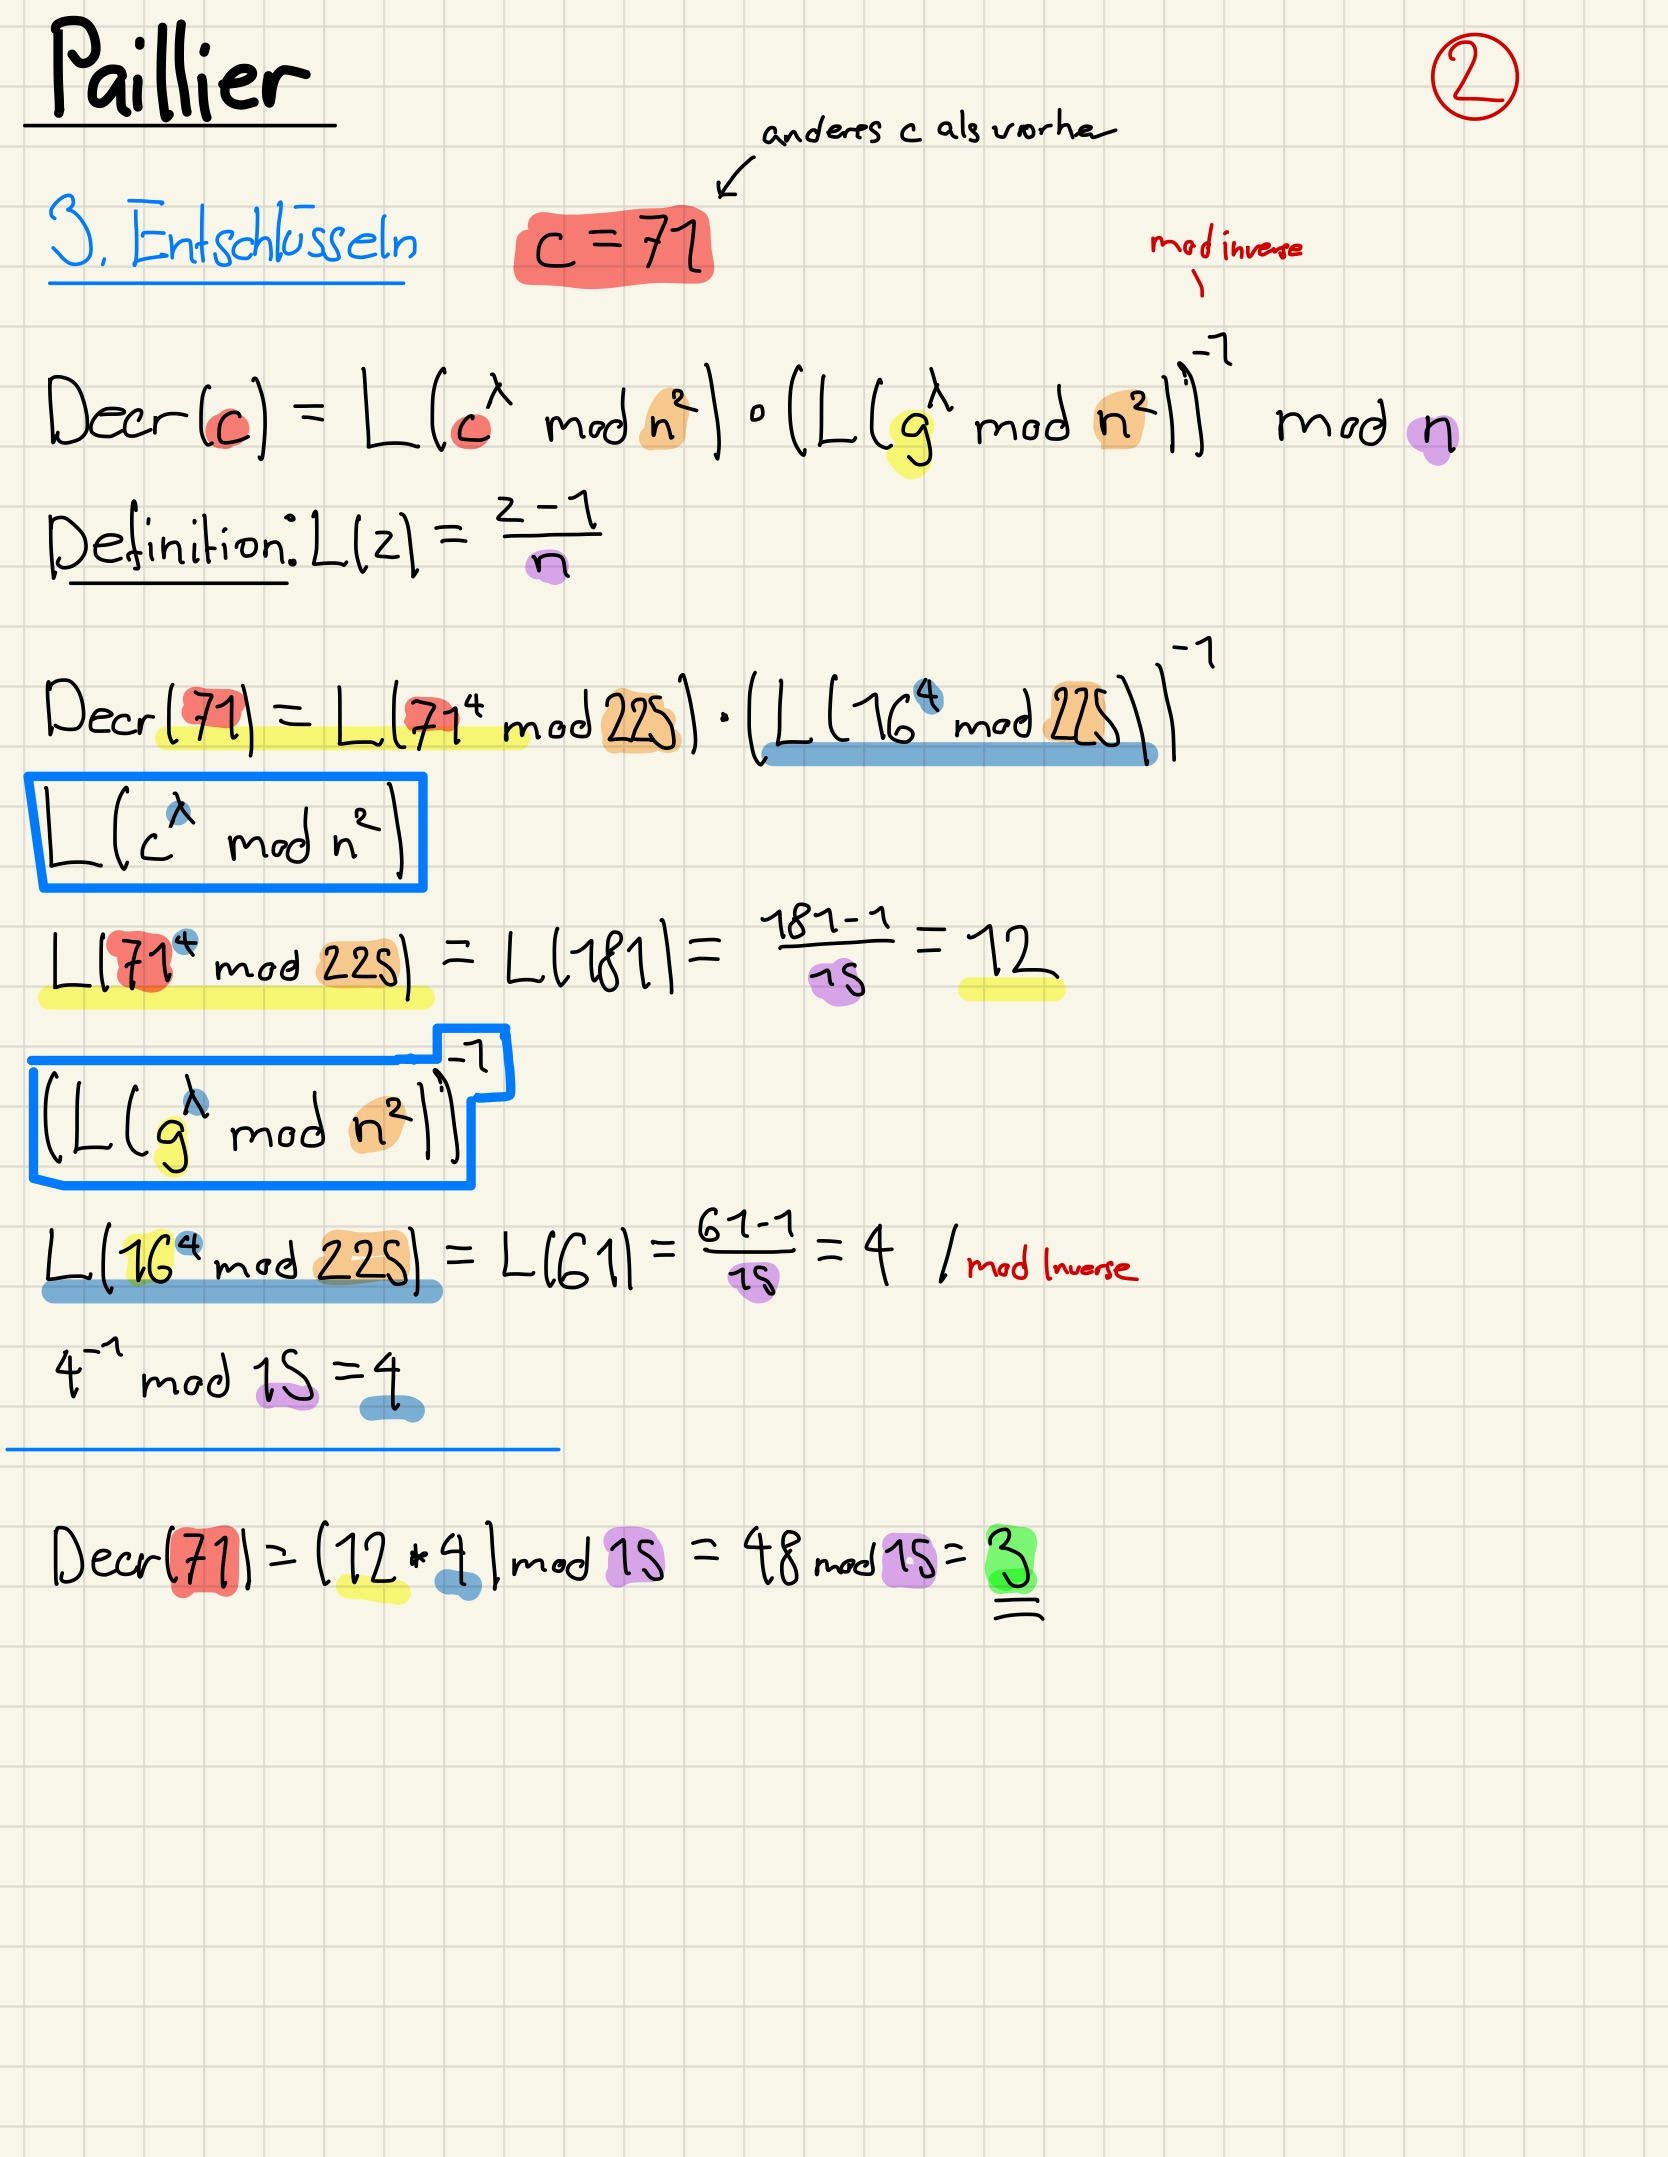
\includegraphics[scale=0.95]{img/pail2.jpg}\\
\end{center}

\newpage   

    \hypertarget{sw11---evoting}{%
\section{SW11 - eVoting}\label{sw11---evoting}}

    \hypertarget{aufgabe-2-wahlprotokoll-mit-symmetrischer-verschluxfcsselung}{%
\subsection{Aufgabe 2: Wahlprotokoll mit symmetrischer
Verschlüsselung}\label{aufgabe-2-wahlprotokoll-mit-symmetrischer-verschluxfcsselung}}

Wir betrachten zwei Wählerinnen Alice und Eve. Am Ende des symmetrischen
eVoting Protokolls mit blinder Signatur möchte Eve ermitteln, wie Alice
gewählt hat.\\
Kann Sie es? Begründen Sie Ihre Antwort.

\hypertarget{solution}{%
\subsubsection{Solution}\label{solution}}

\textbf{Nein}, Eve kann nicht ermitteln, was Alice gewählt hat. Das wäre
nur möglich, wenn Eve im Zählsystem oder als Administrator fungieren
würde. So hätte sie die Möglichkeit, die verschlüsselte Stimme von Alice
zu rekonstruieren oder aufgrund des von Alice ans Zählsystem übergebenen
Schlüssels K die zugehörige Stimme ausfindig zu machen.\\
Aber da Eve ebenfalls Wählerin ist und sie lediglich die am Ende vom
Zählsystem veröffentlichte Liste mit den verschlüsselten Stimmen (samt
Schlüssel) sehen kann, hat sie keine Möglichkeit, eine der Stimmen genau
Alice zuzuordnen, da sie nicht Alices Schlüssel K kennt.

    \hypertarget{aufgabe-3-additives-homomorphes-wahlprotokoll}{%
\subsection{Aufgabe 3: additives homomorphes
Wahlprotokoll}\label{aufgabe-3-additives-homomorphes-wahlprotokoll}}

``Verschlüssle alle Wahlergebnisse (\(ri\) und `Gewähltes' als \(m\))
und zähle sie mit dem Paillier Verfahren zusammen (homomorphe Addition).
Entschlüssle die Ergebnisse anschliessend und leite von der erhaltenen
Zahl das Ergebniss ab.''

Bedeutung: ``10=ja'' und ``1=nein''

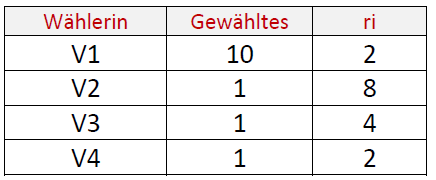
\includegraphics[scale=0.5]{img/votetable.png}

Die Verschlüsselung von der Aufgabe 3 (SW10):

p = 3\\
q = 5\\
n = p*q = 15\\
g = 16\\
\(\lambda\) = kgV((p-1) * (q-1)) = 4.

\hypertarget{solution}{%
\subsubsection{Solution}\label{solution}}

\begin{center}
	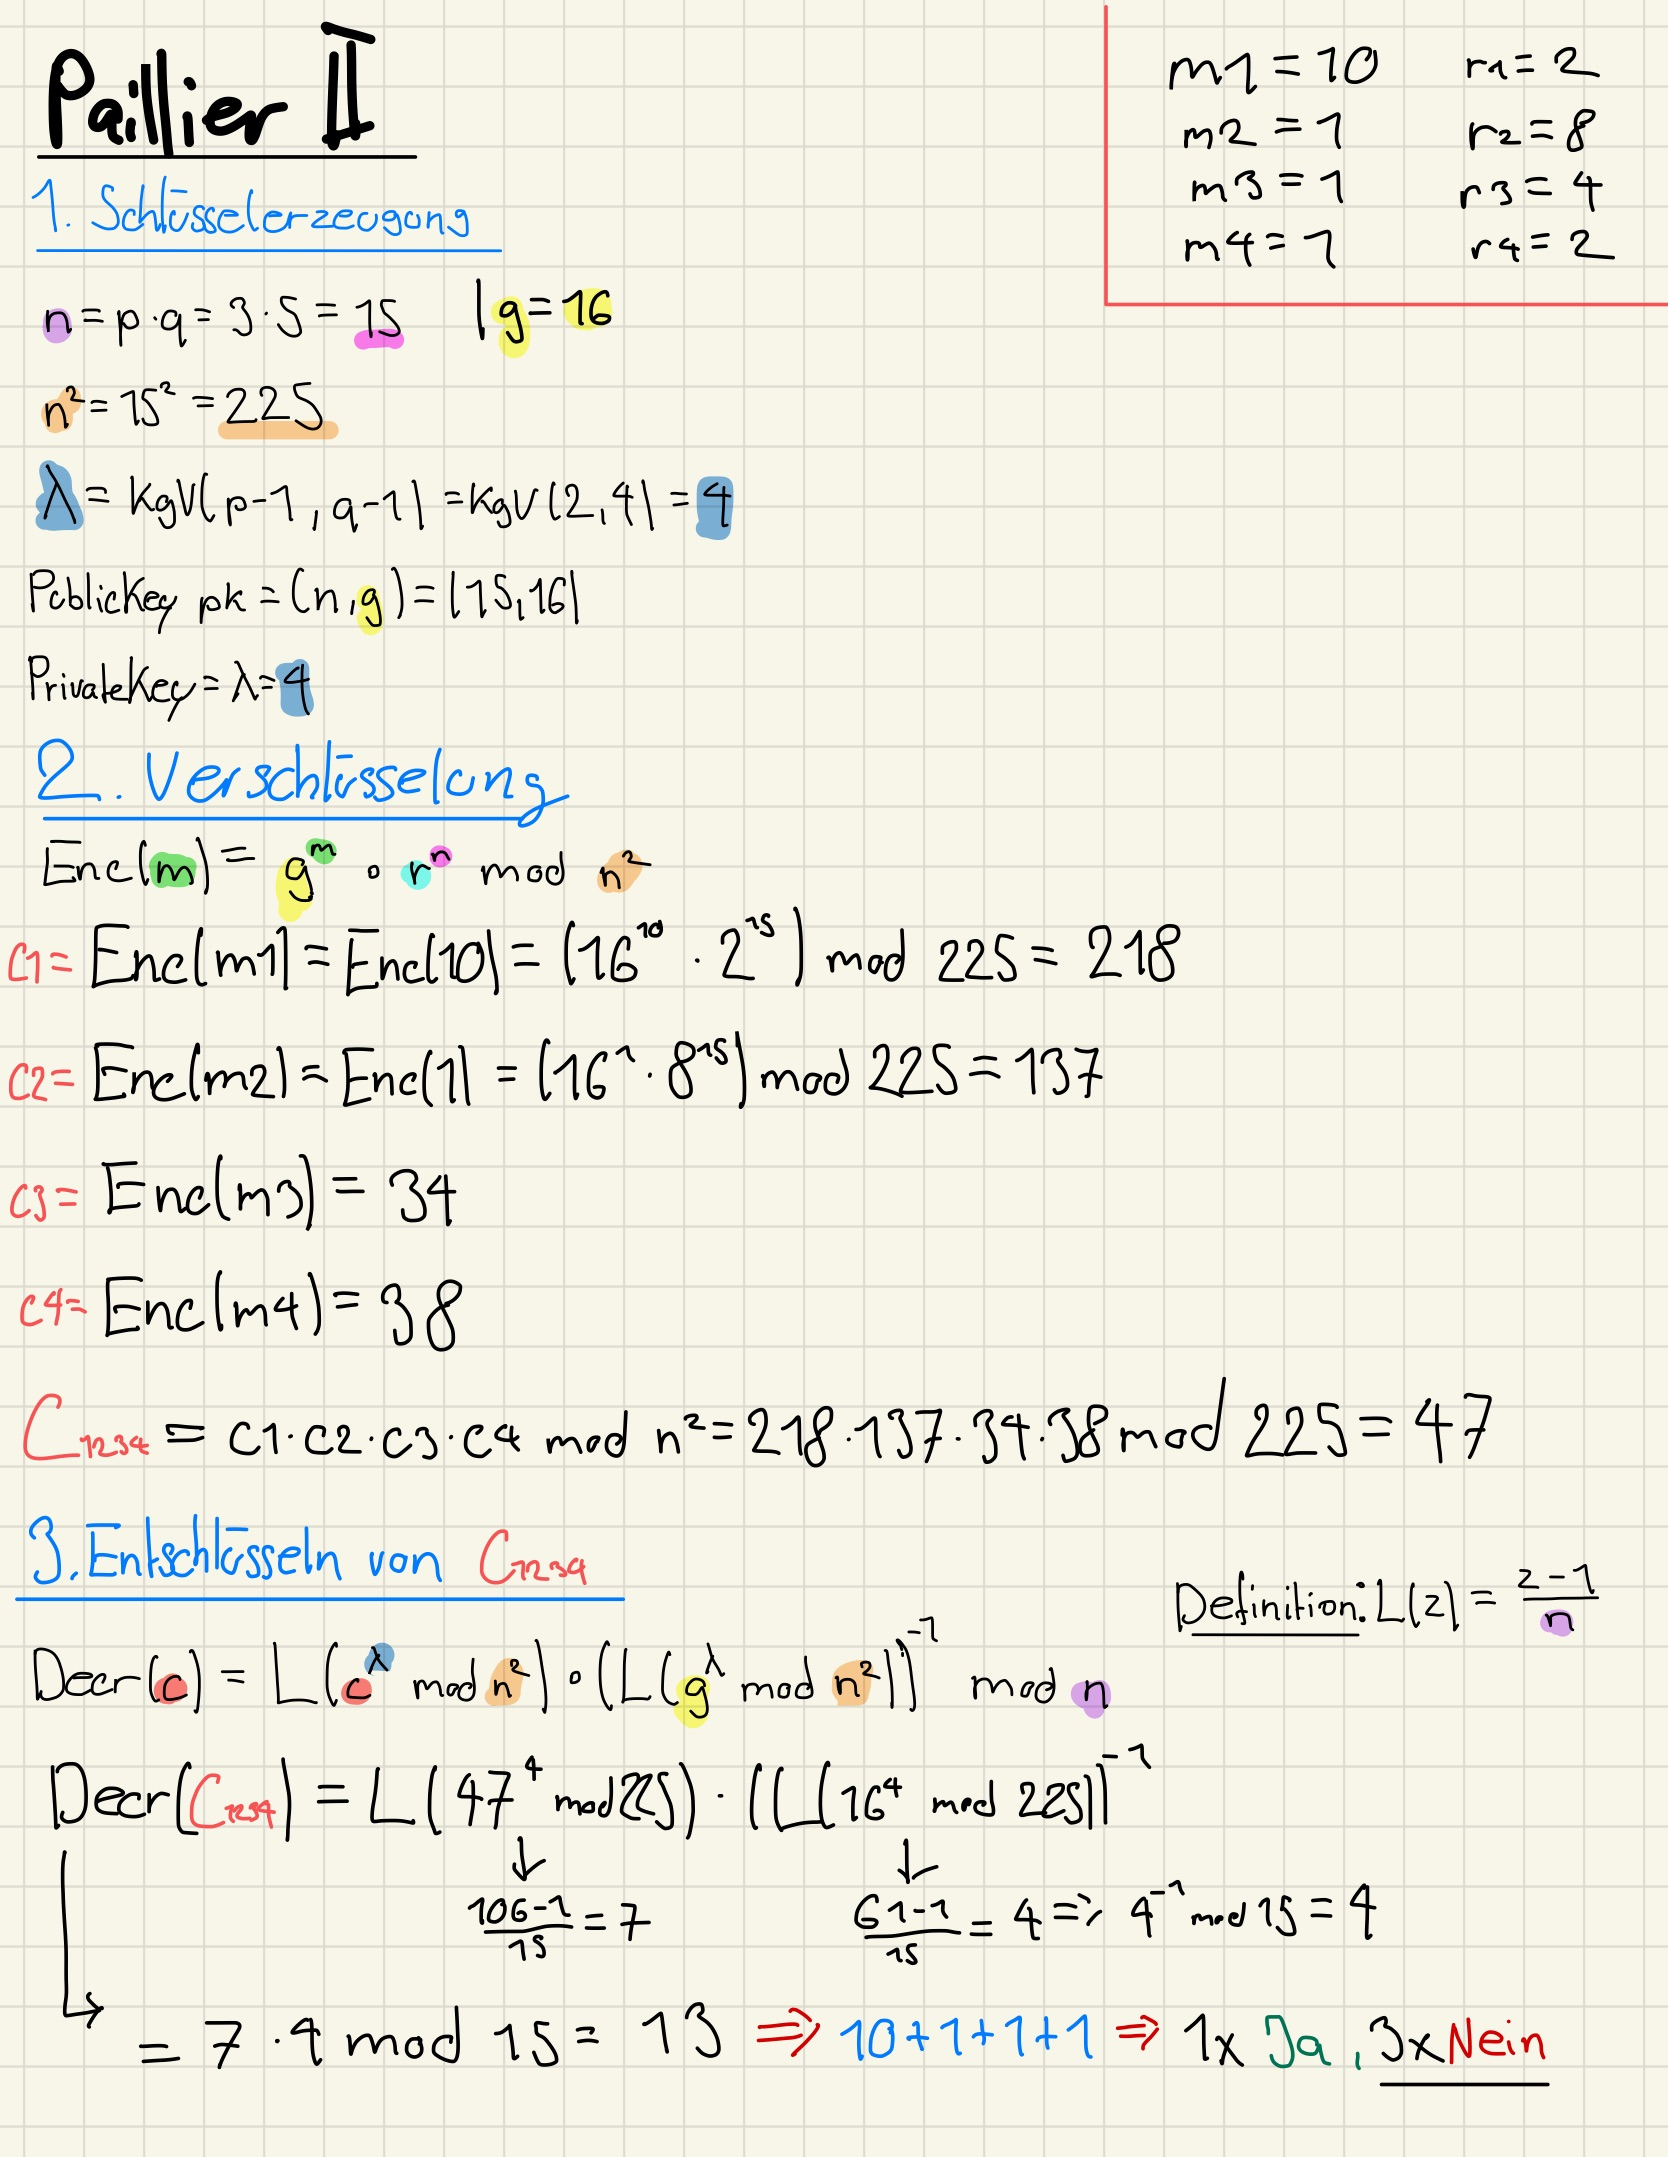
\includegraphics[scale=0.9]{img/pail2_sw11.jpg}
\end{center}
    

    \hypertarget{sw12---epayment}{%
\section{SW12 - ePayment}\label{sw12---epayment}}

    \hypertarget{aufgabe-2-random-serialnumber}{%
\subsection{Aufgabe 2: Random
Serialnumber}\label{aufgabe-2-random-serialnumber}}

Das Protokoll von E-Cash entwickelt von der Firma Digicash sieht eine
zufällig gewählte\\
Seriennummer \(S\) für jede eMünze vor. Sollte \(S\) zufällig gewählt
werden oder sollte \(S\) wie die Zahl \(X\) im
Wahlzettel für eVoting von einer bestimmten Struktur sein?

\hypertarget{solution}{%
\subsubsection{Solution}\label{solution}}

Die Seriennummer sollte nicht Random sein, da man sonst leicht einen
Betrugsversuch machen könnte ala:

\begin{itemize}
\item
  Mallory nimmt generiert eine zufällige Zahl \(C\) und verschlüsselt
  mit einem Public-Key (e,d): \(S=C^{e}\)
\item
  Mit \(C = S^{d}\) kann die Zahl korrekt entschlüsselt werden und
  man könnte meinen es sei eine richtige Seriennummer.
\end{itemize}

Ein Beispiel für eine gute Seriennummer Struktur wäre ein Hash von
relevanten Daten der Münze (Issuer, Betrag, Gültigskeitszeitraum)

    \hypertarget{aufgabe-4-serialnumber-bits}{%
\subsection{Aufgabe 4: Serialnumber
Bits}\label{aufgabe-4-serialnumber-bits}}

Wie viele Bit muss die zufällig generierte Seriennummer einer E-Münze
lang sein, damit die\\
Wahrscheinlichkeit für eine zufällige Übereinstimmung von zwei Nummern
kleiner ist als die\\
Wahrscheinlichkeit, bei zwei aufeinander folgenden Ziehungen im Lotto (6
aus 49) sechs Richtige zu
tippen? \\
Tipp: Berechnen Sie zuerst die Wahrscheinlichkeit, mit einer
zufällig erzeugten Seriennummer 
eine vorgegebene Zahl fester Länge zu treffen. Bestimmen Sie dann deren
Länge \textbf{n}.

\hypertarget{solution}{%
\subsubsection{Solution}\label{solution}}

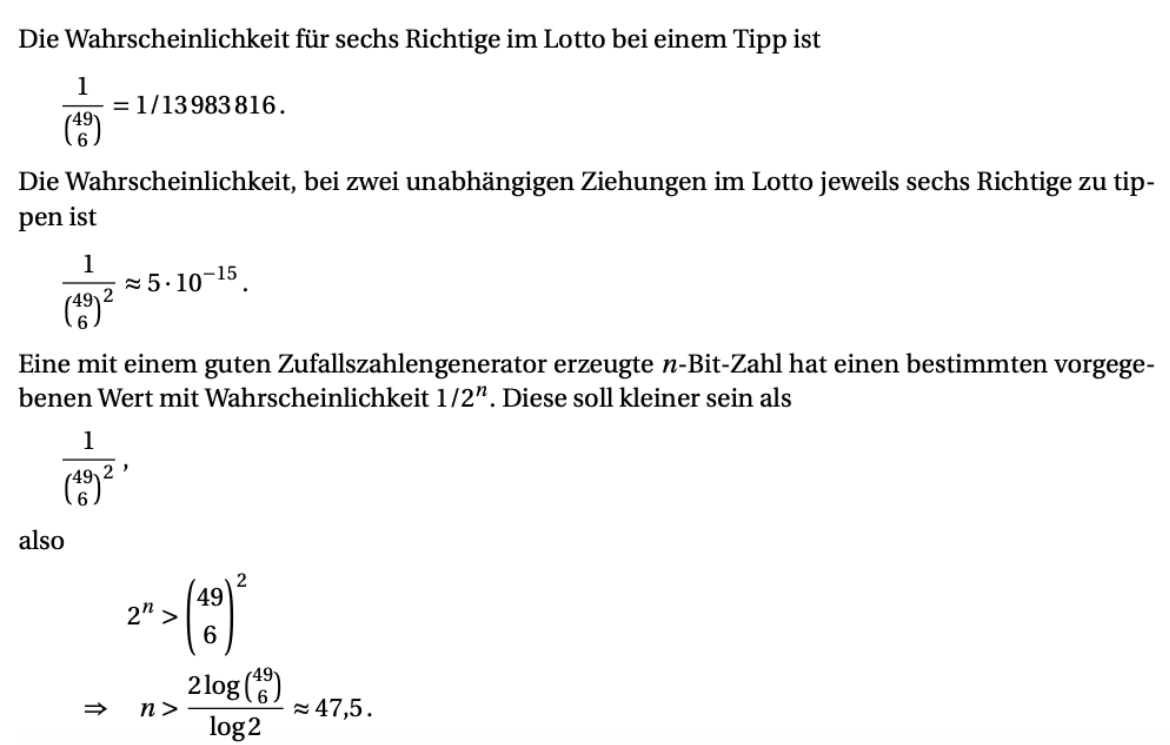
\includegraphics{img/bitcsol.png}

\newpage

    \hypertarget{aufgabe-5-secret-splitting}{%
\subsection{Aufgabe 5: Secret
Splitting}\label{aufgabe-5-secret-splitting}}

Sei Alices Identitätsinformation UID = 1000. Ist die folgende Gleichung
korrekt?

\[1000 = 9008 \oplus 8408\]

\hypertarget{solution}{%
\subsubsection{Solution}\label{solution}}

Zahlen in Binärsystem umwandeln und XORen:

8192 4096 2048 1024 512 256 128 64 32 16 8 4 2 1

9008 = 1 0 0 0 1 1 0 0 1 1 0 0 0 0\\
8408 = 1 0 0 0 0 0 1 1 0 1 1 0 0 0\\
XOR = 0 0 0 0 1 1 1 1 1 0 1 0 0 0 = 8 + 32 + 64 + 128 + 256 +512 = 1000

All good!

    

    \hypertarget{sw13---blockchain}{%
\section{SW13 - Blockchain}\label{sw13---blockchain}}

    \hypertarget{aufgabe-1-blockchain}{%
\subsection{Aufgabe 1: Blockchain}\label{aufgabe-1-blockchain}}

Erläutern Sie, inwiefern die dezentrale Architektur des
Blockchain-Netzwerkes zu dessen Sicherheit beiträgt.

\hypertarget{solution}{%
\subsubsection{Solution}\label{solution}}

Aufgrund der architektonischen Struktur bietet die Blockchain eine hohe
Sicherheit\\
und eine End-to-End-Transparenz. In einer Blockchain werden Daten anonym
gespeichert, dezentrale registriert und übermittelt. Diese Kombination
gewährleistet ein hohes Mass an\\
Sicherheit, „die auf sicherer Authentifizierung, Kennzeichnung und
Schutz der Daten basiert.

Eine Manipulation alter Transaktionen ist nicht einfach möglich, dafür
müssten alle Hashwerte der Folgeblöcke berechnet werden. Zusätzlich
müsste dann noch eine Mehrheit (51\%) der Nodes die ``neue'' Kette
akzeptieren.

    \hypertarget{aufgabe-2-elektronische-zahlungsverkehr}{%
\subsection{Aufgabe 2: Elektronische
Zahlungsverkehr}\label{aufgabe-2-elektronische-zahlungsverkehr}}

Woran unterscheidet sich E-Bargeld von Bitcoin? Nennen Sie mindestens 2
Punkte und begründen Sie Ihre Antwort.

\hypertarget{solution}{%
\subsubsection{Solution}\label{solution}}

\begin{enumerate}
\def\labelenumi{\arabic{enumi}.}
\item
  Unterschied: Trust

  \begin{itemize}
  \item
    E-Cash: Durch einen zentralen ``General Ledger'' (identisch mit
    traditionellem Geld).
  \item
    Blockchain als Basistechnologie für Bitcoin: Durch eine dezentrale
    Instanz namens ``Distributed Ledger''
  \end{itemize}
\item
  Unterschied: Eingesetzte Kryptographische Verfahren

  \begin{itemize}
  \item
    E-Cash: Braucht blinde Signatur (Chaum) einer zentralen Stelle
    (e.g.~Bank). Die zu\\
    übertragenden Einheiten werden mit einer Seriennummer versehen und
    im ``central ledger'' der 
    zentralen Instanz vermerkt. Asymmertrisches Verfaren zur Generierung
    von Schlüsseln basiert auf RSA.
  \item
    Bitcoin: Verwendet elliptische Kurven und asymmetrische
    Kryptographie (public key: walletadresse, 
    private key: signieren von Transaktionen).
  \end{itemize}
\end{enumerate}

    \hypertarget{aufgabe-3-bitcoin}{%
\subsection{Aufgabe 3: Bitcoin}\label{aufgabe-3-bitcoin}}

Nennen Sie die verwendeten kryptographischen Elemente für Bitcoin und
beschreiben Sie welche Funktionen sie erfüllen?

\begin{enumerate}
\def\labelenumi{\alph{enumi})}
\tightlist
\item
  Erläutern Sie, wie das Problem double-spending für Bitcoin gelöst
  wird?\\
\item
  Wie beurteilen Sie die ökologischen Aspekte in Bezug auf
  Energieverbrauch für Mining?\\
\item
  Was passiert im Jahre 2141, wenn kein Bitcoin mehr im Lauf gebracht
  wird?\\
\item
  Wie sicher ist Bitcoin gegen Cyberattacken? Kann Bitcoin verloren
  gehen?
\end{enumerate}

\hypertarget{solution}{%
\subsubsection{Solution}\label{solution}}

a.) Das Problem von double-spending wird durch die Arbeitsweise von den
Miners und\\
einen Cachespeicher (UTXO), der \textbf{Unspent Transaktionsoutputs} der
Blockchain gewährleiste.\\
Angenommen eine Absenderin Alice will eine Transaktion\\
durchführen. Der Miner überprüft erst die Verweise auf die
Inputstransaktionen\\
(Einzahlungen) von Alice: diese müssen mindestens den Betrag der
Outputstransaktionen\\
(Auszahlungen) abdecken. Dann überprüft der Miner über den UTXO, ob die
in der\\
Transaktion referenzierten Inputs noch nicht für andere Transaktionen
verwendet wurden\\
(wurde das Geld vorher schon ausgegeben-double-Spending?). Sollte das
der Fall sein wird\\
die Transaktion abgelehnt.

b.) Das Mining von Bitcoins verwendet eine sehr hohe Menge an Energie
für den POW, was ziemlich unökologisch ist.

c.) Im Jahr 2141 wird es keine neuen Bitcoins mehr geben für Mining
Aktivitäten, dann wird der maximale Betrag von 21'000'000 Bitcoins im
Umlauf sein.

d.) Die Blockchain von Bitcoin ist grundsätzlich Read-Only. Eine
Manipulation eines Blocks wird durch das verteilte System schnell
aufgedeckt (51\% Prinzip). Wenn jemand seinen Private-Key für sein
Wallet verliert, dann sind die Bitcoins darin auch verloren (gibt keine
Instanz die hier helfen könnte).

\newpage    

    \hypertarget{sw14---quanten-kryptografie}{%
\section{SW14 - Quanten
Kryptografie}\label{sw14---quanten-kryptografie}}

    \hypertarget{aufgabe-2-bb84}{%
\subsection{Aufgabe 2: BB84}\label{aufgabe-2-bb84}}

Suppose Alice uses the following polarization states and bit values and
Bob measures in the depicted basis. Compute the raw key (bevor
reconciliation/error correction and privacy amplification).

\begin{center}
	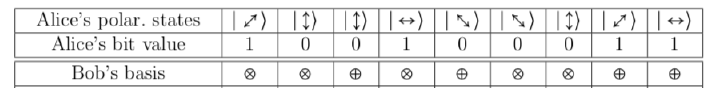
\includegraphics[scale=0.9]{img/ex02.png}
\end{center}

\hypertarget{solution}{%
\subsubsection{Solution}\label{solution}}

\begin{center}
	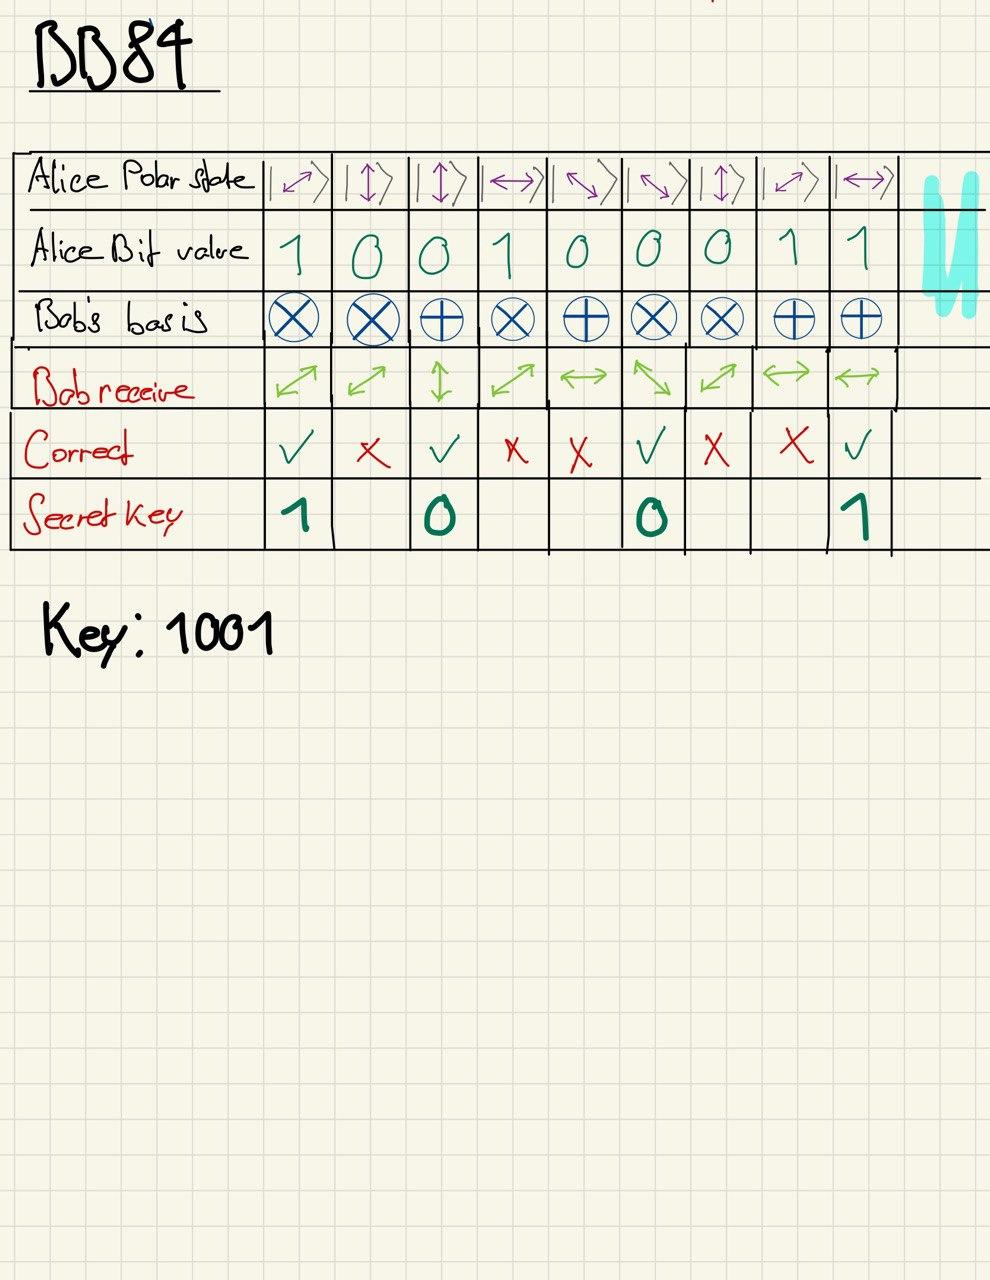
\includegraphics[scale=0.8]{img/bb84_1.jpg}
\end{center}

Gehen wir davon aus das "Eve" noch mithört muss noch ein 25\% Fehler eingebaut werden weil: \\
50\% W'Keit dass Basis H oder V ist multipliziert mit 50\% W'Keit das Eve die richtige Basis misst und an Bob weitersendet.

\newpage

    \hypertarget{aufgabe-3-again-bb84}{%
\subsection{Aufgabe 3: Again BB84}\label{aufgabe-3-again-bb84}}

In the BB84 protocol:

\begin{enumerate}
\def\labelenumi{\arabic{enumi}.}
\item
  what is the probability, that Bob chooses the same basis as Alice?

\begin{verbatim}
 50% (since he only has to choose horizontal or vertical)
\end{verbatim}
\item
  what is the probability, that Eve guesses the correct basis and
  resends the qubit in the correct state to Bob? Will her interaction be
  observed in this case?

\begin{verbatim}
 Eve has a 50% percent Chance to guess the correct basis.
 Eve has another 50% chance to resend the qubit in the
 correct state. So Eve produces an additional 25% Error Overall

 Bob/Alice could detect the listening, because Eve "destroys" the original Qubit with every listening and
 only has a 75% chance to restore it correctly.

 The Probability of Detection is: p = 1 - 0.75^n where n is number of qubits.
\end{verbatim}
\item
  What percentage of bits of the raw key has Bob to discard typically?
  Note: the shorter key is called shifted key.

\begin{verbatim}
 Also 50%
\end{verbatim}
\end{enumerate}

    \hypertarget{aufgabe-4-how-to-find-the-period-of-an-injective-function-f}{%
\subsection{Aufgabe 4: How to find the period of an injective function
f}\label{aufgabe-4-how-to-find-the-period-of-an-injective-function-f}}

The idea in classical computing would be to choose random \(x\) and
\(x'\) and check, whether \(f (x) = f (x')\).\\
If that is the case, then \(x' = x+kp\) for some \(k \in \mathbb{Z}\).
Hence we could find a multiple (\(kp\)) of the period \(p\).\\
It can be shown, that a first guess of \(p\) can be made using brute
force, by finding a collision in \(f\) using approximately \(\sqrt(r)\)
inputs. Explain!

\hypertarget{solution}{%
\subsubsection{Solution}\label{solution}}

Das Theorem ist Teil von Shors Algorithmus ``find period of a function
f''.

Es geht also darum zu schauen, ab wann sich eine Funktion wiederholt.
Als Beispiel nehmen wir \(2^{k} \mod 15\)

\(2^{0} \mod 15 = 1\)\\
\(2^{1} \mod 15 = 2\)\\
\(2^{2} \mod 15 = 4\)\\
\(2^{3} \mod 15 = 8\)\\
\(2^{4} \mod 15 = 1\)\\
\(2^{5} \mod 15 = 2\)\\
\(2^{6} \mod 15 = 4\)\\
\(2^{7} \mod 15 = 8\)

Man sieht schnell, das die Funktion sich nach 4 Schritten wiederholt.
somit ist \(p=4\) und es gilt \(2^{k} = 2^{k+p}\)

Anscheinend kann man hier das Geburtstags-Paradoxon anwenden und kommt
so auf \(\sqrt(r)\) inputs die man testen muss.

    \hypertarget{aufgabe-5-shors-algorithm-to-factor-35}{%
\subsection{Aufgabe 5: Shor's algorithm to factor
35}\label{aufgabe-5-shors-algorithm-to-factor-35}}

Use Shor's algorithm to factor \(n\) = 35. Start with \(m\) = 11, and
then \(m\) = 2, \(m\) = 3.\\
For step 2 use a classical computer, i.e.~do it by hand!

\hypertarget{solution}{%
\subsubsection{Solution}\label{solution}}

\begin{center}
	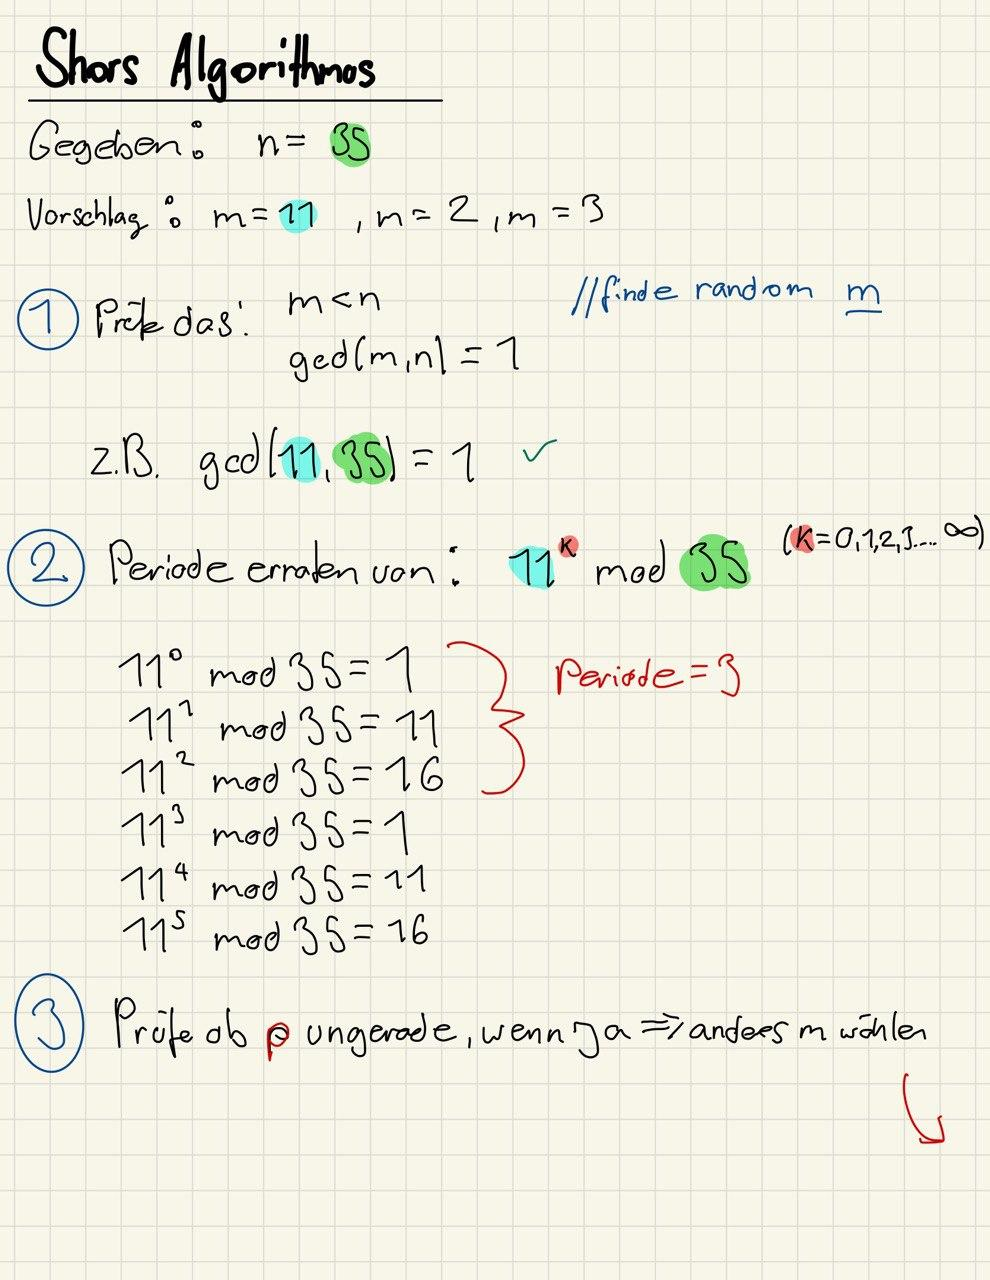
\includegraphics[scale=0.91]{img/shor1.jpg}\\
\end{center}

\break

\begin{center}
	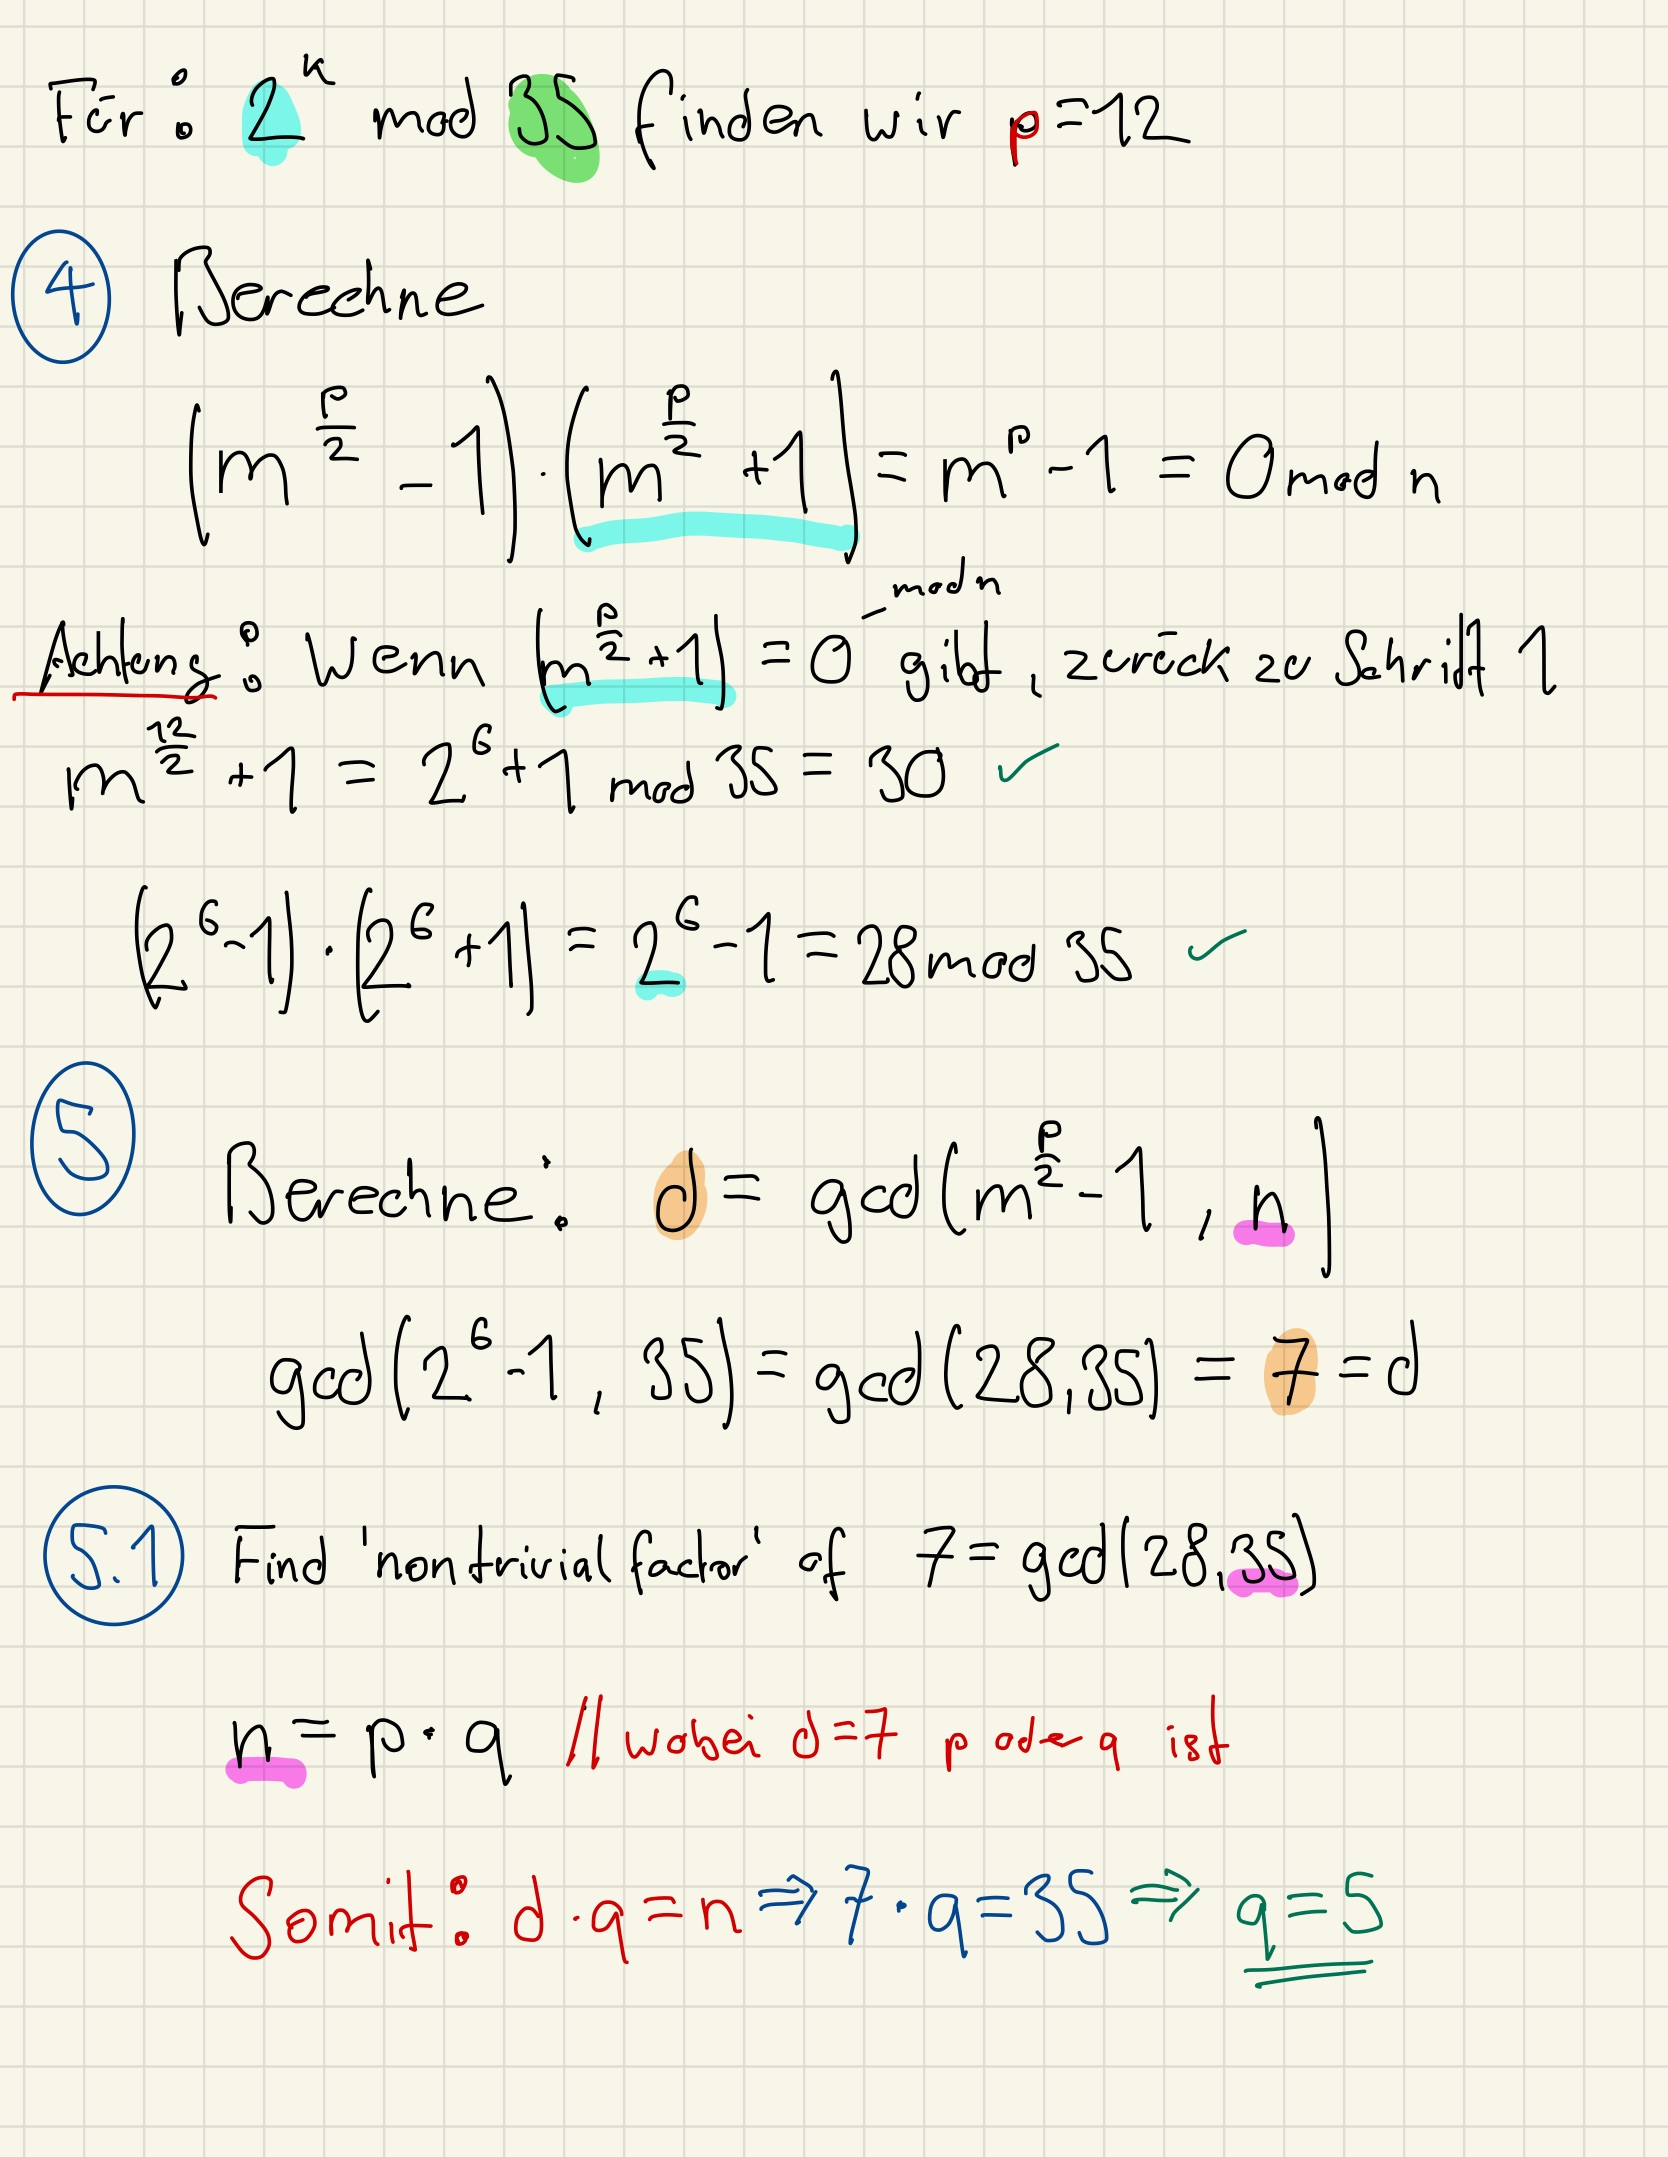
\includegraphics[scale=0.97]{img/shor2.jpg}\\
\end{center}



    % Add a bibliography block to the postdoc
    
    
    
\end{document}
